% !TeX document-id = {6b75a545-b662-4873-8f28-b81d849ea348}
% !TeX TXS-program:compile = txs:///latexmk/{}[-pdfxe -synctex=1 -interaction=nonstopmode -silent %]

\def\faqTitle{\LaTeX{} 常见问题}
\def\faqAuthor{\LaTeX{} Studio 团队}
\def\faqVersion{v0.5}

\documentclass{latex-faq-cn-class}

% 如果遇到字体问题,可以选择不使用自定义字体:
% \documentclass[use-customized-fonts=false]{latex-faq-cn-class}

% TODO: 移植到 class
% \makeatletter
% \def\@captype{figure}
% \makeatother

% % example-style1使用了lshort中示例样式
% %\usepackage{example-style1}
% % example-style2使用了mathfaq中示例样式
% \usepackage{example-style2}
% % mathfaq-style使用了mathfaq中一些设置
% \usepackage{mathfaq-style}
% % math-1包含了math部分需要在导言区设置的内容
% \DeclareMathOperator*{\esssup}{ess\,sup}

\usepackage{ifthen}
\newcounter{qlst}
\newenvironment{EqDesc}[2][式中]{%
	\begin{list}{}
		{%
			\usecounter{qlst}
			\settowidth{\labelwidth}{#1,\ \ #2\ --- \ }
			\setlength{\labelsep}{0pt}
			\setlength{\leftmargin}{\labelwidth}
			\setlength{\rightmargin}{0em}
			\setlength{\parsep}{0ex}
			\setlength{\itemsep}{0ex}
			\setlength{\itemindent}{0em}
			\setlength{\listparindent}{0em}
			\renewcommand{\makelabel}[1]
			{\stepcounter{qlst}
				\ifthenelse{\value{qlst}>1}{\hfill ##1\ --- \ }{#1,\hfill ##1\ --- \ }
			}
		}%
	}%
	{\end{list}}

\makeatletter
\def\ExtendSymbol#1#2#3#4#5{\ext@arrow 0099{\arrowfill@#1#2#3}{#4}{#5}}
\def\RightExtendSymbol#1#2#3#4#5{\ext@arrow 0359{\arrowfill@#1#2#3}{#4}{#5}}
\def\LeftExtendSymbol#1#2#3#4#5{\ext@arrow 6095{\arrowfill@#1#2#3}{#4}{#5}}
\makeatother

\newcommand\myRightarrow[2][]{\RightExtendSymbol{|}{=}{\Rightarrow}{#1}{#2}}
\newcommand\myArrow[2][]{\ExtendSymbol{\Leftarrow}{=}{\Rightarrow}{#1}{#2}}

\newenvironment{shrinkeq}[1]
{ \bgroup
	\addtolength\abovedisplayshortskip{#1}
	\addtolength\abovedisplayskip{#1}
	\addtolength\belowdisplayshortskip{#1}
	\addtolength\belowdisplayskip{#1}}
{\egroup\ignorespacesafterend}

\newcommand{\abs}[1]{\vert #1 \vert}

\begin{document}

% \tableofcontents

% \def\FONTTEST{字体测试骨头 ABC fi fl\ }
% \FONTTEST \textit{\FONTTEST} \textbf{\FONTTEST \textit{\FONTTEST}}          \par
% \textsf{\FONTTEST \textit{\FONTTEST} \textbf{\FONTTEST \textit{\FONTTEST}}} \par
% \texttt{\FONTTEST \textit{\FONTTEST} \textbf{\FONTTEST \textit{\FONTTEST}}}

\section*{前言}
本手册致力于打造最全面的中文 \LaTeX{}-faq。
在此感谢全体贡献手册内容的朋友。
建议使用
\begin{shcode}
  latexmk -pdfxe -synctex=1 -shell-escape latex-faq-cn
\end{shcode}
编译本文档。

如果您也是致力于发展中文 \LaTeX{} 的爱好者,请加入 \href{https://github.com/latexstudio/LaTeXFAQ-cn}{LaTeXFAQ-cn}
\clearpage
% Copyright (C) 2018 by latexstudio <http://www.latexstudio.net>
%
% This program is free software: you can redistribute it and/or modify
% it under the terms of the GNU General Public License as published by
% the Free Software Foundation, either version 3 of the License, or
% (at your option) any later version.
%
% This program is distributed in the hope that it will be useful,
% but WITHOUT ANY WARRANTY; without even the implied warranty of
% MERCHANTABILITY or FITNESS FOR A PARTICULAR PURPOSE.  See the
% GNU General Public License for more details.
%
% You should have received a copy of the GNU General Public License
% along with this program.  If not, see <http://www.gnu.org/licenses/>.
%

% !TEX root = ../latex-faq-cn.tex
% !TEX program = xelatex
% !TEX options = --shell-escape

\section{背景知识与基本概念}
\label{sec:basic}

\faq{什么是 \TeX{}?}{what-is-tex}

\TeX{} 是由著名计算机科学家 Donald~E. Knuth(高德纳)发明的排版系统。他在 \book{The \TeX book} 一书
的前言中曾提到:“(\TeX{})旨在创造美丽的书籍,尤其是那些包含很多数学公式的书。”
\footnote{原文如下:“This is a handbook about \TeX{}, a new typesetting system intended for the
creation of beautiful books---and especially for books that contain a lot of mathematics.”}

1976 年,Knuth 出版鸿篇巨著《计算机程序设计艺术》(\book{The Art of Computer Programming})第二卷
的第二版,但当时所用的照排技术却令他非常失望。作为斯坦福大学计算机科学系的教授,Knuth 决定自己开发
一套高质量的排版系统。1978年,他开发出了 \TeX{} 的第一个版本;随后,又在 1982 年推出了 \TeX{} 的
第二个版本(\TeX 82),也就是人们今天所用 \TeX{} 的基础。Knuth 将 \TeX{} 的源代码无偿发布在公有领域
\footnote{\TeX{} 使用的许可证为 \href{https://www.ctan.org/license/knuth}{Knuth License}。},
这使得他人可以进一步完善这一系统,并增加新的功能。

在今天,\TeX{} 既可以指 Knuth 发明的这一套排版系统,也可以指相应的排版语言,有时候也指将其打包、
整理以方便用户使用的软件套装(发行版)。

\begin{reference}
  \item https://texfaq.org/FAQ-whatTeX
  \item \TeX{}, Wikipedia, The Free Encyclopedia, \url{https://en.wikipedia.org/wiki/TeX}
\end{reference}


\faq{什么是 \LaTeX{}?}{what-is-latex}

\LaTeX{} 是 Leslie Lamport 在 \TeX{} 基础上创建的“文档准备系统”。Knuth 的 \TeX{} 虽然可以实现优美的
排版效果,但作者不得不挣扎在琐碎的排版细节之中。而 \LaTeX{} 则通过文档标记的手段,把很多格式细节
隐藏了起来,使得文档作者可以专注于内容本身,因此很快在学术界流行开来。

由此,我们可以看到,\LaTeX{} 最重要的一个原则,就是\strong{内容与格式分离}。文章作者只需要使用
\cs{title}、\cs{author}、\cs{section} 等命令以及 \env{proof}、\env{table} 这样的环境,而不需要操心
什么时候应该加粗、什么时候应该用斜体之类的排版细节。

然而,现实情况往往麻烦许多。\LaTeX{} 本身提供的功能还不够多,往往需要引入其他宏包来辅助排版;
另一方面,公式、图表一类的复杂元素远远不是若干文档标记就可以实现,高质量的排版仍离不开作者对各种
细节的精益求精。总之,如何在合适的层次做出取舍与平衡,正是 \LaTeX{} 进一步发展所需要考虑的。

\begin{reference}
  \item Introduction to \LaTeX{}, \url{https://www.latex-project.org/about}
  \item https://texfaq.org/FAQ-latex
  \item \LaTeX{}, Wikipedia, The Free Encyclopedia, \url{https://en.wikipedia.org/wiki/LaTeX}
\end{reference}


\faq{\TeX{} 中常见术语的解释}{tex-terms}

\begin{description}
  % TODO
%  \item[引擎] \LaTeX{}/\TeX{} 解析引擎,其实就是一个编译器,它输入一个 |.tex| 文件作为输入,根据
%    源文件的内容送入解析引擎和渲染引擎进行处理,并将排版的成果——文档编译输出,\LaTeX{}/\TeX{} 的
%    解析引擎目前有pdflatex、xelatex、lualatex等,它们都可以输出pdf文档文件(部分解析器可以输出dvi
%    文件),用于在多平台进行分发甚至打印出版。
  \item[引擎] \LaTeX{}/\TeX{} 解析引擎,其实就是一个编译器,它输入一个 |.tex| 文件作为输入,根据
  源文件的内容送入解析引擎和渲染引擎进行处理,并将排版的成果——文档编译输出,\LaTeX{}/\TeX{} 的解
  析引擎目前有\pdfTeX{}、\XeLaTeX{}等。
  \item[格式] \TeX{} 是存在各种不同的封装格式的,比如原生的 \TeX{} 或者 \LaTeX{},我们所使用的
    \LaTeX{} 只是\TeX{} 封装格式的其中一种,是目前流行的封装规范。
  \item[发行版] \LaTeX/\TeX{}都包含了成千上万个宏包,甚至有可能我们需要安装新的宏包,除了手动安装
    外,最好的方式就是利用发行版的宏包管理器,所谓发行版就是把\LaTeX/\TeX{}的相关组件打包,形成一个
    独立完善的\LaTeX/\TeX{}系统,目前流行的发行版有MiKTeX、proTeXt 以及TeXLive。
  \item[编译命令] 是实际调用的、结合了引擎和格式的命令。如 |xelatex| 命令是结合\XeTeX{}引擎和
  \LaTeX{}格式的一个编译命令。
\end{description}


% \faq{不同的TeX封装格式的区别?}[tex-format]
% TODO: 该问题跟上下两个重复
%
% \textbf{原生\TeX{}}
%
% TeX本身是一个基于控制序列的排版系统,它指示TeX如何在页面上放置文本。例如,|\hskip|指在文档中在
% 文档中插入一定数量的水平空间,而|\font|是指给文档中的文字定义一种给定的字体。TeX是完全可编程的,
% 它使用一种集成的宏脚本语言,支持变量,范围,条件执行,控制流和函数定义等。
%
% \textbf{TeX宏包(\TeX{}格式)}
%
% TeX的一些控制序列直接使用是单调乏味的;它们主要作为更高层次的构建快,因此更易于用户使用。例如,
% 在基础TeX中没有办法能够制定一段文字应该排版为更大的字体,相反,你必须了解当前的字体和大小,然后
% 加载一种同样字体但更大字号的字体。幸运的是,TeX是可编程的,它可以通过写一个宏将这些复杂性都隐藏在
% 一个简单的,新的控制序列之后。例如,我们可以通过 |\larger{my text}| 将“my text”定义为比当前更大的
% 字体。一些使用者会写一些完全由自己定义的宏集,然后再一些文档中重复使用,但,常见的还是依赖于由专家
% 编写的TeX宏包——一些宏的集合。为了方便用户,这些宏包通常与基本的TeX引擎结合到一个独立的可执行的
% 文件中。
%
% \textbf{TeXLive、MacTeX、MikTeX、CTex}
%
% TeXLive 由类 UNIX 系统上的 teTeX 发展并取而代之,最终成为跨平台的 TeX 发行版。TeXLive 自 2011 年
% 起以年份作为发行版的版本号,保持了一年一更的频率。MacTeX 是 macOS(OS X)系统下的一个定制化的
% TeXLive 版本,与 TeXLive 同步更新。MikTeX 是主要用于 Windows 平台的一个稳定发展的 TeX 发行版,
% 目前已开发出跨平台版本。中国的 LaTeX 用户应该对“CTeX 套装”比较熟悉,它是一个经过本地化配置的
% MikTeX,目前已不推荐使用。


\faq{\TeX{} 有哪些格式?}{tex-format}

\TeX{} 是一种排版文件的计算机程序,它需要一个计算机文件,根据 \TeX{} 的规则进行准备,并将其转换成
一种可以在高质量打印机上打印的形式,比如激光打印机,可以打印出一份与高质量的书籍和期刊相媲美的打印
文档。不包含数学公式或表格的简单文档可以很容易就生成,事实上,所有人都必须直接输入文本(只是遵循
不同的符号规则)。输入数学公式时比较复杂的,但当考虑到产生一些数学公式的复杂性时,\TeX{} 是相对容易
使用的,它可以产生大量的数学符号。

\TeX{} 包括各种不同的“方言”,其中包括 \LaTeX{}。\PlainTeX{} 是 \TeX{} 中最基础的版本,也是其他
“方言”的基础。为了用 \TeX{} 生成文档,我们必须首先在计算机上创建一个合适的输入文件,我们将 \TeX{}
程序应用到输入文件中,然后再用打印机打印由 \TeX{} 程序生成的所谓的“DVI”文件。

\begin{description}
  \item[\PlainTeX] Knuth 设计了一个名叫 \PlainTeX{} 的基本格式,以与低层次的原始 \TeX{} 呼应。
    这种格式是用 \TeX{} 处理文本时相当基本的部分,以致于我们有时都分不清到底哪条指令是真正的处理
    程序 \TeX{} 的原始命令,哪条是 \PlainTeX{} 格式的。大多数声称只使用 \TeX{} 的人,实际上指的是
    只用 \PlainTeX{}。

    \PlainTeX{} 也是其它格式的基础,这进一步加深了很多人认为 \TeX{} 和 \PlainTeX{} 是同一事物的
    印象。\PlainTeX{} 的重点还只是在于如何排版的层次上,而不是从一位作者的观点出发。对它的深层功能
    的进一步发掘,需要相当丰富的编程技巧。因此它的应用就局限于高级排版和程序设计人员。

    有关 \PlainTeX{} 的相关信息可见:\url{http://www.ntg.nl/doc/wilkins/pllong.pdf}

  \item[\LaTeX] 有两个版本,分别是 \LaTeXe{} 和 \LaTeX2.09,前者是当前使用的版本,后者是在 1994 年
    首次发布的公开版本,但现已过时。因此,\LaTeX{} 与 \LaTeXe{} 实际上是同义词。

    Leslie Lamport 开发的 \LaTeX{} 是当今世界上最流行和使用最为广泛的 \TeX{} 格式。它构筑在 Plain
    \TeX{} 的基础之上,并加进了很多的功能以使得使用者可以更为方便的利用 \TeX{} 的强大功能。使用
    \LaTeX{} 基本上不需要使用者自己设计命令和宏等,因为它已经替你做好了。因此,即使使用者并不是很
    了解 \TeX{},也可以在短时间内生成高质量的文档。对于生成复杂的数学公式,\LaTeX{} 也表现得更为
    出色。

    \LaTeX{} 自从二十世纪八十年代初问世以来,也在不断的发展。最初的正式版本为 2.09,在经过几年的
    发展之后,许多新的功能,机制被引入到 \LaTeX{} 中。在享受这些新功能带来的便利的同时,它所伴随的
    副作用也开始显现,这就是不兼容性。标准的 \LaTeX2.09,引入了“新字体选择框架”(NFSS)的 \LaTeX{}、
    % TODO
    SLiTeX、AMSLaTeX 等等,相互之间并不兼容。这给使用者和维护者都带来很大的麻烦。

    为结束这种糟糕的状况,Frank Mittelbach 等人成立了 \LaTeX3 项目小组,目标是建立一个最优的、有效
    的、统一的、标准的命令集合,即得到 \LaTeX{} 的一个新版本 3。这是一个长期目标,向这个目标迈出
    第一步就是在 1994 年发布的 \LaTeXe{}。\LaTeXe{} 采用了 NFSS 作为标准,加入了很多新的功能,同时
    还兼容旧的 \LaTeX2.09。\LaTeXe{} 每 6 个月更新一次,修正发现的错误并加入一些新的功能。在
    \LaTeX3 最终完成之前,\LaTeXe{} 将是标准的 \LaTeX{} 版本。

  \item[\ConTeXt] \ConTeXt{} 是 \TeX{} 的一种格式,是 Hans Hagen 和荷兰 Pragma-ADE 公司设计的一种
    高端的文档制造工具,官方网站为 \href{http://wiki.contextgarden.net}{\ConTeXt{} Garden}。
    \ConTeXt{} 就像 \LaTeX{} 是基于 \TeX{} 排班系统的文档制作系统,如果说 \LaTeX{} 将作者从排版的
    细节中隔离出来,那么 \ConTeXt{} 就是采用一种互补的方法来处理结构化的界面来处理排版,包括对
    颜色、背景、超链接、演示文稿、图形文本集成和条件编译的广泛支持, 对于数学、化学等科技文档的支持
    同等优秀甚至更为方便,而且其为了更容易实现各种华丽排版效果。它可以让用户对格式进行广泛的控制,
    同时又可以在不需要学习 \TeX{} 宏语言的情况下轻松地创建新的布局和样式。 因此 \ConTeXt{} 的图形
    功能要远远强于 \TeX{} 和 \LaTeX{},可以制作非常漂亮的 PDF 文档,特别适合做幻灯片和一些非正式的
    文档。

    \ConTeXt{} 将 \METAFONT{}、\METAPOST{} 的超集以及一个强大的矢量图形系统整合起来。\MetaFun{}
    可以作为一个独立的系统来生成数据,但是它的优势在于用精确的图形元素来增强 \ConTeXt{} 文档。

    目前,\ConTeXt{} 主要分为两个版本,分别是 Mark II 和 Mark IV(MkII 和 MkIV)。前者已处于稳定
    状态,只进行代码维护;而后者仍在活跃开发中。MkII 默认使用 \pdfTeX{} 引擎;而 MkIV 由于采用了
    新的字体机制,仅支持 \LuaTeX{} 引擎。(\LuaTeX{} 的发展也是由于 \ConTeXt{} 驱动)。

    注:CTAN 不支持 \ConTeXt{} 的发布。潜在的用户可以去
    \href{http://wiki.contextgarden.net/Main_Page}{ConTeXt Garden} 了解当前发行版的详细信息。

  \item[Texinfo] TeXinfo 是一个使用同一个源文件生成在线信息和打印输出的文档系统,所以只需要编写一个
    文档源文件,当工作被修改时,只需要修改源文件即可。其源文件的后缀名为 |texi| 或 |texinfo|。

    TeXinfo 是一门宏语言,就像 \LaTeX{} 一样,但是它的表达能力略弱,它的表观与 \TeX{} 的其他宏语言
    相似,只不过它的宏要以 |@| 开头,而 \TeX{} 系统中用 |\| 开头。

    你可以在 GNU Emacs 中编写以及将 TeXinfo 文件转化成 info 文件,你也可以在 makeinfo 中将 TeXinfo
    文件转换成 info 文件,然后再 info 中阅读,所以也不是必须依赖于 Emacs。这个发行版包括一个 Perl
    脚本,|texi2html|,可以将 TeXinfo 文件转换成 HTML,这种语言比 \LaTeX{} 更适合 HTML,所以将
    \LaTeX{} 转换成 HTML 的痛苦就可以避免了。

    当然,你也可以用 \pdfTeX{} 将输入文件转换成 PDF 格式。makeinfo 可将 texinfo 文档转换成 HTML、
    DocBook、Emacs info、XML 和纯文本。\TeX{}(或者 |texi2dvi| 和 |texi2pdf|),因为 \TeX{} 加载了
    普通的 \TeX{} 宏,而并不是 TeXinfo,所以 TeXinfo 文档必须以 \verb|\input texinfo \verb| 开头来加载
    \pkg{texinfo} 包。

  % TODO: 不常用,可删去
  \item[Eplain] Eplain 扩展并延伸了 \PlainTeX{} 的定义,它并不像 \ConTeXt{}。
\end{description}


\faq{\LaTeX2.09 和 \LaTeXe{} 有什么区别?}{latex2.09-latex2e-diff}

后者是前者的改进。从文件内容上看,两者最显著的不同在于 \LaTeX2.09 使用 |\documentstyle| 命令定义
文档类以及所包含宏包,如:

\begin{texinlist}
\documentstyle[twoside,epsfig]{article}
\end{texinlist}

而 \LaTeX2e{} 使用 |\documentclass| 命令设置文档类型,用 |\usepackage| 命令调用宏包。


\faq{\TeX{}, \LaTeX{}, pdflatex, xelatex, xetex等的区别和关系,什么时候用什么编译器编译}
  {build-all-diff}
% TODO: 非常混乱……

LaTeX 其实是目前使用最广泛的 \TeX{} 格式。xeTeX 是一种引擎(编译器),pdfLaTeX (xeLaTeX) 是命令,
他们分别结合了 pdfTeX(xeTeX) 引擎和 \LaTeX{} 格式。对于刚开始接触的人,建议处理英文时直接使用
pdfLaTeX,处理非英文时使用 XeLaTeX(并且用utf-8编码源文件)


%\faq{文本文件编码解读}{encoding}


\faq{\LaTeX{} 的源文件有什么要求?}{latex-source-file}

\LaTeX{} 的源文件是 |*.tex| 文件,是指 latex 编译器处理输入文件的源码,latex 编译器会对输入文件进行
解析,构造解析树,进行渲染,然后输出处理后的文档,完成一次编译过程,由于 \LaTeX{} 解析器可能对中文
文件名处理存在兼容性问题,不建议将 \LaTeX{} 的源文件的文件名设置为中文。


\faq{连字符如何在 \TeX{} 起作用?}{hyphen}
% TODO: 不应该放在这里,给的例子也很奇怪

如果 \LaTeX{} 遇到了很长的英文单词,仅在单词之间的位置断行无法生成宽度匀称的行时,就要考虑从单词
中间断开。对于绝大部分单词,\LaTeX{} 能够找到合适的断词位置,在断开的行尾加上连字符 |-|。如果一些
单词没能自动断词,我们可以在单词内手动使用 |\-| 命令指定断词的位置,如:

\begin{texinlist}
I think this is: su\-per\-cal\-%
i\-frag\-i\-lis\-tic\-ex\-pi\-%
al\-i\-do\-cious.
\end{texinlist}


%\faq{Unicode 和 \TeX{}}{unicode-and-tex}


\faq{常见的 \TeX{} 文件扩展名与文件用途}{extensions}
% TODO: 见如下链接
%   https://tex.stackexchange.com/q/7770/136923
%   https://tex.stackexchange.com/q/53240/136923
%   https://github.com/wspr/latex-auxfiles

常见的用户文件的扩展名与其用户如下:
\begin{itemize}
  \item |.tex| 文件。源文件,需用户编写。
  \item |.sty| 宏包文件。宏包的名称就是去掉扩展名的文件名。
  \item |.cls| 文档类文件。同样地,文档类名称就是文件名
  \item |.bib| \BibTeX{} 参考文献数据库文件。
  \item |.bst| \BibTeX{} 用到的参考文献格式模板。
  \item |.log| 排版引擎生成的日志文件,供排查错误使用。
  \item |.aux| \LaTeX{} 生成的主辅助文件,记录交叉引用、目录、参考文献的引用等。
  \item |.toc| \LaTeX{} 生成的目录记录文件。
  \item |.lof| \LaTeX{} 生成的图片目录记录文件。
  \item |.lot| \LaTeX{} 生成的表格目录记录文件。
  \item |.bbl| \BibTeX{} 生成的参考文献记录文件。
  \item |.blg| \BibTeX{} 生成的日志文件。
  \item |.idx| \LaTeX{} 生成的供 \pkg{makeindex} 处理的索引记录文件。
  \item |.ind| \pkg{makeindex} 处理 |.idx| 生成的格式化索引记录文件。
  \item |.ilg| \pkg{makeindex} 生成的日志文件。
  \item |.out| \pkg{hyperref} 宏包生成的 PDF 书签记录文件。
\end{itemize}


\faq{什么是 DVI 文件?}{what-is-dvi}
% TODO: 部分内容重复

DVI(device independent)文件为 \TeX{} 电子排版系统的输出文件。七十年代末,Knuth 在看到其多卷巨著
《The Art of ComputerProgramming》第二卷的校样时,对由计算机排版的校样的低质量感到无法忍受。因此
决定自己来开发一个高质量的计算机排版系统,这样就有了 TeX。TeX 的输出文件称为 DVI 文件,即是“Device
Independent”。一旦 TeX 处理了你的文件,你所得到的 DVI 文件就可以被送到任何输出设备,如打印机、屏幕
等并且总会得到相同的结果,而这与这些输出设备的限制没有任何关系。这说明 DVI 文件中所有的元素,
从页面设置到文本中字符的位置都被固定,不能更改。


\faq{什么是 TDS?}{what-its-tds}

TDS 全称 \TeX{} Directory Structure,意为 \TeX{} 目录结构,即 \TeX{} 发行版的文件组织结构。大部分
\TeX{} 发行版都将自身的文件组织成相近的路径结构,也就是 TDS。TDS 也称为 TEXMF 树,这是 \TeX{} 与
\METAFONT{} 的合称。很多系统的 TDS 结构都以 |texmf| 或者类似的词作为 TEXMF 树的根目录名,如在
\TeXLive{} 中,安装目录下的 |texmf-dist|、|texmf-var| 等就是两个不同的 TEXMF 树,
如图~\ref{fig:texmf-dir}。

\begingroup
  \dirtree {%
    .1 TEXMF树.
    .2 bibtex/\DTcomment{\BibTeX{} 相关文件}.
    .3 bib/\DTcomment{公用 bib 数据库}. % TODO: verb 有问题
    .3 bst/\DTcomment{格式文件}.
    .2 doc/\DTcomment{各类用户文档}.
    .3 bibtex/\DTcomment{\BibTeX{} 相关文档}.
    .3 fonts/\DTcomment{字体文档}.
    .3 generic/\DTcomment{通用于各种格式的文档}.
    .4 pgf/.
    .5 pgfmanual.pdf\DTcomment{PGF/\TikZ{} 用户手册}.
    .3 latex/\DTcomment{用于 \LaTeX{} 格式的文档}.
    .4 ctex/.
    .5 ctex.pdf\DTcomment{\CTeX{} 宏集用户手册}.
    .5 README.md\DTcomment{\CTeX{} 宏集简短介绍}.
    .3 texlive/\DTcomment{\TeXLive{} 发行版自身的文档}.
    .2 font/\DTcomment{字体相关文件}.
    .3 opentype/\DTcomment{OpenType 格式的字体}.
    .3 source/\DTcomment{字体源代码}.
    .3 truetype/\DTcomment{TrueType 格式的字体}.
    .3 type1/\DTcomment{Type1 格式的字体}.
    .2 scripts/\DTcomment{可执行脚本}.
    .3 l3build/\DTcomment{\LaTeX{} 构建、测试脚本}.
    .3 latexmk/\DTcomment{自动编译系统}.
    .3 texdoc/\DTcomment{文档查询系统}.
    .2 source/\DTcomment{源代码}.
    .3 bibtex/\DTcomment{\BibTeX{} 相关宏包代码}.
    .3 fonts/\DTcomment{字体源代码}.
    .3 generic/\DTcomment{通用于各种格式的宏包代码}.
    .3 latex/\DTcomment{用于 \LaTeX{} 格式的宏包代码}.
    .4 ctex/\DTcomment{\CTeX{} 宏集源代码}.
    .5 ctex.dtx.
    .5 ctex.ins.
    .5 ctexpuct.spa.
    .2 tex/\DTcomment{\TeX{} 宏,可被引擎读入}.
    .3 generic/\DTcomment{通用于各种格式}.
    .3 latex/\DTcomment{用于 \LaTeX{} 格式}.
    .4 base/\DTcomment{\LaTeX{} 的基本宏文件}.
    .5 article.cls.
    .5 book.cls.
    .5 report.cls.
    .5 latex.ltx.
    .4 beamer/\DTcomment{\cls{beamer} 宏集相关文件}.
    .4 ctex/\DTcomment{\CTeX{} 宏集相关文件}.
    .5 ctexart.cls.
    .5 ctexbeamer.cls.
    .5 ctexbook.cls.
    .5 ctexrep.cls.
    .5 ctex.sty.
    .3 plain/\DTcomment{用于 \PlainTeX{} 格式}.
    .3 xetex/\DTcomment{用于 \XeTeX{} 引擎}.
    .3 xelatex/\DTcomment{用于 \XeTeX{} 引擎下的 \LaTeX{} 格式}.
    .4 xecjk/\DTcomment{\pkg{xeCJK} 宏包相关文件}.
    .5 xeCJK.sty.
  }
  \captionof{figure}{TEXMF 树目录结构}
  \label{fig:texmf-dir}
\endgroup
(来自刘海洋《LaTeX 入门》)

%\faq{从TeX编写(文本)文件}{tex-text-write}

%\faq{\\special命令}{special-command}

\faq{Overleaf 是什么?如何使用?}{overleaf}

\href{https://www.overleaf.com}{Overleaf} 是一个在线的 \LaTeX{} 协作平台,可在各大浏览器内运行,
也就是说,不需要本地安装 \LaTeX{} 套装,就可以撰写编译 \LaTeX{} 文件。2017 年 Overleaf 与另一家
在线 \LaTeX{} 平台 \href{https://www.sharelatex.com}{ShareLaTeX} 合并,新的
\href{https://v2.overleaf.com}{Overleaf v2 平台} 囊括了两个原先平台的主要功能,而原有的 Overleaf 和
ShareLaTeX 用户可以在 Overleaf v2 上继续编辑原先所有的项目文件。

由于个别地区、单位的网络问题或限制,有些用户可能无法顺利登录、访问 Overleaf,在此我们不作
(也不方便)讨论。

Overleaf v1 目前运行的是 \TeXLive{} 2016,Overleaf v2 则是 \TeXLive{} 2017。升级 \TeXLive{} 2018
可能需要等到 2019 年。Overleaf v1 和 v2 都支持 \LaTeX{} + dvipdf、\pdfLaTeX{}、\XeLaTeX{}、
\LuaLaTeX{} 等多种编译方式;通过 |latexmkrc| 设置也可用 \pTeX{} 等其它编译器。支持中文,可以用
传统手段 \pkg{CJK} 宏包
\footnote{示例见 \url{https://www.overleaf.com/read/xhzmbjjnbfrq}。},
也可用 \CTeX{} 宏集的新一代解决方案
\footnote{示例见 \url{https://www.overleaf.com/read/gndvpvsmjcqx}。},
当然我们比较推荐后者。由于字库版权问题,Overleaf 上不会有 Windows 中文字体可用,因此如果一定要用
Windows 中文字体的话(高校论文要求等原因),则还是建议本地编译。毕竟字库文件太大,逐个上传还是
比较麻烦。

Overleaf 用的服务器系统是 Ubuntu Linux,因此文件名区分大小写。编译时用的是 \pkg{latexmk},因此在
Overleaf上每“编译”一次,其实可能已经运行了 4 次 |xelatex| + 1 次 |bibtex| + 1 次 |makeglossaries|
等等,把所有交叉引用、文献引用等等都解决掉,也可以自动调用 |biber| 或 \pkg{biblatex},或自动编译
\pkg{chapterbib}、\pkg{multibib} 所导出的多个文献列表。

Overleaf 编译也自动启用 |--shell-escape|,因此 \pkg{minted}、\pkg{tikz-externalize} 
等都可以使用。|--shell-escape| 本来是有安全隐忧的,但是每个 Overleaf 文件项目都是一个单独的 Docker 
容器(container),因此若是有谁想玩什么把戏,也不会波及其它项目。

【其它重点功能介绍明天,不,有空时再补充:multi-authors collaboration, RichText mode,
Overleaf Gallery and templates, one-click submission to journals, git bridge and github sync,
history tracking, 文件项目空间上限】

如果对 Overleaf 有任何问题,建议直接发送电子邮件至
\href{mailto:support@overleaf.com}{support@overleaf.com} 询问,不必过多自行揣测。若是担心语言沟通
问题,大可放心——Overleaf 技术支援人员有熟悉中文的。

%\pkg{minted} 在 Overleaf v1、v2 都是可以用的,例子参照
%\url{https://www.overleaf.com/read/qphhfvnsddbs}。MATLAB 高亮也一样可以用 \pkg{minted} 完成,注意
%字母大小写:
%
%\begin{verbatim}
%\begin{minted}{matlab}
%...
%\end{minted}
%\end{verbatim}
%
%Overleaf v1 的确有文件数目及项目大小限制,视收费与否而定:\url{https://www.overleaf.com/help/297};
%Overleaf v2 则相对宽松得多:所有项目(包括免费)都无文件大小上限,条件:每个项目限 2000 文件,以及
%可编辑纯文本文件不大于 5MB。详见
%\url{https://www.sharelatex.com/learn/Uploading_a_project#Limitations_on_Uploads}。
%
%Overleaf v1 是支持两层及以上的文件夹的,详情看 \url{https://www.overleaf.com/help/187};
%Overleaf v2 可以直接右键资料夹,再创建子资料夹。
%
%Overleaf v2 目前还是比较稳定的(2018 年 9 月将会全面上线)。当然如果是特定地区、单位限制的原因,
%则不方便在这里讨论。
%
%【这里先预定个位置,以后可以写个篇幅比较长的功能介绍。若对 Overleaf 有任何问题,建议直接电邮
%support@overleaf.com 询问,不必过多自行揣测。若是担心语言问题,Overleaf 技术支援人员有谙中文的。】

\faq{编译器与编辑器的区别是什么?}{ide-compile-diff}

在 \pkg{lshort} 中,确切解释了,所谓编译器,真正的名称叫排版引擎,是读入源代码并编译生成文档的
程序,如 \pdfTeX{}、\XeTeX{} 等。

编辑器,其实是用户书写源代码的工具,例如 Windows 下的记事本、Ubuntu 下的 gedit 等等。目前很多编辑器
都提供了“编译”按钮,本质上是基于命令行调用了编译器。

\faq{未来有计划做到像 Bakoma 那样所见即所得吗?}{bakoma}

\LaTeX{} 的缺点之一,相比“所见即所得”的模式有一些不便,为了查看生成的文档,用户总要不停地编译。  

% \faq{什么是“决议”(resolutions)}
% \faq{什么是(\TeX{})宏}
% \faq{什么是\LaTeX{}类和工具包}
% \faq{什么是PK文件}
% \faq{什么是TFM文件}
% \faq{什么是编码}
% \faq{什么是EC字体}
% \faq{什么是虚拟字体}
% \faq{什么是“Encapsulated PostScript”(EPS)}
% \faq{什么是DVI驱动程序}
% \faq{什么是“Berry命名方案”}

% Copyright (C) 2018 by latexstudio <http://www.latexstudio.net>
%
% This program is free software: you can redistribute it and/or modify
% it under the terms of the GNU General Public License as published by
% the Free Software Foundation, either version 3 of the License, or
% (at your option) any later version.
%
% This program is distributed in the hope that it will be useful,
% but WITHOUT ANY WARRANTY; without even the implied warranty of
% MERCHANTABILITY or FITNESS FOR A PARTICULAR PURPOSE.  See the
% GNU General Public License for more details.
%
% You should have received a copy of the GNU General Public License
% along with this program.  If not, see <http://www.gnu.org/licenses/>.
%

\section{最常出现的问题}
\label{sec:starter}

\faq{论文 / 比赛的 deadline 要到了,如何在一天 / 两天 / 三天之内入门 \LaTeX{}?}%
  {get-started-in-a-short-time}

非常遗憾,这几乎是不可能完成的任务。在时间紧张、压力巨大的情形下,入门 \LaTeX{} 对您来说没有意义。
作为排版工具,\LaTeX{} 实现的效果远没有文章的内容重要,所以请不要在这种情况下把您的精力投入在学习
\LaTeX{} 上。

通常来说,我们建议您至少通过三个月的时间来入门 \LaTeX{},并在之后的工作、学习中不断深入理解、
积累经验。

如果确有必要在短时间内掌握 \LaTeX{} 的使用方法,请联系靠谱且有经验的人。注:很多“学长”、“老师”都是
不靠谱的,所以这一点实际上很难办到。


\faq{我是新手,学习 \LaTeX{} 应该怎么入门?}{get-started}

首先,您需要确保自己有较为充裕的时间。接下来,我们推荐您阅读一些 \LaTeX{} 入门材料,比较知名的有
\href{http://mirrors.ctan.org/info/lshort/chinese/lshort-zh-cn.pdf}{《一份不太简短的 \LaTeXe{} 介绍》}
(\href{http://mirrors.ctan.org/info/lshort/english/lshort.pdf}{\book{The Not So Short In­tro­duc­tion to \LaTeXe{}}}),
即 \pkg{lshort}。此外,您还需要在电脑上安装一套发行版(见\faqref{install-latex}),或使用在线服务,
如 \href{https://www.overleaf.com/}{Overleaf}、\href{https://www.sharelatex.com}{ShareLaTeX} 等。

进一步的学习还需要阅读更多的书籍和文档,例如刘海洋《\LaTeX{} 入门》
\footnote{如作者所言,“虽然书名是《入门》,不过其实我并非完全是按新手入门的节奏在写,除了第一章是
  零基础入门,后面的内容编排并不完全是从基础到深入的顺序,而是按主题划分;实际内容上也包含一些比较
  专门的东西”,这本书内容丰富、讲解深入,但对新手未必友好。而且需注意,关于中文处理的部分可能略显
  过时。}。
此外,善用搜索引擎
\footnote{对于技术方面的问题,我们不很推荐百度。谷歌在大多数时候都可以获得更好的搜索结果;当然,
  如果您身处国内,必应很可能是更好的选择。}
也是必备技能。最后,我们强烈建议您提高英语水平,因为 \LaTeX{} 的相关材料,除了中文排版相关,几乎
都是英文的。

\begin{reference}
  \item 刘海洋.自学 \LaTeX{} 可以读什么书入门?.
    \url{https://www.zhihu.com/question/26645810/answer/33515971}
  \item milksea.新手请先读我.\url{http://bbs.ctex.org/forum.php?mod=viewthread&tid=48244}
\end{reference}


\faq{如何“安装 \LaTeX{}”?}{install-latex}

如果您也有这一问题,首先需要澄清一些概念,见\faqref{tex-related-things}。简短来说,\LaTeX{} 本身是
一种标记语言,而不是 Microsoft Word 一样现成的软件。因此,社区将相关的支持文件、可执行程序、文档等
打包在了一起,形成了可供用户下载、安装的发行版(distribution)。一般而言,“安装 \LaTeX{}”指的就是
安装发行版。

目前,根据平台不同,可供使用的主流发行版有以下这些:

\begin{itemize}
  \item \TeXLive{},见\faqref{install-texlive}
  \item \MiKTeX{},见\faqref{install-miktex}
  \item \MacTeX{},适用于 macOS,见\faqref{install-mactex}
  \item pro\TeX{}t,见\faqref{download-protext}
  % TODO: 更多的发行版介绍
  \item 【有待整理】
\end{itemize}


\faq{我的 \CTeX{} 为什么……}{why-ctex}

您在这里提到的“\CTeX{}”,指的很可能是由中国 \TeX{} 社区(即 \CTeX{} 社区)所发布的、以 \MiKTeX{}
为基础的一个发行版,全称为 \href{http://www.ctex.org/CTeX}{\CTeX{} 套装}。这一发行版目前已停止
维护,所以除非必要,请不要再使用。\TeXLive{} 以及 \MiKTeX{} 都是可靠的替代方案。

\CTeX{} 社区另发布了一个同样称为 \CTeX{} 的宏集(宏包),即
\href{https://www.ctan.org/pkg/ctex}{\CTeX{} 宏集},这是目前在 \LaTeX{} 中使用中文排版的推荐方案。
如果您需要获取相关信息,请查阅其文档。\CTeX{} 宏集的有关问题,在本文之后也有涉及。


\faq{那些含有 \TeX{}、\LaTeX{} 的都是什么东西?}{tex-related-things}

\TeX{} 本身是由 Knuth 发明的一套排版系统,同时也指相应的排版语言(见\faqref{what-is-tex})。
Knuth 还设计了一个名为 \PlainTeX{} 的格式。所谓“\strong{格式}”,是指对原始 \TeX{} 命令的封装,是
一种更高层次的抽象。它可以让用户在一定程度上摆脱排版中的繁琐细节,从而专注于文章写作。\LaTeX{} 就是
应用最为广泛的一种格式,它由 Leslie Lamport 发明,提供了 \TeX{} 的强大排版能力,但又足够易用,因此
深得人们的认可。现代比较流行的格式除 \PlainTeX{} 与 \LaTeX{} 之外,还有 \ConTeXt{}。

作为应用程序的 \TeX{} 也称之为“\strong{排版引擎}”。随着技术的发展,原始的 \TeX{} 程序逐渐不能满足
人们的需要。于是,新的引擎便被发明了出来,包括 \eTeX{}、\pdfTeX{}、\XeTeX{}、\LuaTeX{} 等。它们增加
了许多新的功能,比如 PDF 生成、Unicode 支持、OpenType 支持等。

\TeX{} 以及 \LaTeX{} 的使用涉及很多的应用程序;另一方面,社区又通过\strong{宏包}的形式引入了许多
额外功能。为了方便安装与使用,\strong{\TeX{} 发行版}将程序、宏包以及相应的文档等打包在了一起,并以
特定的结构(TDS,见\faqref{what-its-tds})进行管理。常见的发行版有 \TeXLive{}
(\faqref{install-texlive})、\MiKTeX{}(\faqref{install-miktex})、\MacTeX{}
(\faqref{install-mactex}) 等。


排版引擎通常会与特定的格式组合起来,我们有时也简单地把它们叫做“编译器”。前面所介绍的的 \pdfTeX{}、
\XeTeX{}、\LuaTeX{} 等默认都使用 \PlainTeX{} 格式,而使用 \LaTeX{} 的则相应地写为 \pdfLaTeX{}、
\XeLaTeX{}、\LuaLaTeX{} 等。

在 \TeX{} 发行版中,实际上我们使用的都是一些可执行程序,具体见表~\ref{tab:engine-format-exe}。

\begin{table}[htb]
% TODO: 表格格式需要在 cls 中定义
  \caption{各类引擎、格式及相应的可执行程序(命令)}
  \label{tab:engine-format-exe}
  \centering
  \begin{tabular}{*{5}{c}}
    \hline
    格式 / 命令 / 引擎 & \TeX  & \pdfTeX              & \XeTeX    & \LuaTeX    \\
    \hline
    \PlainTeX          & |tex| & |pdftex|             & |xetex|   & |luatex|   \\
    \LaTeX             & ---   & |latex| / |pdflatex| & |xelatex| & |lualatex| \\
    \ConTeXt           & ---   & |texexec|            & TODO      & |context| \\
    \hline
  \end{tabular}
\end{table}


\faq{怎样实现我想要的样式?}{get-my-style}

\LaTeX{} 推崇的原则称为“内容与样式分离”,如果您是刚入门的新手,请先专注于内容的编辑,而不是考虑如何
更改文章的样貌。一般而言,您所使用的模板都会预先实现所需的样式,而无需您自己想办法解决。

如果您对 \LaTeX{} 已经比较熟悉,并且需要自定义样式乃至制作新的模板,此问题自然也就不适用了。本文
之后的内容也许会对您有所帮助。

% Copyright (C) 2018 by latexstudio <http://www.latexstudio.net>
%
% This program is free software: you can redistribute it and/or modify
% it under the terms of the GNU General Public License as published by
% the Free Software Foundation, either version 3 of the License, or
% (at your option) any later version.
%
% This program is distributed in the hope that it will be useful,
% but WITHOUT ANY WARRANTY; without even the implied warranty of
% MERCHANTABILITY or FITNESS FOR A PARTICULAR PURPOSE.  See the
% GNU General Public License for more details.
%
% You should have received a copy of the GNU General Public License
% along with this program.  If not, see <http://www.gnu.org/licenses/>.
%

% !TEX root = ../latex-faq-cn.tex
% !TEX program = xelatex
% !TEX options = --shell-escape

\section{安装与配置问题}
\label{sec:install}

% TEST
% \begin{pycode}
%   def Ids2Words(ids_list, vocab):
%     """Get words from ids.

%     Args:
%       ids_list: list of int32
%       vocab: TextVocabulary object

%     Returns:
%       List of words corresponding to ids.
%     """
%     assert isinstance(ids_list, list), '%s  is not a list' % ids_list
%     return [vocab.IdToWord(i) for i in ids_list]
% \end{pycode}

% \begin{luacode}
%   function rm(file)
%       if os.type == "windows" then
%           return os.execute("DEL /Q " .. file)
%       else
%           return os.execute("rm -f " .. file)
%       end
%   end
% \end{luacode}

%\faq{如何安装 \LaTeX{}}{install-latex}
%
%很多用户所谓的如何安装 \LaTeX{},实际上是一个无解的问题,因为 \LaTeX{} 不是一款软件,
%相关概念不再赘述。
%用户可以直接安装 LaTeX 发行版,如 proTeXt , \TeXLive{} 和 \MacTeX{}
%(\TeXLive{} 在 macOS 的一个再次发行版)。


\faq{如何下载 \TeXLive{} 安装包}{download-texlive}

访问以下网址获取 \TeXLive{} 安装包镜像文件:
\url{http://mirror.ctan.org/systems/texlive/Images/texlive.iso}

\faq{如何安装 \TeXLive{}}{install-texlive}

\TeXLive{} 为用户提供了官方安装手册,其中文版地址是:
\url{https://tug.org/texlive/doc/texlive-zh-cn/texlive-zh-cn.pdf}
建议有余力的用户通读手册,以了解更多内容。

也可以参照以下网址 \url{https://www.tug.org/texlive/quickinstall.html}

\faq{如何下载 \MiKTeX{} 安装包?}{install-miktex}

访问以下链接即可 \url{https://miktex.org/}

\faq{如何下载 \MacTeX{} 安装包?}{install-mactex}

\MacTeX{} 安装包下载地址 \url{http://mirror.ctan.org/systems/mac/mactex/MacTeX.pkg}


\faq{如何下载 pro\TeX{}t 安装包?}{download-protext}

访问以下链接即可 \url{http://mirror.ctan.org/systems/protext/protext.exe}


\faq{如何挂载镜像文件:}{mount-iso}

目前市面上有很多虚拟光驱软件可供用户选择,例如 UltraISO。

特别一提,在 Windows 8、Windows 10
操作系统中,默认被双击后,镜像文件将会直接挂载。

在 Linux 操作系统中,可使用命令行挂载镜像文件:
\begin{verbatim}
mount -o loop ~/download/texlive.iso ~/iso
\end{verbatim}


\faq{挂载镜像文件后该如何做?}{after-mount}

windows 用户可以双击 \file{install-tl-windows.bat} 文件来进行安装。

Linux 用户请在命令行执行 |./install-tl| 进入 no gui 安装模式


\faq{双击 install-tl-windows.bat 出现错误怎么办?}{error-install}

使用命令行。同时按下 win 键和 R 键,打开“运行”窗口,在窗口的“打开”处,
输入 cmd 打开命令行窗口(黑窗)。

在黑窗内输入
\begin{verbatim}
cd /d [~]
\end{verbatim}

后按 Enter 键(即执行该命令),此处 |~| 代指 \file{install-tl-windows.bat} 所在目录,
例如 \file{C:/Downloads} 等,注意命令中的空格。

进入目录后继续执行
\begin{verbatim}
install-tl-windows.bat -no-gui
\end{verbatim}

开启纯命令行安装模式。默认状态下,点击 I 键,安装便会开始。
若用户想改变安装路径或其他设置,只需根据屏幕提示进行更改即可。
特别强调,安装路径一定是不带空格的纯英文路径。


\faq{使用命令行安装 \TeXLive{} 出现 goodbye 怎么办?}{error-goodbye}

主要是缺少 CMD 所在的环境变量。 只需要在命令行中执行
\begin{verbatim}
path=%path%;C:\Windows\system32
\end{verbatim}
后再尝试安装。或者因为下载文件损坏,上述方法不管用应重新下载。


\faq{想在 Linux 系统中使用 GUI 模式安装该怎么做?}{linux-gui}

自行安装 perl,详细办法请上网自行搜索。然后执行命令
\begin{verbatim}
./install-tl -gui wizard
\end{verbatim}
或
\begin{verbatim}
./install-tl -gui perltk
\end{verbatim}


\faq{如何配置 \TeXLive{} 的环境变量?}{texlive-path}

Windows 用户一般不必担忧这个问题。因为 \TeXLive{} 已经自动将环境变量写入,用户不必自己手动修改。

Linux 用户需要手动配置环境变量。例如,将
\begin{shcode}
  TEXDIR=/usr/local/texlive/2018
  if [ -d $TEXDIR ]; then
    export PATH="$TEXDIR/bin/x86_64-linux:$PATH";
    export MANPATH="$TEXDIR/texmf-dist/doc/man:$MANPATH";
    export INFOPATH="$TEXDIR/texmf-dist/doc/info:$INFOPATH";
  fi;
\end{shcode}
写入 \file{~/.profile}。注意本例中的 2018 可以根据需要修改。
例如部分用户还在使用 \TeXLive{} 2017,就可将 2018 改为 2017 等等。


\faq{如何判断 \TeXLive{} 安装成功?}{texlive-success}

在命令行中执行
\begin{verbatim}
tex -v
\end{verbatim}
若命令行窗口中显示“TeX Live 2018”等内容,即说明安装成功。


\faq{如何删除 \TeXLive{}}{uninstall-texlive}

Windows 用户请找卸载批命令文件,如 |C:\texlive\2018\tlpkg\installer\uninst.bat|

Linux 用户请直接删除文件夹,如执行
\begin{shcode}
  rm -rf /usr/local/texlive/2018
  rm -rf ~/.texlive2018
\end{shcode}
并且手动清理环境变量。

\faq{\TeXLive{} 如何升级宏包?}{texlive-update}

建议使用命令行升级宏包。

首先指定源,执行命令
\begin{verbatim}
tlmgr option repository ctan
\end{verbatim}
以自动寻求源,也可以手动指定源,例如执行命令
\begin{verbatim}
tlmgr option repository http://mirrors.tuna.tsinghua.edu.cn/CTAN/systems/texlive/tlnet
\end{verbatim}
即指定了源为 \url{http://mirrors.tuna.tsinghua.edu.cn/CTAN/systems/texlive/tlnet}。
接下来,执行命令
\begin{verbatim}
tlmgr update --self
\end{verbatim}

升级 tlmgr 本身。 然后,我们就可以升级宏包了。实际上,tlmgr
升级所有宏包的代码非常简单,执行命令
\begin{verbatim}
tlmgr update --all
\end{verbatim}

值得一提的是,这样的做法也会同时删除本地的那些已被我们设定的源所剔除的宏包。如果用户想保留它们的话,可以执行

\begin{verbatim}
tlmgr update --all --no-auto-remove
\end{verbatim}

但是 tlmgr
手册并不建议用户使用这样的方法。此外,为了防止更新后出现某些问题,我们还可以执行如下命令建立一个宏包备份:

\begin{verbatim}
tlmgr update --all --backup --backupdir E:\latexwork\backup
\end{verbatim}

通过这句代码,我们就可以在更新宏包前将需要更新的宏包备份在
|E:\latexwork\backup| 中。一旦更新出现问题,我们可以执行

\begin{verbatim}
tlmgr restore --bakeupdir E:\latexwork\backup --all
\end{verbatim}

来恢复全部宏包,或者我们也可以恢复某个宏包,如

\begin{verbatim}
tlmgr restore --bakeupdir E:\latexwork\backup mcmthesis
\end{verbatim}

就可以用于恢复 \pkg{mcmthesis}。


\faq{\MiKTeX{} 如何升级宏包}{miktex-update}

\MiKTeX{}
可以用界面升级宏包,有些用户经常升级失败是因为源不稳定造成的。建议到
\url{https://miktex.org/pkg/repositories} 找稳定的源。


\faq{\TeXLive{} 对源的操作有哪些}{texlive-repo}

查看源列表
\begin{verbatim}
tlmgr repository list
\end{verbatim}

正常情况下,列表中至少有一个源地址,并且该源地址被标记为 main。 添加源
\begin{verbatim}
tlmgr repository add <path> [tag]
\end{verbatim}

path 是源的地址,tag 是源的标签。例如添加
\url{http://mirrors.tuna.tsinghua.edu.cn/CTAN/systems/texlive/tlnet} 并标记为 thu
\begin{verbatim}
tlmgr repository add http://mirrors.tuna.tsinghua.edu.cn/CTAN/systems/texlive/tlnet thu
\end{verbatim}

标签可以省略 删除源
\begin{verbatim}
tlmgr repository remove path|tag
\end{verbatim}

例如将刚才添加的 thu 删除
\begin{verbatim}
tlmgr repository remove thu
\end{verbatim}

无视以前的列表,重新制定列表
\begin{verbatim}
tlmgr repository set path[#tag] [path[#tag] ...]
\end{verbatim}

特别强调,\TeXLive{} 要求源列表中至少存在一个被标记为 main
的源,否则一切操作都将失效。


\faq{如何自动升级 \TeXLive{} 宏包?}{texlive-autoupdate}

\href{http://pd10ibe5c.bkt.clouddn.com/TeXLive\%E5\%AE\%8F\%E5\%8C\%85\%E6\%AF\%8F\%E6\%9C\%88\%E8\%87\%AA\%E5\%8A\%A8\%E6\%9B\%B4\%E6\%96\%B0.zip}{这里可以下载每月自动升级\TeXLive{}宏包的脚本}。
\href{http://htharoldht.com/texlive-package-automatically-upgrades-every-month/}{这里是该脚本的说明}。
* 脚本源码

\begin{batcode}
  @echo off

  if exist "C:\Windows\Tasks\AutoTeXLivePackageUpdaterMonthly.bat" goto run

  move /y %0 "C:\Windows\Tasks"
  schtasks /delete /tn "TeXLivePackage Updater Task" /f
  schtasks /create /tn "TeXLivePackage Updater Task" /sc monthly /d /st 15:00:00 /tr "C:\Windows\Tasks\AutoTeXLivePackageUpdaterMonthly.bat"

  :run
  echo ============================开始============================
  echo Writen By 有龙则灵_USTB

  echo 是否更新TeXLive Package?
  set Choice=
  set /p Choice=请输入:y/n?
  IF "%Choice%"=="y" (goto ya) else (goto n)

  :ya
  call tlmgr option repository http://mirror.ctan.org/systems/texlive/tlnet
  echo ============================更新tlmgr============================
  echo Writen By 有龙则灵_USTB
  call tlmgr update --self
  echo ============================显示待更新的宏包以及可自动安装的项============================
  call tlmgr update --list
  echo Writen By 有龙则灵_USTB

  echo 是否更新TeXLive Package?
  set Choice=
  set /p Choice=请输入:y/n?
  IF "%Choice%"=="y" (goto yb) else (goto n)

  :yb
  echo ============================更新所有宏包============================
  call tlmgr update --all
  echo ============================结束============================
  echo Writen By 有龙则灵_USTB
  pause
  :n
\end{batcode}

\begin{itemize}

\item
  脚本阐释

  \begin{itemize}

  \item
    利用 Windows 自带的 SchTasks 创建定时任务
  \end{itemize}
\end{itemize}

第一部分用于将该脚本移动到定时任务的根目录,并创建一个计划任务项。
为什么不用 AT 呢?因为 AT 在 Win10 中已经被取缔了。

\begin{verbatim}
if exist "C:\Windows\Tasks\autoTeXLivePackageUpdaterMonthly.bat" goto run

move /y %0 "C:\Windows\Tasks"
schtasks /delete /tn "TeXLivePackage Updater Task" /f
schtasks /create /tn "TeXLivePackage Updater Task" /sc monthly /d /st 15:00:00 /tr "C:\Windows\Tasks\TeXLivePackageUpdater.bat"
\end{verbatim}

更多关于计划任务的操作,可以去搜索,也可以参考\href{https://www.flighty.cn/html/tutorial/20170406_442.html}{这篇文章}。
* 调用 tlmgr 进行更新

第二部分是调用 tlmgr 进行更新TeXLive宏包。

\begin{verbatim}
tlmgr option repository http://mirror.ctan.org/systems/texlive/tlnet
tlmgr update --self
tlmgr update --list
tlmgr update --all --no-auto-install
\end{verbatim}

以上四条命令分别实现的是\textbf{选取宏包源}、\textbf{更新 tlmgr 自身}、
\textbf{列出可更新的宏包名}、\textbf{更新所有宏包}。
--no-auto-install 实现的是不自动安装。众所周知 \TeXLive{}
是发行几乎所有投稿的宏包,所有每次更新里面都有太多自动安装的宏包。如果你想要这个功能,删掉这个参数即可。
更多关于 tlmgr 的操作,请参考\href{https://www.tug.org/texlive/doc/tlmgr.html}{官方文档}。
* 批处理编写

代码里面其余部分均是 bat
编程的基本语句,可参考\href{https://baike.baidu.com/item/\%E6\%89\%B9\%E5\%A4\%84\%E7\%90\%86/1448600?fr=aladdin}{百度百科}。


\faq{不同平台 \LaTeX{} 编辑器推荐}{editors}

用户编写的 tex 文件,本质上是文本文件,因此很多编辑器都可以对 tex 文件进行更改。
某些编辑器,如 Notepad++,VSCode,Sublime Text 等,还对 tex 文件进行了语法高亮,
甚至可以利用插件做成一个 IDE。

TeXworks 是集成在 \TeXLive{} 和 \MiKTeX{} 中的编辑器(\MacTeX{} 则集成了类似的 TeXShop),
轻量简洁,适合新手学习。

TeXStudio 是一款跨平台的开源 \LaTeX{} IDE(集成开发环境)。
对于大部分用户而言,它的功能足以满足需要,下载可访问官网 \url{http://texstudio.sourceforge.net/}。

Texmaker 是一款免费、现代、跨平台的 \LaTeX{} 编辑器。 它能够在 Linux,macOS 和 Windows 系统中使用,
并且将很多开发 \LaTeX{} 文件的工具集成在了一个应用当中。
详情见官网:\url{http://www.xm1math.net/texmaker/}。

WinEdt 是一款功能强大且多样的 Windows 专用文本编辑器,具有很强的创建和编辑 \LaTeX{} 文档的能力,
可与TeX系统(如\MiKTeX{}或 \TeXLive{})无缝集成。详情见官网:\url{http://www.winedt.com/}。

Texpad 是运行于 macOS/iOS 在线平台的编辑器,带自动编译,支持多人联合编辑,更多内容可访问
\url{https://www.texpad.com}

Visual Studio Code(vscode),是一款强大的跨平台编辑器。
安装 LaTeX Workshop 插件后就可以尽享 tex 编程乐趣,界面比较美观,适合 Windows 平台。
软件下载可见官网 \url{https://code.visualstudio.com/}。
配置可参考下面网址 \url{http://www.latexstudio.net/archives/11087.html}。


\faq{如何在 Sublime 上配置 \LaTeX{} 编译环境}{sublime-latex}{editors}

可以参考 LaTeXTools 插件的安装教程,具体安装方法可见 \url{http://www.qhjack.cn/blog/1792.html}。
如果只是配置最简单的 LaTeXTools (如果已经安装好\TeXLive{},Subline Text 3 和 Sumatra PDF),
也可以参考 \url{https://blog.csdn.net/qazxswed807/article/details/51234834}。


\faq{Sublime Text 下 \LaTeX{} 的高级应用?包括公式实时预览、快捷键设置、多发行版支持等等}{editors}

可以参考 \url{https://htharoldht.com/latex-and-advanced-applications-under-sublime-text/},以及\url{http://www.latexstudio.net/archives/51449.html}


\faq{\LaTeX{} 文档能转成 Microsoft Word 格式吗}{tex2word}

严格来讲,可以做,例如利用 pandoc。但十分不建议这样做。
有时候投稿A期刊被拒,修改后转投B期刊,两者要求的稿件格式偶尔会有差异,就会遇到这样的格式转换问题。可以试试pandoc,也可以试试商业软件tex2word和word2tex,如果原来的文档书写规范,转换效果还是可以接受的,只要略作微调就可以使用。问题是遇到这样情况的时候,原来文档格式往往是很不规范的,结果就悲剧了。


\faq{新手应该选择什么发行版,什么编辑器最省心}{tex-beginner}

其实选择什么发行版都可以啦,只不过大家说的最多的是 \TeXLive{},其次是 \MiKTeX{}。
编辑器也随意,像 \TeXLive{} 和 \MiKTeX{} 里自带的 TeXworks,
第三方的 TeXMaker,TeXStudio 等都是免费的编辑器。
有付费习惯的 Windows 用户也可以选择 WinEdt。
Mac 用户通常使用的是 \MacTeX{},它里面集成了 TeXShop 编辑器。


\faq{清华大学的 \TeXLive{} 镜像没有其他语言版?}{}

别说清华大学的没有,其他镜像的也没有。\TeXLive{} 本身不存在语言的问题。
对于一般用户而言,能通过命令行调用 \TeXLive{} 的引擎的人都不多,命令行需要尽量避开中文。
你可能好奇的是编辑器如何变成中文。这个需要看编辑器本身的设置。


\faq{TeXStudio 怎么自定义快捷键?}{}

options $\to$ configure texstudio $\to$ shortcuts


\faq{有哪些支持实时刷新的 pdf 阅读器?}{}

\begin{itemize}
  \item Windows 下可以使用 \href{https://www.sumatrapdfreader.org/free-pdf-reader.html}{SumatraPDF}
  \item Mac 下可以使用 \href{http://skim-app.sourceforge.net/}{Skim}。
  \item Linux 下的 \href{https://gitlab.gnome.org/GNOME/evince}{Evince} 也支持实时更新 pdf。
\end{itemize}


\faq{不同编辑器和不同 pdf 阅读器如何设置正反向搜索?}{}

配置 Sublime Text:
\begin{itemize}
  \item
    手写编译命令:
\begin{jsoncode}
  {
      "shell_cmd": "xelatex -synctex=1 \"${file}\" && evince \"$file_base_name.pdf\"",
  }
\end{jsoncode}
    说明: 添加 |-synctex=1| 参数生成 \file{synctex.gz} 文件,以支持正反向搜索。
    |evince "$file_base_name.pdf"| 用 Evince 文档查看器打开生成的 PDF 文档,
    或者你可以换成其它 PDF 查看器。
    |$file_base_name| 获取不包括后缀的文件名。
    两条命令需要前面执行完正确再执行后面,用 |&&| 分隔开。
  \item
    通过 Package Control 安装插件 LaTeXTools。
    TeXStudio不用配置,只需要按住 Ctrl,鼠标左键分别点击代码窗口和内置 pdf 阅读器页面,
    会分别定位到 pdf 和代码窗口。
\end{itemize}


\faq{使用 \pkg{minted} 之前要如何配置环境?}{}

详细的配置在 \pkg{minted} 宏包文档中有介绍。
安装 python,选定安装 pip。打开命令行,执行
\begin{verbatim}
setx path=%path%;[Python];[\Python\Scripts]
\end{verbatim}
这里的 |[Python]| 和 |[\Python\Scripts]| 代指你安装 python 的路径和该路径下的 scripts 文件夹。
如 |D:\Python\Python36| 和 |D:\Python\Python36\Scripts|。
然后下载 \file{Pygments.whl} (见网址 \url{http://pygments.org/download/}),在命令行中执行
\begin{verbatim}
pip install [pygments.whl]
\end{verbatim}

注意 |[pygments.whl]| 指代用户下载的 whl 文件名,如 \file{Pygments-2.2.0-py2.py3-none-any.whl}。
安装完毕,即可调用 |-shell-escape| 参数编译包含 \pkg{minted} 的源文件。

选定安装,装完后,打开命令行,输入 |pip install pygments| 回车,装完,
最后在编译文档的时候添加 |-shell-escape| 选项。


%\faq{\TeXLive{}为什么要采取每年一个大版本的制度?跨版本更新怎么做?UI字体为什么那么丑}{}


%\faq{在经常使用某个非 CTAN 收录的宏包的情况下。怎样安装这种非字体宏包?}{}


%\faq{怎样安装字体宏包?}{}


\faq{为了预防 \TeX{} 源文件用不同的编辑器,不同的系统下打开,产生乱码,无法撤回修改,有什么建议?}{}

用 UTF-8 编码就好了


\faq{TeXStudio 里面某些命令明明没有打错,也可以正常编译,为什么编辑框会显示为红的?}{}

编辑器里面并没有把所有的命令都写入它的格式文件,仅此而已。还有很多时候是语法检查的问题,要么设置相应的语言
包,要么关闭语法检查功能。


\faq{\TeXLive{}怎么手动添加其他宏包?}{}

一般而言 \TeXLive{} 默认把宏包都安装在本地,如果是用户自定义的宏包,只需放置于工作目录。


%\faq{在 macOS 系统下怎么配置中文,很多中文模板用不了?}{}


%\faq{WinEdt 编辑器中如何搜索并高亮出全部的关键词?自己尝试只标记出一个来。}{}


\faq{不同IDE写的源文档相互编译会不会出现不兼容情况?比如用 WinEdt 写的文档,用 xelatex 编译,当文档换到TeXstudio中也用xelatex编译时会不会出现兼容性的错误?}{}

只要文档编码、编译引擎一致,就不会出问题。

%\faq{TeXstudio相比于Winedt有哪些优势?}{}

%\faq{Mactex端打开别模板经常乱码要如何处理?}{}

%\faq{tex2017版的安装 一直安装不了 这个版本和之前的有什么区别吗?改进很多吗?xetex的运行 具体应该怎么运行?尝试过几次,都没有成功}{}

%\faq{Texstudio的菜单栏能否自定义?如何自定义?}{}

% !TEX root = ../latex-faq-cn.tex
% Copyright (C) 2018 by latexstudio <http://www.latexstudio.net>
%
% This program is free software: you can redistribute it and/or modify
% it under the terms of the GNU General Public License as published by
% the Free Software Foundation, either version 3 of the License, or
% (at your option) any later version.
%
% This program is distributed in the hope that it will be useful,
% but WITHOUT ANY WARRANTY; without even the implied warranty of
% MERCHANTABILITY or FITNESS FOR A PARTICULAR PURPOSE.  See the
% GNU General Public License for more details.
%
% You should have received a copy of the GNU General Public License
% along with this program.  If not, see <http://www.gnu.org/licenses/>.
%

\section{文档编辑}


\faq{\LaTeXTeX{} 教程}{latex-tex-tutorial}
lshort-zh 是一本比较薄的针对中文用户的 \LaTeX{} 入门教程,该教程已在发行版中,用户可以在命令行中执行
\begin{verbatim}
  texdoc lshort-zh
\end{verbatim}
来查阅。 \LaTeX wikibook 是
% \href{https://www.latex-project.org/help/books/}{https://www.latex-project.org/}
\url{https://www.latex-project.org/help/books/} 中列出的 \TeX{} and \LaTeX{} Books 之一,用户可访问
\url{https://en.wikibooks.org/wiki/LaTeX} 进行查阅。
除此之外,用户还可以购买胡伟、刘海洋等编著书籍,这里不再赘述。


\faq{关于 \LaTeX{} 的书籍}{latex-books}
\begin{itemize}
  \item \LaTeX{} 入门,刘海洋, 电子工业出版社;
  \item \LaTeX{2$\varepsilon$} 完全学习手册(第 2 版),胡伟,清华大学出版社;
  \item \LaTeX{} 入门与提高(第二版) ,陈志杰等,高等教育出版社(注:此书出版逾十年,部分内容已经过时);
  \item \LaTeX{} Beginner's Guide, Stefan Kottwit, Packt Publishing.
\end{itemize}


\faq{\LaTeX{} 支持中文有哪些方式,如何选择}{latex-chinese-how-to-choose}
历史上,\LaTeX{} 支持中文的方式包括中西文点点通、天元、CCT、CJK 等。目前流行的方式是使用 \CTeX{} 宏集,详情请见
\url{https://mirrors.tuna.tsinghua.edu.cn/CTAN/language/chinese/ctex/ctex.pdf}


\faq{关于教程,用户比较容易获取的有两个:lshort 和 \LaTeX{} wikibook。}{lshort-latex-wikibook}


\faq{关于\TeX{}, Plain \TeX{} 及相关书籍}{tex-plain-tex-books}


\faq{关于类型的书籍}{kind-related-books}


\faq{关于其他TeX相关事项的书籍}{other-tex-books}


\faq{工具包文档}{package-document}
每个工具包自带的文档是最全面最权威的文档,一般可以通过 texdoc
命令+工具包名的方式找到相应工具包的文档。
一些常用的工具包有不少爱好者写了自己使用过程中的经验,也可以找来看看。


\faq{可免费提供的 \LaTeXTeX{} 书籍}{free-latex-tex-books}
\begin{itemize}
  \item \LaTeX{} 常用数学符号
  \item \LaTeX{} Note 包太雷
  \item 一份不太简短的 \LaTeX{2e} 介绍
  \item \TeX{} Live 指南 2018
\end{itemize}


\faq{获取在线帮助}{gain-online-help}
一般资料可以去 wikibook 上面查询,网址是
\url{https://en.wikibooks.org/wiki/LaTeX}。
提问可以先到 \LaTeX{} Stack Exchange 看看,网址是
\url{https://tex.stackexchange.com/}。


\faq{如何提出问题}{how-to-ask-questions}

在问问题的时候,要先自己尝试,先问自己如何解决,清晰有效的组织自己想问的问题,究竟想表达什么?没有人会为你不知所谓的问题
浪费时间,就算有人愿意理你,也会因为你的问题不清晰甚至完全无效的问题而伤透脑筋,为了自己,也为了别人,建议大家可以参考下
\href{https://www.jianshu.com/p/f96aa7f7bf59}{《提问的艺术》}这篇文字,清晰有效的提出自己的问题。迷你范例(MWE)
是为别人帮助解决你的问题提供最大化便利的有效手段之一。

最后,需要强调的是,我们愿意在我们的能力范围内为你的问题进行讨论,尽全力帮你解决问题,但这并不是我们的义务,应当尊重别人
拒绝提供帮助的权利。另外,在 QQ 群提出问题所使用的代码最好代码粘贴的网站,如
\href{https://paste.ubuntu.com/}{Ubuntu Pastebin}
暂存,避免刷屏,影响效率。


\faq{如何制作一个迷你范例(MWE)}{how-to-make-MWE}
迷你范例即最小工作示例,英文简称 MWE,以下内容摘自刘海洋的《\LaTeX{} 入门》。

最小工作示例就是一个精简到最小长度的、可以说明所需问题的 \TeX{} 源文件。一方面,最小工作示例应该是一个完整的、可以直接
编译的文件,利用示例可以方便地再现遇到的问题,不需要添加额外的代码;另一方面,示例文件应该尽可能地短小(一个典型的 MWE
一般不超过 10 行),不包含额外的文件,也没有与问题无关的文字代码干扰相对错误的分析。完整的 MWE 应当包括如下信息:
\begin{itemize}
  \item 编译环境,至少应当包括使用的操作系统(如 Windows,macOS,Ubuntu)、安装的发行版(如 \CTeX{},\TeX{} Liv
  e,\MacTeX{} )和使用的集成开发环境(IDE)或编辑器(如 WinEdit,TeXstudio,TeXshop)
  \item 完整的编译命令,如使用的排版引擎(如 \LaTeX{},\XeLaTeX{})
  \item 源文件使用的编码,不同的编辑器的默认编码设置不同,没有事先声明可能会造成复现 bug 困难或出现其他 bug
  \item 完整的代码,但应尽量删除与错误无关的部分,即保证代码可以直接运行的前提下,删除所有与错误部分无关的内容和信息,
  足以重现出现的错误信息和问题即可。不要截图!使别人可以直接复制粘贴你的代码到编译器中,直接重现问题,而不是将时间浪费在
  码字上
  \item 编译错误信息,或你发现与预期不符的 PDF 效果
  \item 如使用了模板,还需附上模板的相关信息,如下载链接和使用说明
\end{itemize}


\faq{学习如何撰写 \LaTeX{} 类及工具包}{learn-how-to-write-latex-and-tools}

可以用命令行使用 |texdoc| 查看 clsguide,dtxtut,macros2e;classes,source2e,The TeXBook;expl3,interface3,
l3styleguide,source3(参考自\href{https://www.zhihu.com/question/27017364}{知乎})。以及《\LaTeX{2e}
文类和宏包学习手册》(胡伟,清华大学出版社)。


\faq{MetaFont 和 MetaPost 教程}{metafont-metapost-tutorial}


\faq{在线介绍:\LaTeX{}}{}


\faq{在线介绍:Plain \TeX{}}{}


\faq{如何让参考文献满足国标GB7714-2015样式要求}{how-to-reference-GB}

有两种比较简单的方式。
\begin{itemize}
  \item 利用 biblatex,一个典型示例如下
  \begin{verbatim}
    \documentclass{ctexart}
      \usepackage[backend=biber,style=gb7714-2015]{biblatex}
      \addbibresource{bibfilename.bib}
      \begin{document}
        引用文献\cite{bibkey1,bibkey2}
        \printbibliography
      \end{document}
    \end{verbatim}
  \item 利用 biblatex,一个典型示例如下
  \begin{verbatim}
    \documentclass{ctexart}
      \usepackage{gbt7714}
      \begin{document}
        引用文献\cite{bibkey1,bibkey2}
        \bibliography{bibfilename}
      \end{document}
  \end{verbatim}
\end{itemize}


\faq{专家邮件列表}{}


\faq{Pic\TeX{} 手册}{}


\faq{基于 \TeX{} 系统的教程}{}


\faq{排版教程}{}


\faq{关于 \TeX{} 的 Wiki 书籍}{tex-wiki-books}

\LaTeX{} wikibook 是 \url{https://www.latex-project.org/} 中列出的 \TeX{} and \LaTeX{} Books 之一,用户
可访问 \url{https://en.wikibooks.org/wiki/LaTeX} 进行查阅。


\faq{如何找到\ldots{}符号:}{how-to-find-symbols}

在 \LaTeX{} 中插入符号主要有两种思路。一种方式是加载符号宏包,利用宏包提供的命令插入符号;而对于 \XeTeX{} 引擎,目前
使用的多为 Unicode 编码的字体,直接加载 Unicode 字体,插入 Unicode 符号也是一种很好的办法。下面分别介绍:
\begin{itemize}
  \item 加载符号宏包:\emph{The Comprehensive LATEX Symbol List} 收录了上万文本或数学符号,在命令行中键入
  \begin{verbatim}
    texdoc symbols-a4
  \end{verbatim}
  即可打开该文档。此外,\url{http://detexify.kirelabs.org/classify.html} 提供了手写识别前述文档中所有符号的功能,
  十分便捷,它可直接符号所在宏包。在 macOS 下可以直接使用 detexify 的 app。另外
  \url{https://webdemo.myscript.com/views/main/math.html} 可将手写公式转化为 \LaTeX{} 或 MathML 代码
  \item 插入Unicode符号:可以从各种Unicode码表或字符映射表中找到所需要的符号,查出其编码,加载支持该码位的字体,
  直接在编辑器中输入该符号即可。如果符号在源代码编辑器中无法正常显示,还可以使用\LaTeX{}的 |symbol| 命令输入。
  |symbol| 命令的具体用法是
\begin{texcode}
  \symbol{<十进制编码>}
  \symbol{"<十六进制编码>}
  \symbol{'<八进制编码>}
  \symbol{`<字符形式(特殊符号须加转义符 \ )>}
  % hello 你好
\end{texcode}

\begin{texcode}
  \[
  P_{r,j}=\left\{\begin{array}{ll}
    0 & \text{$r-j$ 为奇数},\\
    r!\,(-1)^{(r-j)/2} &
    \text{$r-j$ 为偶数}.
  \end{array}\right.
  \]
\end{texcode}

\end{itemize}

如果使用的TeXstudio软件想要查找某个符号,那么还可以拓展以下2个便捷的方式:
\begin{itemize}
  \item 如下图点开1处的符号,再在2处选择符号类型,缩小查找范围,有运算符、关系、箭头、分隔符、Greek、Cyrillic等,再
  点击需要的符号加入到数学环境中去这样就插入完成了。

  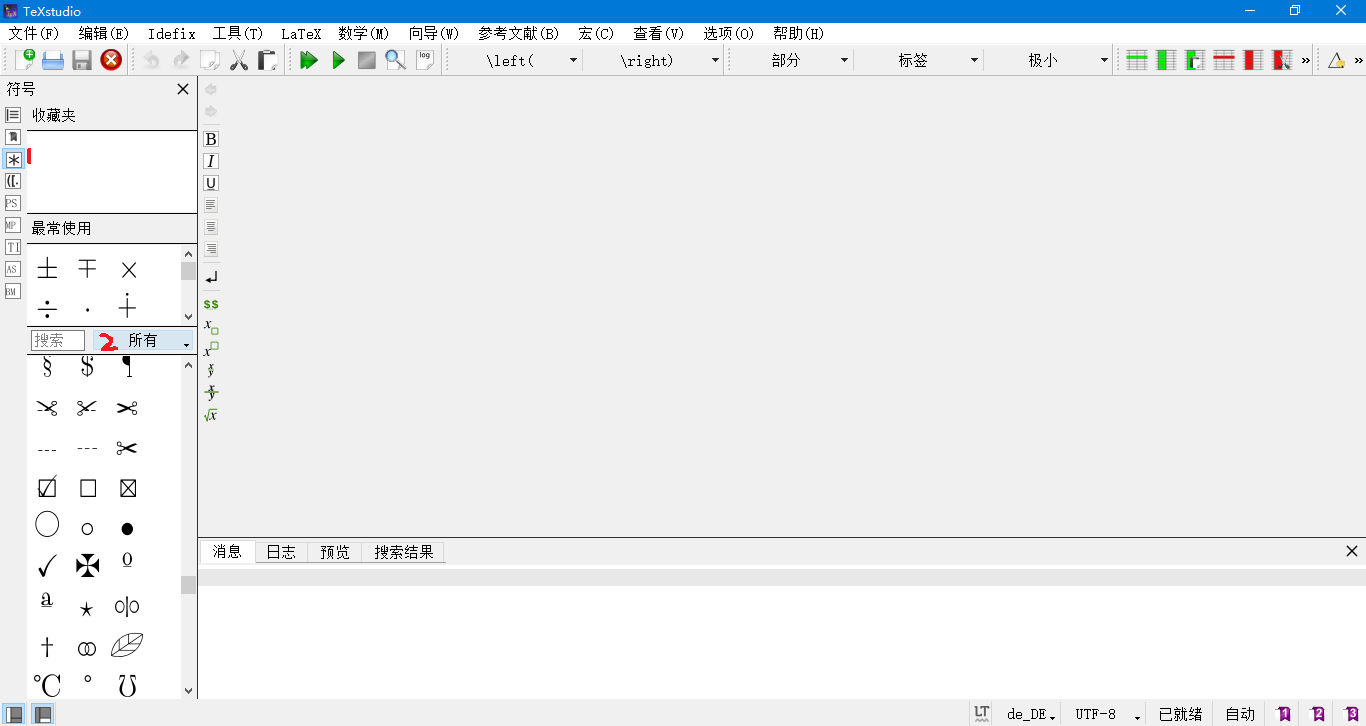
\includegraphics[width=0.9\textwidth]{include/images/5.png}
  \item 也可以手动输入,识别率不是特别高,可能需要多输入几次才会出来。设置如下:向导$\rightarrow$数学助手,手写输入完
  之后插入即可。

  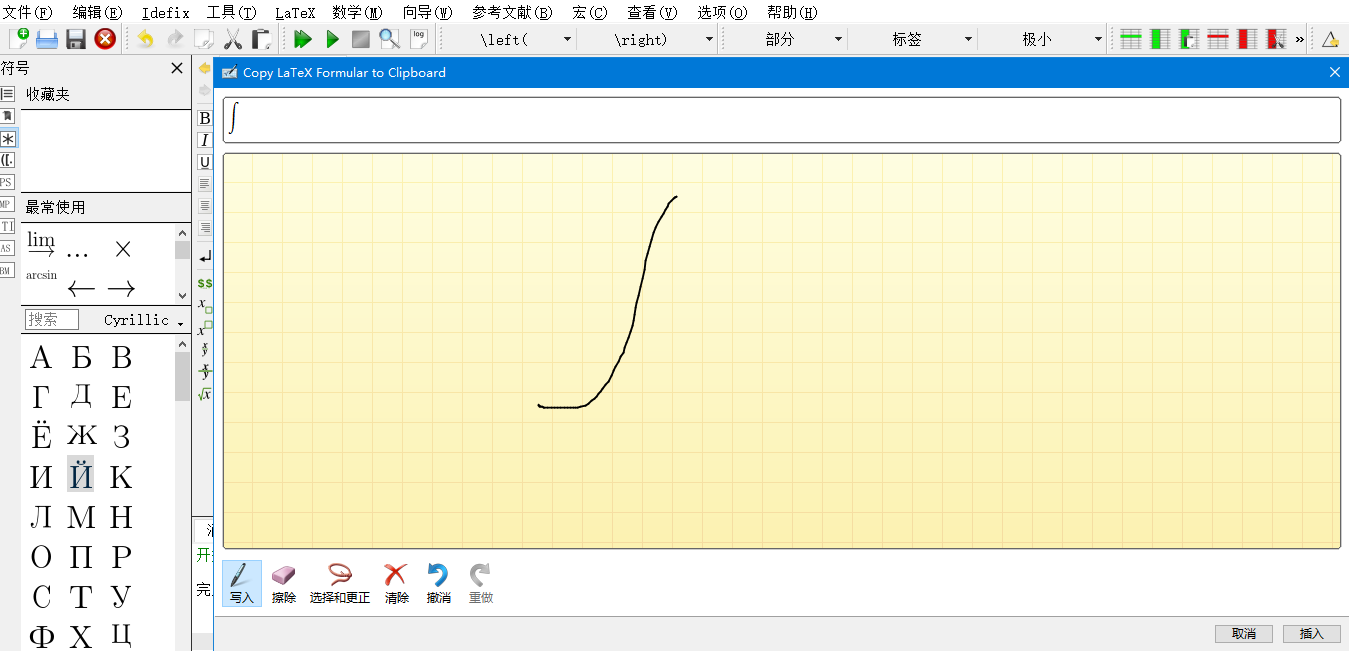
\includegraphics[width=0.9\textwidth]{include/images/image.png}
\end{itemize}


\faq{如何找到 FAQs}{}


\faq{如何控制章节编号的深度}{how-to-control-section-depth}

\LaTeX{} 标准文档类对章节划分了层级:
\begin{itemize}
  \item 在 article 文档类里 part 为0,section 为1,依此类推;
  \item 在 report/book 文档类里 part 为 $-1$,chapter 为0,section 为1,等等。
\end{itemize}

secnumdepth 计数器控制章节编号的深度,如果章节的层级大于secnumdepth,那么章节的标题、在目录和页眉页脚的标题都不编号
(照常生成目录和页眉页脚),章节计数器也不计数。可以用 |setcounter| 命令设置 secnumdepth 为较大的数使得层级比较深的
章节也编号,如设置为4令 |paragraph| 也编号;或者设置一个较小的数以取消编号,如设置为-1 令 |chapter| 不编号。
后者是生成不编号的章节的一个妙招,免去了手动使用 |addcontentsline| 和 |markboth| 的麻烦。
secnumdepth 计数器在 article 文档类里默认为3(subsubsection一级);在 report 和 book 文档类里默认为
2(subsection 一级)。

下面给出一个具体的例子:

\begin{texcode}
  \documentclass{book}
  \setcounter{secnumdepth}{4}
  \begin{document}
    \part{Part}
    \chapter{Chapter}
    \section{Section}
    \subsection{Subsection}
    \subsubsection{Subsubsection}
    \paragraph{Paragraph}
  \end{document}
\end{texcode}

控制目录页排版显示深度可以使用 |\setcounter{tocdepth}{2}|,此命令表示显示到三级标题。关于此问题的具体介绍可以参考
\href{https://blog.csdn.net/RobertChenGuangzhi/article/details/50480856}{该网页}。


\faq{如何下载 arXiv 上面的 \TeX{} 源文件}{how-to-download-arxiv-tex}
先访问 arXiv 上面的文章,在右边找到 Downloads $\rightarrow$ Other formats,点击进入下载页,点击 Download source。
将文件下载到本地后,重命名文件,文件后缀名是 .tar.gz。接下来解压缩 .tar.gz 文件,即可获得 \TeX{} 源文件。


\faq{Windows 系统下用 TeXstudio 打开中文编写的源文件遇到乱码怎么办}{windows-texstudio-chinese-GBK}

最简单的方法是借助 Notepad++ 等编辑器将文件转码为 UTF-8。如果没有 noteapd++,也可以直接使用 TeXstudio。
这里我们默认文件的编码是 GB2312。首先打开文件,在 TeXstudio 右下角找到 encoding 位置的内容,
有时系统显示为 ISO-8859-1。点击那里,进入 More encodings,在列表中点击 GB2312,然后点击按钮 view with。
正常来讲,乱码应该都会消失。 接下来,继续进入 More encodings,在列表中点击 UTF-8,然后点击按钮 change to。
经过这些操作,源文件就重新变成了 UTF-8 编码。


\faq{如何在listing抄录环境中显示公式}{how-to-listing-show-equations}

有时对抄录环境中的代码进行说明时,要用显示公式,这时只要进选项texcl设为true即可。

\begin{verbatim}
  \begin{lstlisting}[
    numbers=left,
    upquote=true,
    basicstyle=\ttfamily,
    texcl=true,
    language=Python
    ]
    #Generates Graphs $G^{(12)} ---  G^{(17)}$
    sGL6=['E@QW', 'EHQW', 'E@`w', 'E@]o', 'E@Rw', 'EAMw']
    GL=[Graph(s) for s in sGL6]
    \end{lstlisting}
\end{verbatim}
%  
%  % \begin{figure}
%  % \centering
%  % \includegraphics{https://images-cdn.shimo.im/LttXT6sECbcak9Qi/image.png!thumbnail}
%  % \caption{图片}
%  % \end{figure}
%  

或者设置mathescape~选项为true。

\begin{verbatim}
  \begin{lstlisting}[mathescape=true]
    if foo
    list= { $S_1,S_2,S_3$ }
  \end{lstlisting}
\end{verbatim}


\faq{能不能介绍一下排版试卷的方法与技巧,比如选择题,密封线设置等。}{how-to-latex-papers}


\faq{一个文档,如何在不同部分使用不同的页眉页脚}{how-to-set-different-geometry}

参考 geometry 宏包的自定义命令。比较常用的有如下四个命令
\begin{verbatim}
  \newgeometry{<options>}
  \restoregeometry
  \savegeometry{<name>}
  \loadgeometry{<name>}
\end{verbatim}
具体可参见该宏包的说明文档。


\faq{如何给中文文本加注音符号?}{how-to-pinyin}

xpinyin 宏包。


\faq{在book类文档中边注用什么宏包?边注的宽度能调整吗?}{book-geometry}


\faq{如何使用ctex相关类或者宏包制定章节样式,目录样式?}{ctex-tableofcontents}


\faq{如何给章节标题,目录列表加盒子边框?}{}


\faq{如何使用带圈数字?}{how-to-use-circle-number}

\begin{verbatim}
  \begin{enumerate}
    \def\labelenumi{\arabic{enumi}.}
    \setcounter{enumi}{7}
\end{verbatim}


\faq{如何改变列表标签样式,行距,缩进等各种相关间距?}{how-to-change-list-style}

enumitem 宏包


\faq{换行与换段的区别,有几种方式?}{change-line-paragraph}

换行是 |\\| 换段是 |\par|,或者空一行。
换行与分段最大的区别在于语义上是否形成一段完整的阐述、叙述,多读两遍你写的文字,如果你觉得问题没有叙述完,那么应该用换行,
反之则应该用分段。


\faq{在使用较早版本的CTeX里面附带的WinEdt出现打不开UTF-8编码文档的情况,如何处理?}{early-version-ctex-winedit-utf8}

使用记事本之类文本编辑器打开,转换编码方式另存一份即可。有时候需要注意BOM问题,一般没啥问题。


\faq{如何改变计数器样式为中文数字、罗马数字、阿拉伯数字或拉丁字母?}{how-to-change-listing-number}

可以通过重定义命令的方式修改默认的计数器样式,例如
\begin{verbatim}
  \renewcommand{\thechapter}{\Roman{chapter}}
\end{verbatim}
会将章序号计数器改为大写罗马数字计数形式。更多对应关系如下所示:

\begin{table}[h]
  \centering
  \begin{tabular}{cc}
    |\arabic| & 阿拉伯数字 \\
    |\alph| & 小写英文字母,数值应小于27 \\
    |\Alph| & 大写英文字母,数值应小于27 \\
    |\chinese| & 中文小写数字,需要调用\CTeX{}宏包 \\
    |\roman| & 小写罗马数字 \\
    |\Roman| & 大写罗马数字 \\
    |\fnsymbol| & 脚注标识符,数值应小于10
  \end{tabular}
\end{table}

详情可以参阅刘海洋、胡伟等编写的相应书籍,也可以查阅Wiki百科。


\faq{列表环境 (enumerate/itemize/description)的条目间距太大了,怎么改小一些?}{how-to-change-listing-linespace}

可以使用 paralist 宏包,它提供了一系列压缩了行间距的列表。对应的环境名称分别是 compactenum/compactitem/compactdesc,
也可以使用 enumitem 宏包修改三个列表环境的格式。


\faq{列表的条目项内容很短,可以让他们在一行内排版么?}{listing-short-oneline}

可以使用 paralist 宏包,这个宏包提供了 inparenum/inparitem/inpardesc 环境,可以在行内输出列表内容;
也可以带上 inline 选项使用 enumitem 宏包,可以使用带*形式的三个列表环境,即在行内输出列表内容。


\faq{enumerate宏包修改列表标签格式很方便,但是这个宏包和enumitem宏包冲突,有什么解决办法么?}{enumerate-fight-enumitem}

如果只是需要使用这种短标签表示方法,利用enumitem宏包同样能够做到,只需要带上shortlabels选项加载enumitem宏包即可。
同时,enumitem宏包提供了自定义短标签名称和格式的宏命令,你也可以自己定义一些有趣的标签形式。


\faq{如何使用带圈数字作为 enumerate 列表的标签?}{circle-number-enumerate}

\LaTeX{} 自带一个带圈字符的命令 |\textcircled|,不过,这个命令的排版效果非常差,几乎很少有人会直接使用。
带圈数字可以通过unicode字符实现,也可通过pifont宏包中|ding|命令实现(但是只能用到10以内的数字),
甚至可以通过tikz 自己绘制一个。使用带圈数字做enumerate的标签,可以通过 enumitem 宏包设置。
这里给出一个使用 unicode 字符实现带圈数字的方法,并将其应用于enumerate 的标签。

\begin{verbatim}
  \documentclass{article}
    \usepackage{xeCJK,xunicode,calc}
    \usepackage[shortlabels]{enumitem}
    \newcommand{\Cnum}[1]{%
    \ifnum #1<21
      \edef\a{\the\numexpr #1+9311}
    \else
      \ifnum #1<36
        \edef\a{\the\numexpr #1+12860}
      \else
        \ifnum #1<51
         \edef\a{\the\numexpr #1+12941}
        \else
          \PackageError{your package}{Number too large}{}
        \fi
      \fi
    \fi
    {\CJKfontspec{Noto Serif CJK SC}\fontspec{Noto Serif CJK SC}\symbol\a}}
    \SetEnumerateShortLabel{o}{\protect\Cnum{\arabic*}}
    \begin{document}
    \Cnum{12} \Cnum{32} \Cnum{46} 
    
    \begin{enumerate}[o]
      \item The first item.
      \item The second item.
      \item The Third One.
    \end{enumerate}
    \end{document}
\end{verbatim}


\faq{如何给目录中的章节都带上引导点来连接页码?}{tableofcontents-dotdotdot}

其实级别较高的章节结构,如book/report中的chapter和arcticle中的section,是不需要这种引导点来连接页码的,有这种需求
的多是受Microsoft Word的影响。如果一定要这种引导点,可以在导言区增加这样一段代码。
\begin{verbatim}
  \makeatletter
  \def\@bfdottedtocline#1#2#3#4#5{%
  \ifnum #1>\c@tocdepth \else
  \vskip \z@ \@plus.2\p@
  {\leftskip #2\relax \rightskip \@tocrmarg \parfillskip -\rightskip
  \parindent #2\relax\@afterindenttrue
  \interlinepenalty\@M
  \leavevmode \bfseries
  \@tempdima #3\relax
  \advance\leftskip \@tempdima \null\nobreak\hskip -\leftskip
  {#4}\normalfont\nobreak
  \leaders\hbox{$\m@th
  \mkern \@dotsep mu\hbox{.}\mkern \@dotsep
  mu$}\hfill
  \nobreak
  \hb@xt@\@pnumwidth{\hfil\normalfont \normalcolor #5}%
  \par}%
  \fi}
  \renewcommand*\l@section{\@bfdottedtocline{0}{0em}{1.5em}}
  \makeatother
\end{verbatim}
当然,最后一句应根据实际的文档类型来重定义 |\l@chapter| 或 |\l@section|。


\faq{如何临时切换页面大小?}{}


\faq{没有编号的章节标题如何添加到目录里?}{no-number-chapter-tableofcontents}

使用 |\addcontentsline{toc}{<level>}{<title>}|;举个例子:
\begin{verbatim}
  \section*{译者序}\addcontentsline{toc}{section}{译者序}
\end{verbatim}
这样在目录中译者序是没有编号的,对应等级是section,标题是译者序。参考:《lshort》目录章节。


\faq{怎样定义“第几页/共几页”的页码样式?}{how-to-define-pagenumber}

可以调用末页标签宏包 lastpage,并将页码设置如下:
\begin{verbatim}
  第 \thepage 页 / 共 \pageref{LastPage} 页
\end{verbatim}

如果不想调用这个宏包,还可以自己DIY,虽然ugly,但是可以达到目的 ):在文档末尾设置一个标签,
例如在 |\end{doucument}| 前加一句 |\label{AllPage}|,然后将页码设置为:
\begin{verbatim}
  第 \thepage 页 / 共 \pageref{AllPage} 页
\end{verbatim}


\faq{超链接如何断行?}{url-how-to-multilines}

先写
\begin{verbatim}
  \PassOptionsToPackage{hyphens}{url}
\end{verbatim}

再写
\begin{verbatim}
  \usepackage{hyperref}
\end{verbatim}


\faq{如何在axmath转换代码到TeXstudio?}{how-to-axmath-exchange-to-texstudio}

点击下图中第10个按钮,即可将数学公式转换为\LaTeX{}代码,复制即可。


\includegraphics[width=0.9\textwidth]{include/images/amxmath_texstudio}


\faq{双栏文档中,如何可以让左边先写完,然后再切换到右边,而不是左右一样长?}{twocolumn-left-first}

如果是采用文档类 twocolumn 选项实现的双栏模式,正文的排版就是先将左边排完,再从右边开始排。而采用
multicol 宏包的 muticols 环境则是左右两边底部对齐的。 


\faq{如何输入中文破折号?}{input-chinese---}

输入法输入咯,英文的破折号 --- 用于中文不合适。


\faq{input和include有何区别?}{input-include-difference}

\begin{itemize}
  \item |\include| 在读入文件之前会另起一页。|\input| 命令纯粹是把文件里的内容插入
  \item |\include| 不可用于导言区,而且导言区使用了 |\includeonly| 命令后,
  |\include| 仅会引入由 |\includeonly| 指定的文件。
  \item |\include| 引入的文件中,不可以再次使用 |\include| 命令。
\end{itemize}


\faq{subfiles有什么用?}{subfiles-usage}

详细功能可以查看此宏包自带的文档。编辑由一个主文档若干个子文档构成的多文档项目时使用此宏包会更方便。用户可以正常编译使用
|\input| 导入子文档的主文档,也可以直接编译子文档本身,此时子文档使用跟主文档相同的导言区而成为完整的一份\TeX{}文档。


\faq{如何使用latexmk编译文档?}{}


\faq{定理环境要怎么使用?}{}


\faq{算法环境如何使用?}{}


\faq{在lstlisting环境中如何输出破折号?}{}


\faq{minted里面Tab键为什么会输出成\^{}\^{}T,如何解决?}{}


\faq{一段代码粘贴到TeXstudio里面就没有了缩进,如何解决?}{}


\faq{在\LaTeX{}或Tikz中,能否输入随机且字数随机可控的文字?}{}


\faq{如何输入罗马数字等?}{how-to-input-roman-numbers}

一种方式是定义宏显示罗马数字,代码如下:
\begin{verbatim}
  \newcommand{\Myroman}[1]{\romannumeral #1}
  \newcommand{\MyRoman}[1]{\expandafter\@slowromancap\romannumeral #1@}
\end{verbatim}
正文中使用
\begin{verbatim}
  \MyRoman{3} \Myroman{5}
\end{verbatim}

另一种投机取巧的方式是你可以先定义一个counter,然后给这个counter的数值设置成需要表达的数值,
再用 |\Roman| 或 |\roman| 显示这个计数器。举例如下:
\begin{verbatim}
  \newcounter{romannum}
  \newcommand{\MyRoman}[1]{\setcounter{romannum}{#1}\Roman{romannum}}
  \newcommand{\Myroman}[1]{\setcounter{romannum}{#1}\roman{romannum}}
\end{verbatim}
使用方法相同。


\faq{如何在等号中插入问号?}{how-to-input-.-in-questionmark}

\begin{verbatim}
  \stackrel{?}{=}
\end{verbatim}


\faq{如何在插入的图片上标记引注?}{input-mark-in-pictures}

可以看看overpic之类的宏包。


\faq{如何让一个很长很长的字符串(中间不带空格)自动换行?}{how-to-disable-long-string-multilines}

了解下分词断行机制就不会有此问题了。


\faq{\cs{bf}、\cs{sf}、\cs{it}、\cs{sl}这些命令都很短小,为什么不建议继续使用了?}{}


\faq{如何自动化打包 \LaTeX{} 文档发送给别人以确保宏包、字体是完整的,便于他人顺利编译、减少麻烦。}{}


\faq{如何编译网站上下载的他人的模板,一般是不知道对应的编译器应该选择什么,还有编译顺序是什么,
希望在提供模板的同时说明应该如何编译。}{}


\faq{我以book文档类为基础新写一个文档类,book文档类的选项会自动适用于我新建的文档类么?}{}


\faq{\cs{def} 和 \cs{newcommand} 有什么区别,我创建新命令的时候究竟应该用哪个?}{}


\faq{怎样创建一个带*的命令?}{newcommand-with-*}

有以下几种方法:
\begin{itemize}
  \item 最基本的方法,使用 \LaTeX{} 内部命令 |\@ifstar| 判断
  \begin{verbatim}
    \makeatletter
    \newcommand{\mycommand}{%
      \@ifstar
        \mycommandStar%
        \mycommandNoStar%
    }
    \makeatother
    \newcommand{\mycommandStar}{starred version}
    \newcommand{\mycommandNoStar}{normal version}
  \end{verbatim}
  \item 比较简单的方法,使用 ifthen 宏包
  \begin{verbatim}
    \usepackage{ifthen}
    \newcommand{\mycommand}[1]{\ifthenelse{\equal{#1}{*}}%
      {\mycommandStar}%
      {\mycommandNoStar{#1}}%
    }
    \newcommand{\mycommandStar}{starred version}
    \newcommand{\mycommandNoStar}[1]{normal version}  
  \end{verbatim}
  \item 使用\LaTeX{3}的机制
  \begin{verbatim}
    \usepackage{xparse}
    \NewDocumentCommand\mycommand{s}{%
      \IfBooleanTF#1%
        {starred version}%
        {normal version}%
    }
  \end{verbatim}
\end{itemize}


\faq{类似 \cs{macro[<option1>][<option2>]\{<arg>\}} 这样的宏命令,当我只使用一个可选参数时,\LaTeX{}把它看做哪个参数?\LaTeX{}会自动判断么?}{}


\faq{\cs{newcommand} 创建的命令,仅有第一个命令可以成为可选参数,如果我想创建具有两个可选参数的命令,应该如何去写?}
{newcommand-multi-optional}

可以用一个小把戏实现:
\begin{verbatim}
  \newcommand{\mycmd}[1][option1]{%
    \def\ArgI{{#1}}%
    \mycmdoptii
  }
  \newcommand\mycmdoptii[1][option2]{%
    ...
  }
\end{verbatim}

或者使用\LaTeX{3}的机制:
\begin{verbatim}
  \usepackage{xparse}
  \NewDocumentCommand\mycmd{O{option1} O{option2} m}{%
    #1#2#3
  }
\end{verbatim}


\faq{有些命令的参数是使用 () 扩起来的,这类命令是如何定义的?}{}


\faq{我想新建一个带有可选参数的命令,可选参数的缺省值与必选参数值一样,这样的命令如何创建?}{}

第一种方法:
\begin{verbatim}
  \newcommand{\mycmd}[2][\DefaultOpt]{%
    \def\DefaultOpt{#2}%
    optional arg: #1,  mandatory arg: #2%
  }
\end{verbatim}

第二种方法:
\begin{verbatim}
  \def\mycmd{\futurelet\testchar\WithOptCmd}
  \def\WithOptCmd{%
    \ifx[\testchar 
      \let\next\OptCmd 
    \else 
      \let\next\NoOptCmd 
    \fi\next}
  \def\OptCmd[#1]#2{optional arg: #1,  mandatory arg: #2}
  \def\NoOptCmd#1{optional arg: #1,  mandatory arg: #1}
\end{verbatim}


\faq{想用minted包写文档,怕别人用不来不会设置-shell --escepe咋办}{}

教给别人怎么用,或者不用这个宏包。


\faq{如何给整个页面加边框?}{}


\faq{每一部分第一段段首如何空两格,区别于下面段落的自动换行。}{}

使用 |\usepackage{indentfirst}|


\faq{如何在section中使用box}{}


\faq{\cs{lstinputlisting}在\XeLaTeX{}下如何支持中文?}{}


\faq{Excel里的矢量图怎么存为eps并插入\TeX{}中?\& Matlab 导出图片无白边?}{}


\faq{如何结合使用 Pandoc 和 \LaTeX{},提高文档编写效率?(或如何结合使用 Markdown 和 LaTeX?)}{}


\faq{\cs{label\{key\}}可以用中文吗,如\cs{label\{第一章\}}}{}


\faq{如何将算法代码的行编号放到外边框的里面?}{}


\faq{如何编辑页眉和页脚,添加页码}{}


\faq{\LaTeX{}写毕业论文时,直接写编译速度慢,用dvi会不会简便些?}{}


\faq{文字用 \cs{underlined} 加了下划线后为什么没法换行?}{}


\faq{如何使用带圈数字做脚注编号?}{}


\faq{怎样判断当前页是奇数页还是偶数页?}{}


\faq{如何加粗Listing中的一行文本?}{}


\faq{如何根据不同的编译引擎选择执行不同的宏命令?}{}


\faq{我怎么能把页码改成以三位数字(前导的0也显示出来)表示?}{}


\faq{標點符號如何分類設置樣式?比如逗號、句號、頓號等設爲一類,歎號、問號設爲一類,引號、書名號設爲一類,等等。}{}


\faq{请问交叉引用用\cs{ref\{\}}引用的表格,图片,在PDF上点击数字时没有反应,不能跳转到相应的表格、图片位置,
生成的目录点击时也跳转不到指定的页码,在书上没有查到原因,我用的\TeXLive{} 2017+TeXstudio,是设置的问题还是其他问题?}{}



% Copyright (C) 2018 by latexstudio <http://www.latexstudio.net>
%
% This program is free software: you can redistribute it and/or modify
% it under the terms of the GNU General Public License as published by
% the Free Software Foundation, either version 3 of the License, or
% (at your option) any later version.
%
% This program is distributed in the hope that it will be useful,
% but WITHOUT ANY WARRANTY; without even the implied warranty of
% MERCHANTABILITY or FITNESS FOR A PARTICULAR PURPOSE.  See the
% GNU General Public License for more details.
%
% You should have received a copy of the GNU General Public License
% along with this program.  If not, see <http://www.gnu.org/licenses/>.
%

% !TEX root = ../latex-faq-cn.tex
% !TEX program = xelatex
% !TEX options = --shell-escape

\let\fancybreak\relax

\section{数学公式(一)}
\label{sec:math-i}

%TODO: General

\faq{不带编号的行间公式为什么推荐使用 \cs{[}\ldots\cs{]} 而不是
  \texttt{\$\$}\ldots\texttt{\$\$}?}{display-math-env}

|$$|\ldots|$$| 是 \TeX{} 的用法,不适合在 \LaTeX{} 中使用。在 \LaTeX{} 中,\cs{[}\ldots\cs{]} 虽然
底层仍然依靠 |$$|\ldots|$$| 实现,但显然更加容易控制,也更容易实现特殊效果(例如靠左对齐)。

在 \pkg{amsmath} 宏包中,\cs{[}\ldots\cs{]} 被重定义为 \env{equation*} 环境的简写,它的实现比
\LaTeX{} 本身更好。所以我们建议,排版数学公式时始终调用 \pkg{amsmath} 宏包。

\begin{reference}
  \item 李清.\LaTeX{} 中不带编号的行间公式为什么推荐用 \cs{[}\ldots\cs{]} 而不是 |$$|\ldots|$$|?.
    \url{https://www.zhihu.com/question/27589739/answer/37255728}
  \item \url{https://tex.stackexchange.com/q/503}
  \item \url{https://tex.stackexchange.com/q/40492}
\end{reference}


\faq{如何让长公式自动断行?}{break-long-equation}

对于行内公式,一般来说 \LaTeX{} 会倾向于在二元运算符($+$、$-$ 等)和二元关系符($=$、$>$ 等)之后
断行,因此可以用 $F(x) \cdot G(x) \cdot H(x)$ 来代替 $F(x)G(x)H(x)$ 以允许换行。另外,我们建议把
列表项写成如 |$a$, $b$, $c$| 的形式而非 |$a, b, c$|,这样也可以避免出现糟糕的效果。

对于行间公式,可以使用 \pkg{amsmath} 宏包提供的一系列环境来手动断行:
\begin{itemize}
  \item \env{gather} 和 \env{gather*}:居中对齐
  \item \env{align} 和 \env{align*}:在 |&| 指定的位置对齐
  \item \env{multiline} 和 \env{multiline*}:首行左对齐,末行右对齐,中间居中
  \item \env{split}:类似 \env{align},在 |&| 指定的位置对齐,但需放在其他数学环境中使用
\end{itemize}
这里带 |*| 的版本表示不加编号。以上这些环境用法都是类似的,即在断行处加 |\\|。

公式的断行往往需要考虑语义因素,需要正确处理间距、对齐等,因此自动断行比较困难。\pkg{breqn} 宏包
提供了自动断行的可能,但有时候会出现兼容性问题,需要小心使用。

\begin{reference}
  \item 刘海洋.《\LaTeX{} 入门》 4.4~节、4.5.3~小节
\end{reference}


\faq{公式如何靠左(靠右)对齐?}{equation-left-right-align}

公式靠左对齐在基础文档类中由 |fleqn| 选项控制。选择该选项后,正文公式均靠左对齐,并且具有固定缩进
(由 \cs{mathindent} 控制)。至于(全局)靠右对齐,并没有直接的解决方案。

如果只需要部分公式靠左或靠右对齐,可以用 \env{flalign} 或者 \env{flalign*} 环境:

\begin{texlist}
  \begin{flalign}
    \int \sin x \, \mathrm{d} x = -\cos x + C & &
  \end{flalign}
  \begin{flalign}
    \int \cos x \, \mathrm{d} x = \sin x + C & &
  \end{flalign}
  \begin{flalign}
    & & \int \tan x \, \mathrm{d} x =  \ln |\sec x| + C
  \end{flalign}
\end{texlist}

\env{flalign} 环境本身用来实现分散对齐。因此用 |&&| 构成空列,就可以实现靠左或靠右对齐的效果:
\begin{flalign}
  \int \sin x \, \mathrm{d} x = -\cos x + C & &
\end{flalign}
\begin{flalign}
  \int \cos x \, \mathrm{d} x = \sin x + C & &
\end{flalign}
\begin{flalign}
  & & \int \tan x \, \mathrm{d} x =  \ln \vl\sec x\vl + C
\end{flalign}

\begin{reference}
  \item \url{https://tex.stackexchange.com/q/16840}
\end{reference}


\iffalse


\faq{公式希腊字符如何加粗?}{}

希腊字母没有原生粗体,可以使用 \pkg{bm}宏包中的|\bm|命令,
或者\pkg{unicode-math}宏包\footnote{需指定OpenType Math font,源代码文字为UTF8编
  码,直接输入希腊文。此包不能与其他一些math包共存。}中的|\symbol{AaBb∇αβγ}|或者其他伪粗命令。
粗。
\begin{reference}
  \item stackexchange. How can I get bold math symbols?. \url{https://tex.stackexchange.com/questions/595/how-can-i-get-bold-math-symbols}
\end{reference}


\faq{极限符号下面有两个趋近该怎么写}{}

直接给出例子:

%\begin{verbatim}
\begin{example}
\[ \lim_{n\to\infty\atop m\to\infty} \]
\end{example}
%\end{verbatim}
%效果如下:
%
%\[ \lim_{n\to\infty\atop m\to\infty} \]
%\begin{Example}
%	\[ \lim_{n\to\infty\atop m\to\infty} \]
%\end{Example}

%\begin{example}
%	$\frac{1}{\pi}$,\quad
%	$\sqrt[5]{1+k^2+k^4}$
%\end{example}

%\begin{Example}
%	$\frac{1}{\pi}$,\quad
%	$\sqrt[5]{1+k^2+k^4}$
%\end{Example}

或者使用 \cs{substack},代码如下:

%\begin{texlist}
%\documentclass{article}
%\usepackage{amsmath}
%\begin{document}
%\[ \lim_{\substack{n\to\infty\\ m\to\infty}} \]
%\end{document}
%\end{texlist}
%
%效果如下:
%
%\[ \lim_{\substack{n\to\infty\\ m\to\infty}} \]
\begin{example}
\[ \lim_{\substack{n\to\infty\\ m\to\infty}} \]
\end{example}
 
% \includegraphics{https://images-cdn.shimo.im/FCY4A1SeBIcwBCGT/双重极限.PNG!thumbnail}


\faq{怎样在 LaTeX 中输入引号}{}

左引号用 `(键盘1旁边那个键),右引号用 `。西文双引号使用``''。
中文条件下应直接使用中文双引号。
\begin{reference}
  \item 中华人民共和国教育部. 夹用英文的中文文本的标点符号用法(草案).\url{http://www.moe.gov.cn/s78/A19/yxs_left/moe_810/s230/201001/t20100115_75604.html}
\end{reference}


\faq{align环境默认是居中对齐吗?我在使用时,发现公式开始是居中的,后来却一直靠右断对齐,这是什么原因?}{}

align采用的是奇偶对齐的方式,第一列右对齐,第二列左对齐,就这样右左右左依此类推,
两列之间用\&分隔。


\faq{中英文标点使用规则不是很明白,尤其在公式环境里,字体和间距差别都比较大。怎样才能让正文和公式的标点统一(形状和间隔)?}{}

详见:
\url{https://link.zhihu.com/?target=http\%3A//www.moe.gov.cn/ewebeditor/uploadfile/2015/01/13/20150113092346124.pdf}

在导言区加类似命令可实现全文替换:

\begin{texlist}
\catcode`\。=\active\newcommand{。}{. }
\end{texlist}

或者使用 xeCJK 宏包的字符映射功能,调用 fullwidth-stop
这一映射文件,将中文空心句号映射为实心句点:

\begin{texlist}
\documentclass{article}
\usepackage{xeCJK}
\setCJKmainfont[Mapping= fullwidth-stop]{STSong}
\begin{document}
句号。
\end{document}
\end{texlist}


\faq{公式之后解释公式符号的文字,通常是 ``符号 ------ 解释'' 这样的格式,我希望这段文字的格式是按破折号对齐,并且解释文字折行后悬挂缩进,怎样实现这样的格式?}{}

方法很多,可以列表,可以align等环境。 这里给出一个使用自定义列表的例子:

\begin{texlist}
\usepackage{ifthen}
\newcounter{qlst}
\newenvironment{EqDesc}[2][式中]{%
\begin{list}{}
 {%
  \usecounter{qlst}
  \settowidth{\labelwidth}{#1,\ \ #2\ --- \ }
  \setlength{\labelsep}{0pt}
  \setlength{\leftmargin}{\labelwidth}
  \setlength{\rightmargin}{0em}
  \setlength{\parsep}{0ex}
  \setlength{\itemsep}{0ex}
  \setlength{\itemindent}{0em}
  \setlength{\listparindent}{0em}
  \renewcommand{\makelabel}[1]
    {\stepcounter{qlst}
     \ifthenelse{\value{qlst}>1}{\hfill ##1\ --- \ }{#1,\hfill ##1\ --- \ }
    }
 }%
}%
{\end{list}}
\end{texlist}

EqDesc
环境有两个参数,第一个为可选参数,是解释公式符号前的引导词,默认是``式中'',第二个参数是样本符号,可以选择一个列表中宽度最大的符号。条目 \cs{item} 有一个可选参数(实际使用是必选参数),内容是要说明的符号。使用如下:

%\begin{verbatim}
\begin{example}
\[ a^2+b^2=c^2 \]
\begin{EqDesc}[其中]{$a$}
   \item[$a$] 三角形的一条直角边;
   \item[$b$] 三角形的另一条直角边;
   \item[$c$] 三角形的斜边。
\end{EqDesc}
\end{example}
%\end{verbatim}

%{\centerline{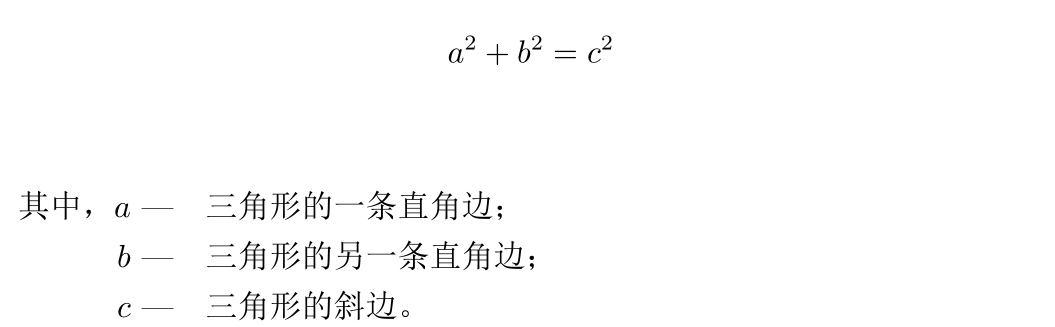
\includegraphics[width=0.8\linewidth]{include/images/hang}}}


\faq{行内公式的情况下如何让sum prod这些运算符的上下标在头上和脚下?}{}

这样处理行内公式的上下标会导致段落行距不整齐,不符合 \LaTeX{}
的审美。如果彻底放弃审美,可以使用 \cs{limits} 命令,如:

%\begin{verbatim}
\begin{example}
$\sum\limits_{i=1}^n, \prod\limits_\epsilon$
\end{example}
%\end{verbatim}

%效果是这样的:$\sum\limits_{i=1}^n \quad \prod\limits_\epsilon$

\faq{如何将积分的上限标放在积分号的上下两侧?}{}

积分号的上下限放置在积分号的右侧是英美国家和 \LaTeX{}
的排版习惯,通常无需处理。
如果你很确定需要按照 ISO 80000-2:2009 或者 GB 3102.11-93 的规定排版积分号,可以:

\begin{enumerate}
\def\labelenumi{\arabic{enumi}.}

\item
  在调用 amsmath 宏包时添加 intlimits 选项;
\item
  \texttt{\cs{def}\cs{int}\{\cs{intop}\}}
\item
  如果使用 unicode-math 宏包,
\end{enumerate}

\begin{texlist}
\removenolimits{%
  \int\iint\iiint\iiiint\oint\oiint\oiiint
  \intclockwise\varointclockwise\ointctrclockwise\sumint
  \intbar\intBar\fint\cirfnint\awint\rppolint
  \scpolint\npolint\pointint\sqint\intlarhk\intx
  \intcap\intcup\upint\lowint
}
\end{texlist}


\faq{如何自定义数学运算符,然后让下标放在脚下?}{}

借助 amsmath 包(实际上是amsmath自动调用的amsopn宏包)的
\cs{DeclareMathOperator*} 命令,可以在导言区定义需要的数学运算符(需要注意加不加*是有区别的)。例如

\begin{texlist}
\DeclareMathOperator*{\esssup}{ess\,sup}
\end{texlist}

\begin{example}
\[ 
  \esssup_{x\in {R}} 
\]
\end{example}


对于只是偶尔用到的运算符,也可以无需定义而直接在数学模式中使用新算符定义命令。
%
%例如
%|\operatorname*{ess\,sup}_{x\in {R}}|

\begin{example}
\[
  \operatorname*{ess\,sup}_{x\in {R}}
\]
\end{example}


\faq{行列式变换过程中,我们一般是在中间的箭头上表示出变换的方式,如何才能在长箭头上打出多行内容?}{}
可以看看amsmath宏包提供的长箭头命令。
\begin{example}
\[
  A \xleftarrow[formula-1]{formula-2} B,
  C \xrightarrow[formula-1]{formula-2} D
\]

\end{example}

\faq{如何输出反斜杠?}{}
方式很多,例如
\begin{example}
  \textbackslash \quad 或者 \quad \verb|\|
\end{example}
%
%\begin{texlist}
%    \textbackslash 或者 \verb|\|
%\end{texlist}


\faq{对equation环境下的公式、图片编号按章节、小节进行重新定义}{}

公式编号使用amsmath宏包的numberwithin设定关联即可。
图片编号可以使用caption宏包自定义格式。

\faq{带括号的公式有哪些折行方式?在括号中间折行。}{}
使用| \left( \right) |括起来的内容不能直接折行,但是可以变通,比如使用| \left( | 匹配 | \right. | 和 | \left. | 匹配 | \right) |,
这时候需要借助幻影、支柱等方法处理各行内容高度不同带来的括号大小不同问题。

\faq{怎么在极限符号下面打出x→0 }{}
很简单的基本指令就行,例如|\lim\limits_{x \to 0}|得到$\lim\limits_{x \to 0}$
\begin{example}
\[
  \lim\limits_{x \to 0}
\]
\end{example}

\faq{\LaTeX{}敲的公式可以插入word吗?}{}
可以,但是不推荐。

\faq{公式中的文本怎么输入?}{}
公式中的文本输入,可以用 \verb|\mbox{...}|。使用率较高的是 \texttt{amstext} 宏包中提供了\verb|\text|命令,示例如下:
\begin{example}
\begin{center}
  This is $_{\text{subscript}}$\\
  This is $_{\mbox{subscript}}$
\end{center}
\[a = b, \text{\qquad by assumption}\]
\end{example}

%\begin{note}\small \itshape
	我们加载 amsmath 宏包的时候,系统会自动调用amstext, amsbsy, amsopn,
	amsintx包,所以无需我们额外加载包。
%\end{note}
%\begin{note}
%	\small \itshape

 这里需要注意的是若是我们的文本部分与其他字符有间隔,需要在\verb|\text{}|里面进行添加。
%\end{note}
%\fancybreak
\faq{如何输入连分数?}{}
\verb|amsmath| 宏包提供的命令 \verb|cfrac| 用于排版连分数,比我们直接使用 \verb|\frac| 排版的效果要好。如:
\begin{example}
\[
  \cfrac{1}{\sqrt 2 + \cfrac{1}{\sqrt 2 +\dotsb}},\quad
  \frac{1}{\sqrt 2 + \frac{1}{\sqrt 2 +\dotsb}}
\]
\end{example}


\faq{如何输入带方框的公式?}{}


可以使用命令 \verb|boxed| 将公式放在方框中,这个命令类似 \verb|\fbox| 如
\begin{example}
\[
  \boxed{\eta \leq C \text{ and } C \leq \Delta}
\]
\end{example}

另外,\verb|fancybox| 宏包提供的几个环境和命令会把公式的编号和公式一起放在方框中。

\faq{实数域 $\mathbb{R}$ 或复数域 $\mathbb{C}$ 等的字体该用什么命令?}{}
使用 amsfonts 宏包提供的\verb|\mathbb{字母}|命令, 例如:
\begin{example}
 $x \in \mathbb{R}$ and $c \in \mathbb{C}$
\end{example}



通常,排版时有些符号需要特殊字体,这里简单列举常用的几个字体。

%\begin{center}
%\includegraphics{fig2}
%\end{center}

{\small\begin{tabular}{ll}
		\hline
		命令&样例\\
		\hline
		默认&${ABCDEFGHIJKLMNOPQRSTUV WXYZ}$\\
		&${abcdefghijklmnopqrstuvwxyz}$\\
		\verb|\mathit|&$\mathit{ABCDEFGHIJKLMNOPQRSTUV WXYZ}$\\
		&$\mathit{abcdefghijklmnopqrstuvwxyz}$\\
		\verb|\mathbf|&$\mathbf{ABCDEFGHIJKLMNOPQRSTUV WXYZ}$\\
		&$\mathbf{abcdefghijklmnopqrstuvwxyz}$\\
		\verb|\mathrm|&$\mathrm{ABCDEFGHIJKLMNOPQRSTUV WXYZ}$\\
		&$\mathrm{abcdefghijklmnopqrstuvwxyz}$\\
		\verb|\mathsf|&\textsf{ABCDEFGHIJKLMNOPQRSTUV WXYZ}\\
		&\textsf{abcdefghijklmnopqrstuvwxyz}\\
%        |\bm|$^a$ & $\bm{ABCDEFGHIJKLMNOPQRSTUV WXYZ}$\\
%        & $\bm{abcdefghijklmnopqrstuvwxyz}$\\
		\verb|\mathscr|$^a$&{\usefont{U}{rsfs}{m}{n}ABCDEFGHIJKLMNOPQRSTUV WXYZ}\\
		\verb|\mathfrak|$^b$&{\fontencoding{U}\fontfamily{euf}\selectfont ABCDEFGHIJKLMNOPQRSTUV WXYZ}\\
		&{\fontencoding{U}\fontfamily{euf}\selectfont abcdefghijklmnopqrstuvwxyz}\\
		\verb|\mathcal|&$\mathcal{ABCDEFGHIJKLMNOPQRSTUV WXYZ}$\\
		\verb|\mathbb|$^c$&$\mathbb{ABCDEFGHIJKLMNOPQRSTUV WXYZ}$\\
		\hline
%		$^a$ 需要 \verb|bm|宏包&\\
		$^a$ 需要 \verb|mathrsfs|宏包&\\$^b$ 需要 \verb|amsfonts|宏包&\\$^c$ 需要 \verb|amsfonts|宏包&\\
\end{tabular}}

\faq{$n$次根式 $\sqrt[n]{\text{Roots}}$ 的位置调整}{}
通常,我们用 \verb|\sqrt[...]{...}| 来输入公式。
\begin{example}
$\sqrt2$, $\sqrt2y$, $\sqrt{2y}$\\
$\sqrt[3]{2}$, $\sqrt[n+1]{x+y}$
\end{example}

按照如上的输入方式,我们输入如下公式 \verb|$\sqrt[\frac{1}{n}]{a}$| 会输出 $\sqrt[\frac{1}{n}]{a}$ ,而 \verb|$\sqrt[\beta]{a}$| 输出为 $\sqrt[\beta]{a}$。
我们需要这样调整:
\begin{example}
$\sqrt[\leftroot{2}\uproot{4}\beta]{k}$,
$\sqrt[\leftroot{1}\uproot{3}\beta]{k}$,
$\sqrt[\leftroot{2}\uproot{4}\frac{1}{n}]{k}$,
$\sqrt[\leftroot{1}\uproot{3}\frac{1}{n}]{k}$
\end{example}
\noindent 这两个命令 \verb|leftroot| 和 \verb|uproot| 分别表示将方根向左向上移动 $n$ 个单位,若为负数表示向反方向移动。


\faq{如何输入在等号上输入如 def 等文字?}{}

对于这种特殊的重叠符号,可通过使用 \verb|amsmath| 宏包的 \verb|overset|
命令来实现。具体用法见下面的例子。
\begin{example}
\begin{equation}a\overset{?}{=}b\end{equation}
\end{example}

若等号上文字较多时,这时我们可以用 \verb|extarrows| 宏包的自适应长度的等号,简单示例如下:
\begin{example}
\begin{equation}
  a\xlongequal[abc]{def}b
\end{equation}
\end{example}

\faq{公式中大写希腊字母怎么改成粗斜体?}{}
希腊字母大写均为正体,若需要改成斜体,用下面的命令就好:
\begin{example}
$\Gamma$, $\varGamma$. $\Delta$, $\varDelta$.
$\Theta$, $\varTheta$. $\Lambda$, $\varLambda$.
$\Xi$, $\varXi$, $\Sigma$,  $\varSigma$.
$\Upsilon$, $\varUpsilon$. $\Phi$, $\varPhi$.
$\Psi$, $\varPsi$.
\end{example}

\faq{公式中小写希腊字母怎么改成正体?}{}

使用 \verb|upgreek| 包提供的直立的希腊字母,这里简单列举部分符号如下:
\begin{center}
	\begin{tabular}{*4{ll}}
		\K{\upalpha}      & \K{\uptheta}      & \K{\uppi}         & \K{\upphi}        \\
		\K{\upbeta}       & \K{\upvartheta}   & \K{\upvarpi}      & \K{\upvarphi}     \\
		\K{\upgamma }     & \K{\upiota}       & \K{\uprho}        & \K{\upchi}        \\
		\K{\updelta}      & \K{\upkappa}      & \K{\upvarrho}     & \K{\uppsi}        \\
		%\K{\upepsilon}    & \K{\uplambda}     & \K{\upsigma}      & \K{\upomega}      \\
		%\K{\upvarepsilon} & \K{\upmu}         & \K{\upvarsigma}                     \\
		%\K{\upzeta}       & \K{\upnu}         & \K{\uptau}                          \\
		%\K{\upeta}        & \K{\upxi}         & \K{\upupsilon}                      \\
		%                                                                      \\
		%\K\Upgamma      & \K\Uplambda     & \K\Upsigma      & \K\Uppsi        \\
		%\K\Updelta      & \K\Upxi         & \K\Upupsilon    & \K\Upomega      \\
		%\K\Uptheta      & \K\Uppi         & \K\Upphi                          \\
	\end{tabular}
\end{center}

\faq{如何输入数学公式里面的矢量?}{}


\fbox{第一种方法},使用 \verb|harpoon| 宏包,
\begin{texlist}
\overrightharp{this}
\end{texlist}



\fbox{第二种方法},
自己定义一个命令。如下:
%\begin{Verbatim}[frame=single,rulecolor=\color{niceblue},fontsize=\small]
%\newcommand{\myvec}[1]%
%  {\stackrel{\raisebox{-2pt}[0pt][0pt]{\small$\rightharpoonup$}}{#1}}
%\end{Verbatim}
\begin{texlist}
\newcommand{\myvec}[1]%
{\stackrel{\raisebox{-2pt}[0pt][0pt]
		{\small$\rightharpoonup$}}{#1}}
\[
	\myvec{A}
\]
\end{texlist}

\faq{常见矩阵的输入方法。}{}
我们经常会见到如下矩阵:
\begin{example}
\begin{gather*}
 \begin{matrix}  0 &  1 \\ 1 &  0 \end{matrix}\quad
 \begin{pmatrix} 0 & -i \\ i &  0 \end{pmatrix}\\
 \begin{bmatrix} 0 & -1 \\ 1 &  0 \end{bmatrix}\quad
 \begin{Bmatrix} 1 &  0 \\ 0 & -1 \end{Bmatrix}\\
 \begin{vmatrix} a &  b \\ c &  d \end{vmatrix}\quad
 \begin{Vmatrix} i &  0 \\ 0 & -i \end{Vmatrix}
\end{gather*}
\end{example}

很多用户刚开始的时候用 \verb|array| 环境来输入矩阵,示例如下:
\begin{example}
\begin{gather*}
 \begin{array}{cc}  0 &  1 \\ 1 &  0 \end{array}  \quad
 \left(\begin{array}{cc}  0 & -i \\ i &  0 \end{array}\right) \\
 \left[\begin{array}{cc} 0 & -1 \\ 1 &  0 \end{array}\right] \quad
 \left\{\begin{array}{cc} 1 &  0 \\ 0 & -1 \end{array}\right\} \\
 \left|\begin{array}{cc} a &  b \\ c &  d \end{array}\right| \quad
 \left\|\begin{array}{cc} i &  0 \\ 0 & -i \end{array}\right\|
\end{gather*}
\end{example}

当然,大家可比较两个输出结果,择其一使用。

\faq{如何输入三角矩阵,常见的 $n$ 阶矩阵?}{}
这个问题我们提供一些实例,也可以用其他方法来写,实例选自``\LaTeX{}入门与提高'',另外,我们需要读读
amsmath输入矩阵的常用的方法,有 \verb|array| 环境、\verb|matrix| 环境、\verb|bmatrix| 环境、\verb|pmatrix| 环境等。
\begin{example}
\[\left(\begin{array}{cccc}
  a_{11} & a_{12} & \cdots & a_{1n} \\
  &a_{22}  & \cdots &a_{2n}  \\
  &        & \ddots & \vdots \\
  \multicolumn{2}{c}{\raisebox{1.3ex}[0pt]{\Huge0}}
  &        &a_{nn}
\end{array}\right)\]
\[\begin{pmatrix}
  a_{11} & a_{12} & \cdots & a_{1n} \\
  &a_{22}  & \cdots &a_{2n}  \\
  &        & \ddots & \vdots \\
  \multicolumn{2}{c}{\raisebox{1.3ex}[0pt]{\Huge0}}
  &        &a_{nn}
\end{pmatrix}\]
\end{example}
\begin{example}
\[
 \begin{array}{c@{\hspace{-5pt}}l}
  \left(\begin{array}{ccc|ccc}
   a&\cdots &a &b &\cdots&b\\
   &\ddots &\vdots &\vdots &\adots\\
   & &a& b \\\hline
   & & & c &\cdots &c\\
   & & & \vdots& &\vdots\\
   \multicolumn{3}{c|}{\raisebox{2ex}[0pt]{\Huge0}}
   & c & \cdots & c
  \end{array}\right)
  &\begin{array}{l}
    \left.\rule{0mm}{7mm}\right\}p\\
	\\\left.\rule{0mm}{7mm}\right\}q
   \end{array}\\[-5pt]
  \begin{array}{cc}
   \underbrace{\rule{17mm}{0mm}}_m&
   \underbrace{\rule{17mm}{0mm}}_m
  \end{array}&
 \end{array}
\]
\end{example}
\begin{example}
\[
 \begin{pmatrix}
  a_{11}&a_{12}&\ldots&a_{1n}\\
  a_{21}&a_{22}&\ldots&a_{2n}\\
  \hdotsfor{4}\\
  a_{n1}&a_{n2}&\ldots&a_{nn}\\
 \end{pmatrix}
\]
和
\[
 \begin{pmatrix}
  a_{11}&a_{12}&\ldots&a_{1n}\\
  a_{21}&a_{22}&\ldots&a_{2n}\\
  \vdots &\vdots &    &\vdots\\
  a_{n1}&a_{n2}&\ldots&a_{nn}\\
 \end{pmatrix}
\]
\end{example}

\fancybreak \faq{如何把行间的矩阵缩小一点?}{}
\LaTeX{}处理公式非常漂亮,但是遇到行间的矩阵,往往会扩大我们的行间距来满足矩阵的显示空间,这样整体不是
很美观,而且也会出现溢出或者段落调整带来的诸多问题。这里面的行间矩阵是这样处理的,需要用到 amsmath 包提供的 \verb|smallmatrix| 环境即可。

请看下面效果:
\begin{example}
To show the effect of the matrix on surrounding
lines inside a paragraph, we put it here:
$\begin{pmatrix}\begin{smallmatrix}
	1 & 0 \\
	0 & -1
\end{smallmatrix}\end{pmatrix}$
and follow it with enough text to ensure that
there is at least one full line below the matrix.
\end{example}

上面的方法也适合于行间公式,即当我们的矩阵过大引起了行溢出,可以用这一环境来进行瘦身。



\fancybreak \faq{带有上下括号的公式怎么排?}{}
通常我们会遇到一些公式,需要用大括号对其进行注释说明,这类公式虽然遇到不多,但是也非常实用。
我们看下面的例子

\begin{example}
\[
 \underbrace{a + \overbrace{b+\cdots}^{{}=t}+z}
	_{\text{total}} ~~ 
 a + {\overbrace{b+\cdots}}^{126}+z
\]
\end{example}

\begin{note}\small \itshape
	这里需要注意的是前后两个括号的上标位置不同,大家要细看其上标使用的方法。若是上标紧跟\verb|\overbrace{}|那么上标会在其上方或者下方的居中位置,其他情况,参看上面实例。
\end{note}



\fancybreak \faq{如何手动编号, {\ttfamily\textbackslash[...\textbackslash]} 与{\ttfamily \$\$...\$\$} 有什么差异?}{}

\jieshi

我们知道,行间公式(display)有两种情况,一类带编号,另一类不带编号。故而,我们常用 \verb|equation| 环境来输入行间公式可以自动编号。如
\begin{example}
\begin{equation}
	a^2 + b^2 = c^2.
\end{equation}
\end{example}
\noindent 而不带编号的行间公式则使用 \verb|\[..\]| 或 \verb|displaymath|的环境来输入的。如
\begin{example}
\[
 a^2 + b^2 = c^2.
\]
\begin{displaymath}
 a^2 + b^2 = c^2.
\end{displaymath}
\end{example}

\jiejue

若是需要手动编号,只需使用 \verb|\eqno| 或 \verb|\leqno| ,一个编号是在右边,一个编号在左边,如下实例:
\begin{example}
\[
 a^2 + b^2 = c^2.\eqno{(1)}
\]
\begin{displaymath}
 a^2 + b^2 = c^2.\leqno{(3)}
\end{displaymath}
\end{example}

这里简要说明下\verb|\[...\]|与\verb|$$...$$|的差异。\verb|$$...$$|是 Plain \TeX{}的命令。它会修改公式的垂直间距,而使得全文的公式间距不一致。我们在使用 \LaTeX{}
的时候,应避免使用\verb|$$...$$|,最为重要的是:
当我们使用 amsmath 宏包的公式居左参数fleqn加上的时候,使用\verb|$$...$$|输入的公式是不能左对齐的,参看``An essential guide to \LaTeXe{} usage\footnote{\url{ftp://ftp.tex.ac.uk/tex-archive/info/l2tabu/english/l2tabuen.pdf}}'' 及 ``\href{http://www.tex.ac.uk/cgi-bin/texfaq2html?label=dolldoll}{Why use \textbackslash [...\textbackslash ] in place of \$\$...\$\$}''。



\fancybreak

\faq{怎样改变\LaTeX{}公式字体的大小?}{}

在数学模式中,有四个控制字体相对大小的命令,即

\begin{center}
	\begin{tabular}{lcl}
		\verb|\displaystyle|& D &行间公式的基本尺寸\\
		\verb|\textstyle| & T & 行内公式的基本尺寸大小\\
		\verb|\scriptstyle| & S & 一级角标的尺寸\\
		\verb|\scriptscirptstyle| & SS & 二级角标的尺寸大小\\
	\end{tabular}
\end{center}

\jiejue

上述命令如何使用,我们输入这样的一个公式
\begin{example}
一个行内分式 $\frac{1}{a + b}$.
\end{example}
\noindent 我们想要分式能显示得更为清晰些。我们可以用
\begin{example}
一个行内分式 $\displaystyle\frac{1}{a + b}$.
\end{example}
\noindent 这也是行内公式显示为行间公式的方法,您可以尝试其他命令来实践一下效果。


我们能否像修改正文字体那样来修改公式字体呢?回答是肯定的。

\begin{example}
\begin{small}
\begin{equation}
	A \times B = C
\end{equation}
\end{small}
\end{example}

当然,如果是想批量更改的话,最好定义新的环境:
\begin{texlist}
\newenvironment{sequation}{\small\begin{equation}}{\end{equation}}
\newenvironment{tequation}{\tiny\begin{equation}}{\end{equation}}
\end{texlist}
\newenvironment{sequation}{\small\begin{equation}}{\end{equation}}
\newenvironment{tequation}{\tiny\begin{equation}}{\end{equation}}
\begin{example}
\begin{tequation}
	A \times B = C
\end{tequation}
\end{example}

\jieshi

更为高级的设置方式如下:

\LaTeX{}根据文本字体的大小,调整公式的大小。
通常我们不必做什么修改,当然也可以自己定义,用到的命令为 
\begin{texlist}
\DeclareMathSizes{ds}{ts}{ss}{sss}
\end{texlist}
\noindent 分别对应\verb|displaystyle|,\verb|textstyle|,\verb|scriptstyle|,\verb|scriptscirptstyle|的尺寸。


例如,下面一段代码加在文档 ``preamable'' 部分就可以实现对公式大小的修改:

\begin{texlist}
% Size of the math equations
\DeclareMathSizes{10}{10}{7}{5}
\DeclareMathSizes{11}{11}{7.7}{5.5}
\DeclareMathSizes{12}{12}{8.4}{6}
\DeclareMathSizes{13}{13}{9.1}{6.5}
\DeclareMathSizes{14}{14}{9.8}{7}
\end{texlist}
上面,第一个大括号里是文档使用的字号。只有在这与文档中字号定义相同时,后面对于公式
大小的定义才有效。后面三个大括号分别定义的是,普通公式字号、第一级上下标、第二级上下标的字号大小。


如果在一个使用12号字体的文档里,使用
\begin{texlist}
\DeclareMathSizes{12}{20}{14}{10}
\end{texlist}
就可以得到,相对大的公式。
\begin{note}
	上文中,我们用 \verb|\displaystyle| 来使得行内分式变成行间分式大小,实际上,amsmath宏包提供了一个命令 \verb|\dfrac|,我常称``大分式'',而 \verb|textstyle| 对应的命令为 \verb|\tfrac|。我们看如下示例:
\begin{example}
$-2<\dfrac{1}{x+1}$ \quad
$-2<\tfrac{1}{x+1}$
\end{example}
\end{note}

\fancybreak


\faq{如何使上下限出现在求和、 积分符号的上下方而不是右边?}{}
数学公式中求和、积分符号的上下限的位置取决于是行内公式(inline)还是特显公式(display)\footnote{由于中文资料的翻译不同,我这里统一称行内公式(inline)和行间公式(display)。}。在行内公式中,其上下限出现在符号的右边,
而在独立公式中出现在符号的上下方。前者是指在正文插
入和文字混同的数学公式,后者独立一行排版,可以有或没有编号。

例如:

\begin{example}
首先,我们看看行内公式的显示
 $\sum_{i = 1}^n a_i$
 其对应的行间公式如下:
\[
 \sum_{i = 1}^n a_i
\]
积分示例如:$\int_0^R \frac{2x\,dx}{1+x^2}$,
行间公式如:
\[
 \int_0^R \frac{2x\,dx}{1+x^2}
\]
\end{example}

这里我们注意到,在行间公式和独立公式中求和号的上下限是不同的,而积分号则相同。一般情况下我们用默认即可,因为\TeX{} 为了让我们的版面整体排版美观做了这样的差异处理。有时,我们用户有特殊需要,想自己调整其显示位置,我们就如下方法。

\fbox{第一种方法},需要用到 \verb|\limits| 和 \verb|nolimits| 这两个命令。

具体代码实现如下:
\begin{example}
我们看看这个效果$\sum\limits_{i = 1}^n a_i$ 和
\[
 \sum\nolimits_{i = 1}^n a_i 
\]
\end{example}

这样我们就把这二者样式对调过来了,即在行间显示特显模式,在特显模式下显示行间模式。实际我们可以这样认为,limits 的英文有限制约束的含义,我们用这个命令就是要把不受控制的下标限制到求和号上下的位置。这样我们对于积分有:
\begin{example}
\[
 \int\limits_0^R \frac{2x\,dx}{1+x^2}
\]
\end{example}

\fbox{第二种方法},如果我们的公式较多,上面的方法的确太过繁琐,有没有一劳永逸的方案,这里给大家补充我们平时不很注意的知识。
amsmath 宏包加载的时候,我们可以设置某些参数来实现其对应的功能。

amsmath 与上下标有关的参数介绍如下:

\begin{description}
	\item[sumlimits] 该选项为缺省值,其功能是将求和号($\sum$)、连乘号($\prod$)等符号(除积分号外)的上下标按照如下规则来排版:
	若这类符号出现在单独排列的数学环境中,则其上下标将分别排印在这类符号的上面和下面居中的位置上;若这类符号
	出现在文中混排的数学环境里,则其上下标将分别排在这类符号的右上角和左下角的位置。
	\item[nosumlimits] 该选项的功能是,不论求和号、连乘号等符号(除积分号外)的上下标总是将其上下标将分别排在这类符号的右上角和左下角的位置。
	\item[intlimits]该选项仅对积分号($\int$等)而言,其功能与选项 sumlimits 的功能完全一致。
	\item[nointlimits]该选项为缺省值,其功能为:不论积分号是否出现在何种数学环境中,其上下标总是排印在积分号的
	左上角和右下角与之平齐的位置上。
	\item[namelimits]该选项为缺省值,其功能与选项 sumlimits 基本一致,只是该选项针对的是 $\det$, $\inf$, $\lim$, $\max$, $\min$ 等一些带有下标的函数名而言的。
	\item[nonamelimits]该选项的功能是,不论上面所述的函数名在何种数学环境里,其下标总是排在函数名右下角与之平齐
	的位置上。
\end{description}
这个包的其他参数如\verb|leqno|, \verb|fleqn| 等等,我们这里不再多述,后续问题会有简单涉及。

\begin{note}\small 
	amsmath宏包的参数的含义搞清晰了,我们就可以自己指定其上下标位置了。实际上,上面的参数也不是万能的,大家
	细细研读就会明白,有些效果还是实现不来,只能手工处理。
\end{note}

\fancybreak
\faq{如何输入组合数?}{}
较为常用的命令是 \verb|amsmath| 提供的 `\verb|\binom{...}{...}|'。如:
\begin{example}
In inline mode: $\binom{k}{2}$.\\
In display mode:
\begin{displaymath}
 \binom{k}{2}
\end{displaymath}
\end{example}

这里有个问题是 \verb|\binom| 命令会在行间模式和行内模式变换自己的个头,
若是需要随意改换其个头,可以使用 \verb|\tbinom| 和 \verb|dbinom|。例如:
\begin{example}
In inline mode: $\dbinom{k}{2}$,
which is horrible.\\
In display mode:
\begin{equation*}
 \tbinom{k}{2}.
\end{equation*}
\end{example}


\fancybreak \faq{如何排版公式的多行下标?}{}
多行下标或者上标较为实用的技巧,我们可以使用命令 \verb|\substack|,这条命令的上标或者下标均是中心对齐的。

更为一般的情况是,使用 \verb|subarray|环境来实现多行上下标,且可以自己选择对齐方式。

\begin{example}
\begin{gather}
 \sum_{\substack{0 \le i \le m\\
	0 < j < n}}P(i, j)\\
 \sum_{\begin{subarray}{l}
	i \in \Lambda   \\
	0 \le i \le m   \\
	0 < j < n
	\end{subarray}} P(i, j)
\end{gather}
\end{example}
\noindent \verb|subarray| 的选项 \verb|l| 代表左对齐,也可换为 \verb|c|,\verb|r|分别代表
中心对齐和右对齐。

\fancybreak \faq{怎样增加斜杠分数线的长度?}{}

我们输入行内分数或者在较复杂的公式中,常常用 \verb|/|来作为分数线。如 \verb|$1/2$| 得到 $1/2$。
当我们的分子或分母出现大符号时,如 $\sum_1^n a_i /2$ ,我们发现分数线不够美观,也不会随着分数线左右内容的变化而变化,有时会影响到公式含义
的表达。有网友问及,如何定义一个可以伸缩的斜线,如下的两个方法可以解决大家的问题。

\jiejue

\begin{enumerate}%[(1)]
	\item 我们可以使用宏包 \verb|nicefrac|来实现我们想要的结果,用在数学模式中,主要用在行内公式中,如
\begin{example}
 $\nicefrac{1}{2}$
\end{example}
	\noindent 若是我们把它用在行间公式中,结果
\begin{example}
\[
 \nicefrac{\sum_1^n a_i}{2}
\]
\end{example}
	\item 上面的方法常用于简单的行内分式输入,这里介绍一个更为通用的方法如下:
\begin{example}
\[
 \left. \sum_1^n a_i \middle/ 2 \right.
\]
\end{example}
	\noindent 也可自己用定界符的大小控制来调节。
\begin{example}
\[
 \sum_1^n a_i \Biggm/ 2 
\]
\end{example}
\end{enumerate}

\begin{note}
	\verb|nicefrac| 宏包也可以指定分式所用的字体,也可用在非数学模式中如
\begin{example}
 \nicefrac[\texttt]{1}{2}\\
 \nicefrac[\texttt]{\textit{1}}{2}\\
 $\nicefrac[\mathcal]{A}{B}$
\end{example}
	\noindent 其衍生宏包 \verb|units| 可用于输入物理单位,示例:
\begin{texlist}
 \sffamily\bfseries\unit{m}\\
 \sffamily\bfseries$\unit{m}$\\
 \sffamily\itshape\unit[1]{m}\\
 \sffamily\itshape$\unit[1]{m}$\\
 \sffamily\bfseries\unitfrac{m}{s}\\
 \sffamily\bfseries$\unitfrac{m}{s}$
\end{texlist}
\end{note}
\fancybreak \faq{如何让公式编号与章节关联?}{}

\jieyong{初级做法}

有用户使用下面的方式来添加公式与章节关联,
\begin{texlist}
\renewcommand{\theequation}{\arabic{section}.\arabic{equation}}
\end{texlist}
\noindent 这一做法有个不好的地方就是:当\verb|section| 计数器增加时, \verb|equation| 计数器不会自动置零。

解决这一问题导言区需要加上如下代码:
\begin{texlist}
\makeatletter
 \@addtoreset{equation}{section}
\makeatother
\end{texlist}
\noindent 或者每次使用 \verb|section| 命令之后,把 \verb|equation| 的计数器设置为 0。


\jiejue

通常,可使用 amsmath 宏包提供的 \verb|numberwithin| 命令来实现与章节的关联,即
\begin{texlist}
\numberwithin{equation}{section}
\end{texlist}

\noindent 每次当 \verb|section| 计数器加1时,\verb|equation| 会自动置零。
这样就可以方便地实现公式编号与章节之间的关联了。


\fancybreak \faq{如何输入分段函数?}{}

分段函数的输入方法很多,这里给大家介绍下:

\fbox{第一种方法},使用 \verb|amsmath| 包提供的 \verb|cases| 环境

\begin{example}
\[
 P_{r,j}=\begin{cases}
  0 & \text{$r-j$ 为奇数},\\
  r!\,(-1)^{(r-j)/2} &
  \text{$r-j$ 为偶数}.
 \end{cases}
\]
\end{example}

\fbox{第二种方法},使用 \verb|array| 环境,实例如下:
\begin{example}
\[
 P_{r,j}=\left\{\begin{array}{ll}
  0 & \text{$r-j$ 为奇数},\\
  r!\,(-1)^{(r-j)/2} &
  \text{$r-j$ 为偶数}.
 \end{array}\right.
\]
\end{example}



\fbox{第三种方法},使用 \verb|aligned|环境,示例如下:
\begin{example}
\begin{equation*}
 \left.\begin{aligned}
  B' & =-\partial\times E,\\
  E' & =\partial\times B - 4\pi j,
 \end{aligned}\right\}
  \quad \text{Maxwell方程}
\end{equation*}
\end{example}


\fancybreak \faq{多行公式中如何换页?}{}

\jieyong{问题描述}

输入带有较多公式的文章时,经常遇到如下情况:当一页余下的空间不足以安置公式时,若公式为单行公式看着不很明显,
若是多行公式,会发现当前页会产生较多空白,这时该怎么办?


\jiejue

在导言区加入
\begin{texlist}
\usepackage{amsmath}
\allowdisplaybreaks[4]
\end{texlist}

\jieshi

由于公式默认是不允许跨页显示的,如果有较长的公式,则公式可能就需要跨页显示。
命令 \verb|\allowdisplaybreaks| 后面还有个选项\verb|[n]|,其完整形式是\verb|\allowdisplaybreaks[n]|,
其中 \verb|n| 是1-4之间的数,
表示允许换页的程度,如\verb|\allowdisplaybreaks[0]|表示可以换页
但尽量不换,而\verb|\allowdisplaybreaks[4]|则是强制换页等同于
\verb|\allowdisplaybreaks|。注意上述命令放在导言区使用。

另外,也可以不在导言区使用\verb|\allowdisplaybreaks|,在想换页处使用 \verb|\displaybreak|,它也带有选项[n], 意义与前面的相同,该命令最好放在换行符\verb|\\|之前。
我们也可以在多行公式的行之间使用\verb|\\*|
来阻止此处换行。

\begin{note}
	需要注意的是:有些多行公式环境是将内容放在一个不可分割的盒子中的,因此在这样的环境中 命令 \verb|\displaybreak| 和 \verb|\allowdisplaybreaks|都是不起作用的。这些环境包括
	\verb|split|,\verb|aligned|,\verb|gathered|和 \verb|alignedat|。
\end{note}

\fancybreak

\faq{数学常用环境的中文化}{}
可以使用如下代码来处理。
\begin{texlist}
\newtheorem{theorem}{{定理}}
\newtheorem{proposition}{{命题}}
\newtheorem{lemma}{{引理}}
\newtheorem{corollary}{{推论}}[theorem]
\newtheorem{definition}{{定义}}
\newtheorem{example}{{例}}
\end{texlist}

有时,我们想要定理,定义等有一个缩进,可以使用 \verb|ntheorem| 宏包来定义其格式。较为顺手使用的可以用如下
定义:
\begin{texlist}
\newtheorem{theorem}{\hskip 2em{定理}}
\newtheorem{proposition}{\hskip 2em{命题}}
\newtheorem{lemma}{\hskip 2em{引理}}
\newtheorem{corollary}{\hskip 2em{推论}}[theorem]
\newtheorem{definition}{\hskip 2em{定义}}
\newtheorem{texlist}{\hskip 2em{例}}
\end{texlist}

\faq{如何实现公式的引用(括号引用) ?}{}

在引用公式的时候,通常要给公式编号加上括号,一般的 \verb|ref| 命令可实
现公式的引用, 但无括号, 而 \verb|eqref| 则可达到上述效果的公式引用。如
\begin{example}
\begin{equation}
 a = b - 1\label{eq:test}
\end{equation}
由公式 \eqref{eq:test}, 可得...。
\end{example}
\hfill ---选自《My-FAQ》



\fancybreak \faq{如何在公式中添加脚注?}{}

一般公式,我们可以用 \verb|footnote| 命令,有些环境不可使用,可以用 \verb|footnotemark| 和 \verb|footnotetext| 命令来实现。如下:
\begin{example}
\renewcommand{\thefootnote}{{\arabic{footnote}}}
\begin{minipage}{.8\textwidth}
\begin{equation}
  a^2 + b^2 = c^2 \footnote{勾股定理}
\end{equation}
\begin{align}
  X = \sum_{1\le i\le j\le n} X_{ij}
   \footnotemark[2]
\end{align}
\footnotetext[2]{align里的footnote}
\end{minipage}
\end{example}





\fancybreak \faq{如何让一公式编号表示为另一公式编号的变化形式?}{}


我们经常使用一个公式编号加上某些符号如一撇 来表示公式的一个变化。这样的公式编号可以通过\texttt{amsmath}宏包的\verb|\tag|命令加上\LaTeX{}的引用机制来实现。例如:
\begin{example}
\begin{equation} \label{eq:original}
  A = B
\end{equation}
\begin{equation}
\tag{\ref{eq:original}$'$} \label{eq:origprime}
  A = B + 1
\end{equation}
\end{example}
\hfill ---选自《CTeX-FAQ》

\fancybreak \faq{如何断行括号内的长公式?}{}
\jieyong{通常做法}
因为自适应定界符 \verb|\left\{| \verb|\right\}|中间不能断行,所以我们通常的做法有如下几个:

\begin{example}
\begin{equation}
\begin{split}
 a = &\left\{c + d + e + f + g + h +l
  + m\rule{0pt}{15pt}\right.\\
 &\left.\rule{0pt}{15pt}+ \sqrt{f + g + h}
  + \sum_{i=1}^n a_i \right\}\\
 &+ n + o
\end{split}
\end{equation}
\begin{equation}
\begin{split}
 a = &\left\{c + d + e + f + g + h +l
  + m\vphantom{\sum_{i=1}^n a_i}\right.\\
 &\left.\vphantom{\sum_{i=1}^n a_i}+
  \sqrt{f + g + h}+\sum_{i=1}^n a_i\right\}\\
 &+ n + o
\end{split}
\end{equation}
\begin{equation}
\begin{split}
 a = &\Biggl\{c + d + e + f + g + h +l
  + m\vphantom{\sum_{i=1}^n a_i}\\
 & +   \sqrt{f + g + h} +
  \sum_{i=1}^n a_i \Biggr\} \\
 &+ n + o
\end{split}
\end{equation}
\end{example}
如上方法中,均需要我们做些额外的工作,能否保留下自适应定界符 \verb|\left\{| \verb|\right\}| 系统自动断行呢?

%这里我们推荐下 \verb|breqn| 宏包\footnote{\url{http://www.ctan.org/tex-archive/macros/latex/contrib/mh/}},
%这个包做了很多公式输入的优化工作\footnote{\url{http://www.latex-project.org/papers/breqn-next-steps.pdf}},
%如自适应定界符换行问题,公式中的文本输入问题,
%自动对齐等等\footnote{\url{http://www.tug.org/TUGboat/tb18-3/tb56down.pdf}},
%亦可参看\footnote{\url{http://river-valley.tv/next-steps-for-breqn/}},示例如下:
%\begin{example}
%	\begin{dgroup*}
%		\begin{dmath*}
%			a = \left\{c + d + e +f + g + h +l + m + \sqrt{f + g + h} + \sum_{i=1}^n a_i\\
%			+ n + o + d + e +f + g + h +l + m \right\}
%		\end{dmath*}
%	\end{dgroup*}
%\end{example}

\fancybreak \faq{下标太宽如何缩小公式字符前后的间距?}{}
通常我们在输入公式的时候,会遇到数学操作符带有下标的情况,如\verb|\sum|,\verb|\int|, \verb|\prod| 等等,如果下标超过了操作符的宽度,会使得后面的字符离操作符过远,不很美观,如下例:
\begin{example}
\[
 X = \sum_{1\le i\le j\le n} X_{ij}
\]
\end{example}



如上例子中,下标不是超长,而且如果分成两行会失去原有表达的含义,我们可以用 \verb|\usepackage{mathtools}|宏包提供了一个命令\verb|\mathclap|,这个命令是产生一个0宽度的盒子并
把参数居中,这样我们上面所看到的空白就不见了。
其实现代码为:
\begin{example}
\[
 X = \sum_{\mathclap{1\le i\le j\le n}} X_{ij}
\]
\end{example}

若是下标太长,可换行,即多行排版下标部分。

\fancybreak \faq{双栏文章中如何跨两栏写长公式(通栏公式)}{}


\fbox{第一种方法},是从IEEE摘选出来的解决方法,但是这个方式会使得公式浮动到下一页置顶显示。

\begin{example}
\newcounter{mytempeqncnt}
\begin{figure*}[!t]
 \normalsize
 \setcounter{mytempeqncnt}{\value{equation}}
 \setcounter{equation}{5}
 \begin{equation}
  \label{eqn_dbl_x}
  x = 5 + 7 + 9 + 11 + 13 + 15 + 17 + 19 + 21+ 23 + 25
   + 27 + 29 + 31
 \end{equation}
 \begin{equation}
  \label{eqn_dbl_y}
  y = 4 + 6 + 8 + 10 + 12 + 14 + 16 + 18 + 20+ 22 + 24
  + 26 + 28 + 30
 \end{equation}
 \setcounter{equation}{\value{mytempeqncnt}}
 \hrulefill
 \vspace*{4pt}
\end{figure*}
\end{example}

\fbox{第二种方法},使用multicol来实现,这个方法较贴近平时的使用习惯。
\begin{example}
\begin{multicols}{2}
 Blah blah...
\end{multicols}
\begin{equation}
 very long equation
\end{equation}
\begin{multicols}{2}
 Blah blah...
\end{multicols}
\end{example}
有时,我们看到一些论文有如下的显示方式,\LaTeX{}里如何实现呢?

\leftsep
\begin{equation*}
\label{eqn:planar:Hz02}
\begin{cases}
\delta A + \kappa B = 0 \\
(\kappa\sin\kappa d-\gamma\cos\kappa d)A+(\kappa\cos\kappa d+\gamma\sin\kappa d)B=0
\end{cases}
\end{equation*}
\rightsep

其实现代码如下:
\begin{texlist}
\newlength{\halfpagewidth}
\setlength{\halfpagewidth}{\linewidth}
\divide\halfpagewidth by 2
\newcommand{\leftsep}{%
 \noindent\raisebox{4mm}[0ex][0ex]{%
  \makebox[\halfpagewidth]{\hrulefill}\hbox{\vrule height 3pt}}%
  \vspace*{-2mm}%
}
\newcommand{\rightsep}{%
 \noindent\hspace*{\halfpagewidth}%
 \rlap{\raisebox{-3pt}[0ex][0ex]{\hbox{\vrule height 3pt}}}%
 \makebox[\halfpagewidth]{\hrulefill}%
}
\begin{multicols}{2}
 Blah blah...
\end{multicols}
	%
\leftsep
\begin{equation*}
 \label{eqn:planar:Hz02}
 \begin{cases}
  \delta A + \kappa B = 0 \\
  (\kappa\sin\kappa d-\gamma\cos\kappa d)A
  +(\kappa\cos\kappa d+\gamma\sin\kappa d)B=0
 \end{cases}
\end{equation*}
\rightsep
	%
\begin{multicols}{2}
 Blah blah...
\end{multicols}
\end{texlist}

\fancybreak \faq{常用的数学字体有哪些?}{}

参看``A Survey of Free Math Fonts for \TeX{} and \LaTeX''\footnote{\url{http://mirrors.ctan.org/info/Free_Math_Font_Survey/en/survey.html}},有些字体包随着系统升级,没有继续保留在系统里。
大家有兴趣可以研究下。推荐使用 \TeX{} 所默认使用的计算机现代字体(CM)。另外,还有其他参考资料\footnote{\url{http://www.tug.dk/FontCatalogue/mathfonts.html}}。


\fancybreak

\faq{如何给矩阵添加行列编号?}{}
如下矩阵如何实现,即给我们的矩阵行和列有个说明或者编号。例如:

\begin{equation*}
\begin{blockarray}{cccc}
1&2&3&4\\
\begin{block}{(cccc)}
4& 5 & 6& 7\\
8& 9 & 10 & 11\\
1&2&3&4\\
\end{block}
\end{blockarray}
\end{equation*}

\fbox{第一种方法},通常可以用 \verb|\bordermatrix|来实现:
\begin{example}
$\bordermatrix{%
   & 1  & 2  \cr
 1 & x1 & x2 \cr
 2 & x3 & x4 \cr
 3 & x5 & x6
}$
\end{example}
%我们可得到如下矩阵

%\includegraphics{fig3}

\fbox{第二种方法},可以使用\verb|blkarray| 宏包来实现:
\begin{example}
\[
 \begin{blockarray}{cccc}
   1 & 2 & 3 & 4 \\
  \begin{block}{(cccc)}
    4 & 5 & 6  & 7  \\
    8 & 9 & 10 & 11 \\
    1 & 2 & 3  & 4  \\
   \end{block}
 \end{blockarray}
\]
\end{example}

其他也可用 \verb|multirow| 的扩展包 \verb|bigdelim|\footnote{\url{http://www.ctan.org/pkg/bigdelim}} 来实现。

\fancybreak \faq{如何让\$x\textasciicircum i\_j\$ 与\$x\_j\textasciicircum i\$输出显示不同?}{}
\label{pro2.9}

在某些情况下,使用\verb|$X^j \vphantom {X}$|上\verb|_i|和\verb|$X_i \vphantom {X}$|上\verb|^j|的分别,因此下标和
上标都随着\verb|\vphantom{}|中的字符深度而改变。
对于X,它可能不会带来很大的区别,
但在其他情况下,可能会引起深度上的不同。

我们只需使用 \TeX{} 的占位符即可:
\begin{example}
 $X_i^{\phantom{i}j}$
  and $X^j_{\phantom{j}i}$
\end{example}
更为简单的方法(网友反馈)如下:
\begin{example}
 ${X_i}^j$ and  ${X^j}_i$
\end{example}




\fancybreak \faq{如何实现上下方可输入文字且可伸长的等号或箭头符号?}{}
\label{sub1}
宏包 amsmath 提供了两个可以伸长的单箭头符号
\begin{Verbatim}[frame=single,rulecolor=\color{niceblue},fontsize=\small]
\xleftarrow[下方公式]{上方公式}
\end{Verbatim}
和
\begin{Verbatim}[frame=single,rulecolor=\color{niceblue},fontsize=\small]
\xrightarrow[下方公式]{上方公式}
\end{Verbatim}
示例如下:
\begin{example}
$A \xleftarrow{n=0} B \xrightarrow[T]{n>0} C$
\end{example}

至于其他样式的符号,我们可以利用 \verb|amsmath| 提供的一些内部命令定义几个通用的 \verb|ExtendSymbol| 命令来实现:
\begin{Verbatim}[frame=single,rulecolor=\color{niceblue},fontsize=\small]
...
\usepackage{amsmath}
...
\makeatletter
\def\ExtendSymbol#1#2#3#4#5{\ext@arrow 0099{\arrowfill@#1#2#3}{#4}{#5}}
\def\RightExtendSymbol#1#2#3#4#5{\ext@arrow 0359{\arrowfill@#1#2#3}{#4}{#5}}
\def\LeftExtendSymbol#1#2#3#4#5{\ext@arrow 6095{\arrowfill@#1#2#3}{#4}{#5}}
\makeatother
\end{Verbatim}
三个命令的差别只在于符号上下的字符位置处理上。简单解释一下五个参数的意义:前面三个参数用来组合
生成最后的符号,第一个参数代表左端的符号,第二个参数的代表中间重复的符号,第三个参数代表右端的
符号。最后两个参数分别是符号下的字符串和符号上的字符串。现在我们就可以利用 \verb|ExtendSymbol| 
来定义我们想要的符号了。

例如,定义一个长的右向箭头
\begin{Verbatim}[frame=single,rulecolor=\color{niceblue},fontsize=\small]
\newcommand\myRightarrow[2][]{\RightExtendSymbol{|}{=}{\Rightarrow}{#1}{#2}}
\end{Verbatim}

又如定义一个长的双向箭头
\begin{Verbatim}[frame=single,rulecolor=\color{niceblue},fontsize=\small]
\newcommand\myArrow[2][]{\ExtendSymbol{\Leftarrow}{=}{\Rightarrow}{#1}{#2}}
\end{Verbatim}
使用的时候可以用宽度为 0 的 rule 支撑指定符号的最小长度,
也可以根据符号上下的字符长度来确定符号长度
\begin{example}
\[ A \myRightarrow[\rule{3cm}{0cm}]{A=B} B \]
\[ A \myArrow[A=B^2]{B=A^2} B \]
\[ A \myArrow{B^2=A^2} B \]
\end{example}

\fancybreak \faq{如何输入长等号,且上下可添加文字?}{}
\label{sub2}
我们需要使用 \verb|extarrows| 宏包,其使用方法:
\begin{Verbatim}[frame=single,rulecolor=\color{niceblue},fontsize=\small]
\usepackage{extarrows}
...
\[A \xlongequal{\quad\quad}B\]
\[A\xlongequal[下方文字]{上方文字}B\]
\end{Verbatim}
如:
\begin{example}
\[ A \xlongequal{\quad\quad}B \]
\[ A\xlongequal[sub-script]{super-script}B \]
\end{example}

还有其他命令,如{\ttfamily\char'134xLongleftarrow},
	\char'134xLongrightarrow, 
	\char'134 xLonglef\-t\-rightarrow, 
	\char'134xlongleftrightarrow, 
	\char'134xlongright\-a\-rrow, 
	\char'134xleftrighta\-rrow, 
	\char'134xlongleftarrow, 
	\char'134xleftarrow(amsmath), 
	\char'134xrightarrow(amsmath) 等。

\fancybreak \faq{如何实现定理、 定义、 推论等的统一编号?}{}
现在很多文章的定理、定义、推论、例子都采用统一编号,不再是独立编号。如定义 1.1,接下来可能是
定理 1.2, 然后推论 1.3, 等等。这可以用如下的定义来完成:
\begin{texlist}
\newtheorem{thm}{Theorem}[section] %如果不采用章节号做前缀, 则不用[section]
\newtheorem{defn}[thm]{Definition} %这句定义使得defn环境和thm共享编号
\newtheorem{lem}[thm]{Lemma}%这句定义使得lem环境和thm共享编号
\end{texlist}

\fancybreak \faq{如何调整公式中的距离?}{}

在 \LaTeX{} 中,常见的公式间距上,有许多调节的命令,我们列举如下:

\begin{center}\small
\begin{tabular}{llll}
		\hline
		正距离 &样例 &负距离&样例\\
		\hline
		\verb|$ab$|&$ab$&&\\
		\verb|$a b$|&$a b$&&\\
		\verb|$a\ b$|&$a\ b$&&\\
		\verb|$a\,b$ (a\thinspace b)|&$a\,b$&\verb|$a\!b$|&$a\!b$\\
		\verb|$a\:b$ (a\medspace b)|&$a\:b$ &\verb|$a\negmedspace b$|&$a\negmedspace b$\\
		\verb|$a\;b$ (a\thickspace b)|&$a\;b$&\verb|$a\negthickspace b$|&$a\negthickspace b$\\
		\verb|$a\quad b$|&$a\quad b$&&\\
		\verb|$a\text{---}b$|&$a\text{---}b$&&\\
		\verb|$a\qquad b$|&$a\qquad b$&&\\
		\verb|$a\hspace{0.5cm}b$|&$a\hspace{0.5cm}b$&&\\
		\verb|$a\hspace{-0.5cm}b$|&$a\hspace{-0.5cm}b$&&\\
		\verb|$a\phantom{xx}b$|&$a\phantom{xx}b$&&\\
		\verb|$axxb$|&$axxb$&&\\
		\hline
\end{tabular}
\end{center}

何时需要用这些间距来调节公式呢,我们从``The \TeX Book''中摘取如下公式的调节实例:

%\begin{minipage}{.55\linewidth}\small
%	\begin{verbatim}
%	$\sqrt{2}\,x$\\
%	$\sqrt{\,\lg x}$\\
%	$O\bigl(1/\sqrt{n}\,\bigr)$\\
%	$[\,0,1)$\\
%	$\lg n\,(\lg\lg n)^2$\\
%	$x^2\!/2$\\
%	$n/\!\lg n$\\
%	$\Gamma_{\!2}+\Delta^{\!2}$\\
%	$R_i{}^j{}_{\!kl}$\\
%	$\int_0^x\!\int_0^y\, {\rm d} F(u,v)$\\
%	$(2n)!/\bigl(n!\,(n+1)!\bigr)$
%	\end{verbatim}
%\end{minipage}
%\begin{minipage}{.35\linewidth}\small
%	$\sqrt{2}\,x$\\
%	$\sqrt{\,\lg x}$\\
%	$O\bigl(1/\sqrt{n}\,\bigr)$\\
%	$[\,0,1)$\\
%	$\lg n\,(\lg\lg n)^2$\\
%	$x^2\!/2$\\
%	$n/\!\lg n$\\
%	$\Gamma_{\!2}+\Delta^{\!2}$\\
%	$R_i{}^j{}_{\!kl}$\\
%	$\int_0^x\!\int_0^y\, {\rm d} F(u,v)$\\
%	$(2n)!/\bigl(n!\,(n+1)!\bigr)$
%\end{minipage}
\begin{example}
$\sqrt{2}\,x$\\
$\sqrt{\,\lg x}$\\
$O\bigl(1/\sqrt{n}\,\bigr)$\\
$[\,0,1)$\\
$\lg n\,(\lg\lg n)^2$\\
$x^2\!/2$\\
$n/\!\lg n$\\
$\Gamma_{\!2}+\Delta^{\!2}$\\
$R_i{}^j{}_{\!kl}$\\
$\int_0^x\!\int_0^y\, {\rm d} F(u,v)$\\
$(2n)!/\bigl(n!\,(n+1)!\bigr)$
\end{example}

\fancybreak \faq{如何调整的公式与文字的间距?}{}
由 \verb|\abovedisplayshortskip| 和 \verb|\belowdisplayshortskip| 两个来控制公式和文本之间的间距。
我们尝试修改试试,对比一下,看看:
\begin{example}
The text above, the equation
\begin{equation}
  (2n)!/\bigl(n!\,(n+1)!\bigr).
\end{equation}
The text below.
	
The text above, the equation
{\setlength\abovedisplayskip{1pt}
 \setlength\belowdisplayskip{1pt}
 \begin{equation}
  (2n)!/\bigl(n!\,(n+1)!\bigr).
 \end{equation}}
The text below.
\end{example}

通常,我们把把这一长度设置为弹性长度如:
\begin{texlist}
\setlength\belowdisplayskip{1pt plus 3pt minus 7pt}
\end{texlist}
我们可以把其放在导言区来修改全文的公式与文字的间距。

\jieyong{扩展方法}

另外,这里我们再提供一个环境来调节公式与文字的间距,环境的参数便是我们需要减少的长度值。
\begin{texlist}
\newenvironment{shrinkeq}[1]
 {\bgroup
   \addtolength\abovedisplayshortskip{#1}
   \addtolength\abovedisplayskip{#1}
   \addtolength\belowdisplayshortskip{#1}
   \addtolength\belowdisplayskip{#1}
 }
 {\egroup\ignorespacesafterend}
\end{texlist}


使用方法如下:
\begin{example}
Text before text before text before\dots
\[
 \int_{a_1}^{b_1}f(x)dx+\int_{a_2}^{b_2}g(x)dx
 +\int_{a_3}^{b_3}h(x)dx=0 
\]
Text after text after text after\dots
\bigskip
	
Text before text before text before\dots
\begin{shrinkeq}{-2ex}
\[
 \int_{a_1}^{b_1}f(x)dx+\int_{a_2}^{b_2}g(x)dx
 +\int_{a_3}^{b_3}h(x)dx=0 
\]
\end{shrinkeq}
Text after text after text after\dots
\end{example}



\fancybreak \faq{如何实现左侧角标?}{}

\jiejue

有些操作符需要添加左边的角标,若是使用平时的上下标来处理,会出现左侧角标与符号有个间隔,可用占位符临时解决,如下例子:
\begin{example}
\[
 {}_{a}^{b}\prod^c_d \quad {}_{a}^{b}\prod\nolimits^c_d
 {\vphantom{\prod}}_{a}^{b}\negmedspace\prod\nolimits^c_d
\]
\end{example}
更好的方法可使用amsmath宏包提供的命令  \verb|\sideset{左侧角标}{右侧角标}主体符号|。
\begin{example}
\[
 \sideset{_{a}^{b}}{^c_d}\prod
\]
\end{example}

\fancybreak \faq{如何输入直立的求导和偏导符号?}{}
通常输入导数时,可以用 \verb|\mathrm{d}| 我们可以输入直立的导数,如
\begin{example}
\[
  \frac{\mathrm{d} f}{\mathrm{d} x}
\]
\end{example}
对于偏导呢,我们可以定义一个新的偏导符号如下:
\begin{texlist}
\font\ursymbol=psyr at 10pt %可以改为其他字体大小
\def\urpartial{\mbox{\ursymbol\char"B6}}
\end{texlist}
那么我们可以用 `\verb|\frac{\urpartial f}{\urpartial x}|' 来输出直立的偏导数符号了。效果如下:
\begin{example}
\[
 \frac{\urpartial f}{\urpartial x}
\]
\end{example}

\fancybreak \faq{如何定义像 \textbackslash max 这样的命令?}{}

\jiejue

这个问题是关于如何使用 \verb|\DeclareMathOperator|。

先回答问题,定义下面的数学操作符:
\begin{texlist}
\DeclareMathOperator{\doublesum}{\sum\sum}
\end{texlist}

\begin{example}
正文中用
\[ \doublesum_{i,j}^n a_{ij} \]
\end{example}



使用\verb|\DeclareMathOperator| 这个命令需要注意:

\begin{itemize}%[(1)]
	\item 如果需要 \verb|\log \sin| 等相似的符号,用上面的格式;
	\item 如果需要 \verb|\max \lim| 等相似的符号,用下面的格式:
\begin{texlist}
 \DeclareMathOperator*{\argmax}{\arg\max}
\end{texlist}
	注意,我用 \verb|\arg\max| 是希望产生下面的效果:$\arg\max$,
	如果不要中间的空格或 $\arg$ 和 $\max$ 没定义,不要用反斜杠:
\begin{texlist}
 \DeclareMathOperator*{\Lim}{l.i.m.}
\end{texlist}
	这个符号用在随机数学中表示均方收敛。
\end{itemize}

这样种方式的主要差别是上下标的位置不同。
如果临时输入也可以用 \TeX{}的命令 \verb|\mathop{l.i.m}|。
或者使用
\begin{example}
\[
 \operatorname{\sum\sum}_{i,j}^n \quad
 \operatorname*{\sum\sum}_{i,j}^n
\]
\end{example}


\fancybreak \faq{怎样绘制分块矩阵的竖虚线?}{}

\jiejue

%\fbox{第一种方法},
使用 \verb|arydshln| 宏包来绘制横竖虚线。这里给一个示例。
\begin{example}
\[
 \left(\begin{array}{ccc;{2pt/2pt}ccc}
  a& \cdots & a & b & \cdots & b \\
   & \ddots & \vdots & \vdots & \adots \\
   & & a & b \\ \hdashline[2pt/2pt]
   & & & c & \cdots & c \\
   & & & \vdots & & \vdots \\
   \multicolumn{3}{c;{2pt/2pt}}
   {\raisebox{2ex}[0pt]{\Huge0}}
   & c & \cdots & c
 \end{array}\right)
\]
\end{example}

%\fbox{第二种方法},使用宏包pmat,宏包下载地址是: \url{http://www.ctan.org/tex-archive/macros/generic/pmat/}
%
%\begin{example}
%\[
% \pmatset{1}{0.72pt}
% \pmatset{0}{2\pmatget{1}}
% \pmatset{5}{0pt}
% \pmatset{6}{0pt}
% \begin{pmat}[{||}]
%  A_{11} & A_{12} & A_{13} \cr\-
%  A_{21} & A_{22} & A_{23} \cr\-
%  A_{31} & A_{32} & A_{33} \cr
% \end{pmat}
%\]
%\end{example}

\fancybreak \faq{\LaTeX{}如何高亮显示矩阵元素?}{}
使用 \verb|\usepackage[table]{xcolor}|,这样可以用 \verb|\cellcolor|来高亮显示我们的矩阵元素。如:
\begin{example}
\begin{equation*}
\left[
\begin{array}{cccc}
 \cellcolor{blue!20}\sigma _{1}^{2} & 
 \sigma _{12} & \cdots  & \sigma _{1k}\\
 \sigma _{21} & \cellcolor{blue!20}\sigma _{2}^{2} & 
 \cdots  & \sigma _{2k}\\
 \vdots  & \vdots  & \ddots  & \vdots  \\
 \sigma _{k1} & \sigma _{k2} & \cdots  & 
 \cellcolor{blue!20}\sigma _{k}^{2}%
\end{array}
\right]
=\Omega
\end{equation*}
\end{example}

\fancybreak \faq{如何输入带颜色的公式?}{}
效果如下:
\def\xstrut{\vphantom{\dfrac{(A)^1}{(B)^1}}}
\begin{equation}\label{eq:6}
E = %
\colorbox{darkyellow}{$\xstrut a_vA$} -
\colorbox{hellmagenta}{$\xstrut a_fA^{2/3}$} -
\colorbox{green}{$\xstrut a_c\dfrac{Z(Z-1)}{A^{1/3}}$} -
\colorbox{cyan}{$\xstrut a_s\dfrac{(A-2Z)^2}{A}$} +
\colorbox{yellow}{$\xstrut E_p$}
\end{equation}

\[
\color{magenta}
\left(\prod^n_{\, j=1}\hat{x}_j\right)H_c=%
\frac{1}{2}\hat{k}_{ij}\det\widehat{\mathbf{K}}(i\vert i)
\]

\colorbox{hellmagenta}{%
	\parbox{\linewidth-2\fboxsep}{%
		\begin{align}\label{eq:3}
		\frac{I(\alpha )}{I_{0}}=%
		\begin{cases}
		\sqrt{1-\frac{\alpha}{\pi}+\frac{1}{2\pi}\sin 2\alpha}
		& \varphi =0\\[0.4cm]
		\sqrt{2\left(1-\frac{\alpha}{\pi}\right)%
			\left(2+\cos 2\alpha \right)+\frac{3}{\pi}\sin 2\alpha}
		& \varphi =\frac{\pi}{2}
		\end{cases}
		\end{align}%
}}

\begin{empheq}[box=\fcolorbox{blue}{hellcyan}]{align*}
x(t) & =\frac{a\left(t^{2}-1\right)}{t^2+1}\\
y(t) & =\frac{at\left(t^{2}-1\right)}{t^2+1}
\end{empheq}


\begin{align}\label{eq:pqFormel}
y &= 2x^2 -3x +5\\\nonumber
& \hphantom{= \ 2\left(x^2-\frac{3}{2}\,x\right. }%
\textcolor{blue}{%
	\overbrace{\hphantom{+\left(\frac{3}{4}\right)^2- %
			\left(\frac{3}{4}\right)^2}}^{=0}}\\[-11pt]
&= 2\left(\textcolor{red}{%
	\underbrace{%
		x^2-\frac{3}{2}\,x + \left(\frac{3}{4}\right)^2}%
}%
\underbrace{%
	- \left(\frac{3}{4}\right)^2 + \frac{5}{2}}%
\right)\\
&= 2\left(\qquad\textcolor{red}{\left(x-\frac{3}{4}\right)^2}
\qquad + \ \frac{31}{16}\qquad\right)\\
y\textcolor{blue}{-\frac{31}{8}}
&= 2\left(x\textcolor{cyan}{-\frac{3}{4}}\right)^2%
\end{align}
其实现代码:
\begin{texlist}
\usepackage{amsmath}
\usepackage{empheq}
\usepackage{xcolor}
\usepackage{graphicx}
\definecolor{hellmagenta}{rgb}{1,0.75,0.9}
\definecolor{hellcyan}{rgb}{0.75,1,0.9}
\definecolor{hellgelb}{rgb}{1,1,0.8}
\definecolor{colKeys}{rgb}{0,0,1}
\definecolor{colIdentifier}{rgb}{0,0,0}
\definecolor{colComments}{rgb}{1,0,0}
\definecolor{colString}{rgb}{0,0.5,0}
\definecolor{darkyellow}{rgb}{1,0.9,0}
\def\xstrut{\vphantom{\dfrac{(A)^1}{(B)^1}}}
\begin{equation}\label{eq:6}
 E = %
 \colorbox{darkyellow}{$\xstrut a_vA$} -
 \colorbox{hellmagenta}{$\xstrut a_fA^{2/3}$} -
 \colorbox{green}{$\xstrut a_c\dfrac{Z(Z-1)}{A^{1/3}}$} -
 \colorbox{cyan}{$\xstrut a_s\dfrac{(A-2Z)^2}{A}$} +
 \colorbox{yellow}{$\xstrut E_p$}
\end{equation}
\[
 \color{magenta}
 \left(\prod^n_{\, j=1}\hat{x}_j\right)H_c=%
 \frac{1}{2}\hat{k}_{ij}\det\widehat{\mathbf{K}}(i|i)
\]
\colorbox{hellmagenta}{%
 \parbox{\linewidth-2\fboxsep}{%
  \begin{align}\label{eq:3}
   \frac{I(\alpha )}{I_{0}}=%
   \begin{cases}
    \sqrt{1-\frac{\alpha}{\pi}+\frac{1}{2\pi}\sin 2\alpha}
    & \varphi =0\\[0.4cm]
      \sqrt{2\left(1-\frac{\alpha}{\pi}\right)%
      \left(2+\cos 2\alpha \right)+\frac{3}{\pi}\sin 2\alpha}
    & \varphi =\frac{\pi}{2}
  \end{cases}
 \end{align}%
}}
\begin{empheq}[box=\fcolorbox{blue}{hellcyan}]{align*}
 x(t) & =\frac{a\left(t^{2}-1\right)}{t^2+1}\\
 y(t) & =\frac{at\left(t^{2}-1\right)}{t^2+1}
\end{empheq}
\begin{align}\label{eq:pqFormel}
  y &= 2x^2 -3x +5\\\nonumber
    & \hphantom{= \ 2\left(x^2-\frac{3}{2}\,x\right. }%
      \textcolor{blue}{%
      \overbrace{\hphantom{+\left(\frac{3}{4}\right)^2- %
         \left(\frac{3}{4}\right)^2}}^{=0}}\\[-11pt]
    &= 2\left(\textcolor{red}{%
      \underbrace{%
         x^2-\frac{3}{2}\,x + \left(\frac{3}{4}\right)^2}%
     }%
      \underbrace{%
       - \left(\frac{3}{4}\right)^2 + \frac{5}{2}}%
    \right)\\
    &= 2\left(\qquad\textcolor{red}{\left(x-\frac{3}{4}\right)^2}
     \qquad + \ \frac{31}{16}\qquad\right)\\
      y\textcolor{blue}{-\frac{31}{8}}
    &= 2\left(x\textcolor{cyan}{-\frac{3}{4}}\right)^2%
\end{align}
\end{texlist}

\fancybreak \faq{如何制作证明环境结束符?}{}
\label{pro2.21}

通常,我们的使用 \verb|ntheorem| 宏包来定制定理的样式,例如:
\begin{texlist}
\documentclass{article}
\usepackage{ctex}
\usepackage{amssymb}
\usepackage[thmmarks]{ntheorem}
\theoremstyle{nonumberplain}
\theoremsymbol{$ \square $}
\newtheorem{Proof}{\hskip 2em 证明}
\begin{document}
  \begin{Proof}
    一个证明环境。
  \end{Proof}
\end{document}
\end{texlist}
%\begin{example}
%\newtheorem{Proof}{\hskip 2em 证明}
%\begin{Proof}
%	一个证明环境。
%\end{Proof}
%\end{example}
我们可以得到如下:
\begin{center}

\includegraphics[width=0.85\linewidth]{../images/fig1}
\end{center}


\jieyong{推荐方法}

这里推荐使用 amsthm 宏包提供的证明环境,若想改为中文证明环境只需重定义 proofname 即可。
\begin{example}
\begin{proof}
由微分定理知,
\[
 \sum_{i=1}^n a_i \ \int_a^b f(x)\,\mathrm{d}x
\]
\end{proof}
\end{example}
%\begin{texlist}
%\def\QEDclosed{\mbox{\rule[0pt]{1.3ex}{1.3ex}}} % 定义实心符
%\def\QEDopen{{\setlength{\fboxsep}{0pt}\setlength{\fboxrule}
%{0.2pt}\fbox{\rule[0pt]{0pt}{1.3ex}\rule[0pt]{1.3ex}{0pt}}}}
%%定义空心符
%\def\QED{\QEDopen} % 选填\QEDclosed得到实心
%\def\proof{\noindent{\bf Proof}: } %定义证明,注意选择中英文
%\def\endproof{\hspace*{\fill}~\QED\par\endtrivlist\unskip}
%%在proof环境自动添加结束符。
%\end{texlist}
%
%可以得到如下效果:
%
%\begin{proof}
%
%\end{proof}

若是我们不希望结束符放在行间公式下面一行,可在数学模式中使用 \verb|\qedhere| 即可:
\begin{example}
\renewcommand{\proofname}{\bf 证明}
\begin{proof}
由微分定理知,
\[
 \sum_{i=1}^n a_i \ \int_a^b f(x)\,\mathrm{d}x
 \qedhere
\]
\end{proof}
\end{example}

\fancybreak \faq{在``item''中使用equation技巧。}{}
我们在item 项里使用行间公式时,发现:
\begin{example}
\begin{itemize}
 \item 
 \begin{equation}
   k(t) = \sqrt{\frac{\pi \rho
   		 c_{\text{p}}}{750 \lambda t}}
 \end{equation}
\end{itemize}
\end{example}

我们想把行间公式放在和item 标签一行上,且有编号时,我们需要重新定义一个新命令:
%
%使用效果如下:
%\newcommand{\itemEq}[1]{%
%	\begingroup%
%	\setlength{\abovedisplayskip}{0pt}%
%	\setlength{\belowdisplayskip}{0pt}%
%	\parbox[c]{\linewidth}{\begin{flalign}#1&&\end{flalign}}%
%	\endgroup}
%\begin{itemize}
%	\item Some text here
%	\item \itemEq{a+b+c=d+e}
%	\item \itemEq{k(t) = \sqrt{\frac{\pi \rho c_{\text{p}}}{750 \lambda t}}}
%\end{itemize}
代码实现如下:
\begin{example}
\newcommand{\itemEq}[1]{%
 \begingroup%
  \setlength{\abovedisplayskip}{0pt}%
  \setlength{\belowdisplayskip}{0pt}%
  \parbox[c]{\linewidth}
   {\begin{flalign}#1&&\end{flalign}}%
 \endgroup}
\begin{itemize}
 \item Some text here
 \item \itemEq{a+b+c=d+e}
 \item \itemEq{k(t) 
 	= \sqrt{\frac{\pi \rho 
 	c_{\text{p}}}{750 \lambda t}}}
\end{itemize}
\end{example}


\fancybreak \faq{如何实现如 (1a) (1b) 这种公式编号?}{}
使用 \verb|amsmath| 宏包中的 \verb|subequations| 环境。例如:
\begin{example}
\begin{subequations}
 \begin{equation}A = B\end{equation}
 \begin{equation}C = D\end{equation}
\end{subequations}
\end{example}
所有在同一个 \verb|subequations| 环境中的公式共享一个主编号。


如果想用数字代替字母作为公式的子编号,或修改编号格式,可在 \verb|subequations| 环境内部重新
定义命令 \verb|\theequation|, 例如
\begin{example}
\begin{subequations}
 \renewcommand{\theequation}
  {\theparentequation-\arabic{equation}}
 \begin{equation}A = B\end{equation}
 \begin{equation}C = D\end{equation}
\end{subequations}
\end{example}
\noindent 公式的主编号使用计数器 parentequation ,子编号使用计数器 \verb|equation|。如果这种公式很多,在每一个
\verb|subequations| 中都加上这么一句命令不是一个好的方法。你可以重新定义一个新的环境:
\begin{texlist}
\newenvironment{mysubequations}
{\begin{subequations}%
  \renewcommand{\theequation}{\theparentequation-\arabic{equation}}}
{\end{subequations}}
\end{texlist}
\noindent 然后使用自定义的环境代替 \verb|subequations| 就可以了。

\hfill ---选自《CTeX-FAQ》


\fancybreak

\faq{align 环境中的文本如何居中?}{}
\begin{example}
\begin{align*}
 f(x) &= x + yz &  g(x) &= x + y \\
  \intertext{The reader may also find the
  	following polynomials useful:}
 h(x) &= xy + xz + yz
      &  k(x) &= (x + y)(x + z)
\end{align*}
\end{example}

我们只需用\verb|\intertext{\centering ...}|即可。这里使用 \& 来对齐都是不起作用的。


\fancybreak \faq{如何解除amsmath中的bmatrix限制10列?}{}

\jieyong{问题描述}

\verb|amsmath| 宏包的 \verb|bmatrix|, \verb|pmatrix|等好像限制最大为10列?
例如%[frame=single,rulecolor=\color{niceblue},fontsize=\small]
\begin{example}
\[
 A=\begin{bmatrix}
 -1.15 & -0.0505 & 0 & 0 & 0 & 0 & 0 & 0 & 0 & 0 & 0 & 0\\
 4 & 0 & 0 & 0 & 0 & 0 & 0 & 0 & 0 & 0 & 0 & 0\\
 0 & 0 & -9.15 & -1.1738 & -0.2025 & 0 & 0 & 0 & 0 & 0 & 0 & 0\\
 0 & 0 & 8 & 0 & 0 & 0 & 0 & 0 & 0 & 0 & 0 & 0\\
 0 & 0 & 0 & 1 & 0 & 0 & 0 & 0 & 0 & 0 & 0 & 0\\
 0 & 0 & 0 & 0 & 0 & -12.8 & -0.425 & -0.036875 & 0 & 0 & 0 & 0\\
 0 & 0 & 0 & 0 & 0 & 32 & 0 & 0 & 0 & 0 & 0 & 0\\
 0 & 0 & 0 & 0 & 0 & 0 & 2 & 0 & 0 & 0 & 0 & 0\\
 0 & 0 & 0 & 0 & 0 & 0 & 0 & 0 & -20.8 & -3.6375 & -0.43594 & -0.036719\\
 0 & 0 & 0 & 0 & 0 & 0 & 0 & 0 & 32 & 0 & 0 & 0\\
 0 & 0 & 0 & 0 & 0 & 0 & 0 & 0 & 0 & 8 & 0 & 0\\
 0 & 0 & 0 & 0 & 0 & 0 & 0 & 0 & 0 & 0 & 2 & 0
 \end{bmatrix}
\]
\end{example}

\noindent 会提示

\begin{Verbatim}[frame=single,rulecolor=\color{niceblue},fontsize=\small,label=错误提示,labelposition=topline]
! Extra alignment tab has been changed to \cr.
<recently read> \endtemplate

l.184 ...-0.0505 & 0 & 0 & 0 & 0 & 0 & 0 & 0 & 0 &
0 & 0\cr
?
\end{Verbatim}



\jieshi

默认情况下,基本上所有matrix一类的东西的行数和列数都不能超过10
这个最大值是由 \verb|MaxMatrixCols| 这个计数器决定的,但是我们可以使用如下代码:
\begin{texlist}
\addtocounter{MaxMatrixCols}{10}
\end{texlist}
\noindent 就可以把最大值暂时定为20
当然,这个值越大,消耗内存也越大

\fancybreak \faq{cases 宏包和 amsmath 宏包是否可以一起用?}{}
\jieyong{问题描述}
当 \verb|cases| 宏包与 \verb|amsmath| 宏包这样加载时,就会报错:
\begin{texlist}
\usepackage{cases}
\usepackage{amsmath}
\end{texlist}
\noindent

\jiejue
解决方法就是把如上宏包加载顺序颠倒即可,这个算是小的宏包冲突。

\verb|cases| 宏包主要扩展了 \verb|cases| 环境的功能,增强了其编号的功能如:
\begin{example}
\begin{numcases}{\abs{x}=}
 x, & for $x \geq 0$\\
 -x, & for $x < 0$
\end{numcases}
\begin{subnumcases}{\label{w} w\equiv}
 0 & $c = d = 0$\label{wzero}\\
 \sqrt{1+(d/c)^2}
 & $\abs{c} \geq \abs{d}$ \\
 \sqrt{1+(c/d)^2}
 & $\abs{c} < \abs{d}$
\end{subnumcases}
\end{example}

%\fancybreak \faq{Command `\textbackslash Finv' already defined.}{}
%\begin{Verbatim}[frame=single,rulecolor=\color{niceblue},fontsize=\small,label=错误提示,labelposition=topline]
%LaTeX Error: Command `\Finv' already defined.
%\end{Verbatim}

\fancybreak 

\faq{经常使用的数学字体有哪些?}{}

比较常见的数学字体可以参看:A Survey of Free Math Fonts for \TeX{} and \LaTeX{} 网页版本 \url{http://tug.ctan.org/info/Free_Math_Font_Survey/survey.html}。
 PDF版本在这里:
\url{https://www.tug.org/pracjourn/2006-1/hartke/hartke.pdf}


另外,mathptmx 宏包推荐改用 newtx,这是个比较新的宏包,字体沿用 Times 系列,效果比 mathptmx 好,对数学公式符号的支持也不错,比如直立的积分符号等。

\fi

% Copyright (C) 2018 by latexstudio <http://www.latexstudio.net>
%
% This program is free software: you can redistribute it and/or modify
% it under the terms of the GNU General Public License as published by
% the Free Software Foundation, either version 3 of the License, or
% (at your option) any later version.
%
% This program is distributed in the hope that it will be useful,
% but WITHOUT ANY WARRANTY; without even the implied warranty of
% MERCHANTABILITY or FITNESS FOR A PARTICULAR PURPOSE.  See the
% GNU General Public License for more details.
%
% You should have received a copy of the GNU General Public License
% along with this program.  If not, see <http://www.gnu.org/licenses/>.
%

% !TEX root = ../latex-faq-cn.tex
% !TEX program = xelatex
% !TEX options = --shell-escape

\section{数学公式(二)}
\label{sec:math-ii}

% Copyright (C) 2018 by latexstudio <http://www.latexstudio.net>
%
% This program is free software: you can redistribute it and/or modify
% it under the terms of the GNU General Public License as published by
% the Free Software Foundation, either version 3 of the License, or
% (at your option) any later version.
%
% This program is distributed in the hope that it will be useful,
% but WITHOUT ANY WARRANTY; without even the implied warranty of
% MERCHANTABILITY or FITNESS FOR A PARTICULAR PURPOSE.  See the
% GNU General Public License for more details.
%
% You should have received a copy of the GNU General Public License
% along with this program.  If not, see <http://www.gnu.org/licenses/>.
%

\section{参考文献篇}


\faq{参考文献中的特殊字符或字母}{}


\faq{BibTeX 不理解的作者列表}{}

BibTeX 只支持三种姓名格式: * First von Last * von Last, First * von
Last, Jr, First

多个姓名之间必须使用``and''连接,如

\begin{verbatim}
author = {Knuth, Donald E. and Lamport, Leslie},
\end{verbatim}


\faq{BibTeX 排序和名字前缀}{}


\faq{BibTeX 中的大写字母}{}

英文标题中常使用的大小写方式有:

\begin{enumerate}
\def\labelenumi{\arabic{enumi}.}

\item
  Title case:
  句首字母大写,并且除冠词、连词和短介词以外的词首字母大写,这里说的``短''介词一般指不超过
  4 个字母的介词。比如``The Quick Brown Fox Jumps over the Lazy Dog'';
\item
  Sentence case:
  句首字母和一些专有名词的首字母大写,同普通的英文句子大小写方式一样,如``The
  quick brown fox jumps over the lazy dog''。
\end{enumerate}

BibTeX 根据 bst 样式文件可以将题名保留原大小写,或转为 sentence
case。所以用户在 bib 数据库中著录标题的正确方式是,统一使用 title
case,并将需要专有名词用大括号括起来。

\begin{verbatim}
title = {Finite Element Methods for {Maxwell's} Equations},
\end{verbatim}

注意尽量避免将一个词中个别字母用大括号括起来,如``\{M\}axwell's'',这可能会导致字母的间距有问题,建议将整个词括起来,如``\{Maxwell's\}''。


\faq{如何选择参考文献的风格}{}

参考文献的风格一般是期刊或会议模板指定 bst
的,作者应仔细阅读投稿要求和模板使用说明,根据规定使用合适的
bst。通常有以下方式:

\begin{enumerate}
\def\labelenumi{\arabic{enumi}.}

\item
  在文档中声明 |\bibliographystyle{ieeetran}|
\item
  在模板的文档类选项中使用合适的参数,如 |\documentclass[authoryear]{ustcthesis}|。
\end{enumerate}


\faq{BibTeX 参考文献数据库}{}

BibTeX 的 bib 文件是一个记录已阅文献的数据库,但是通常不建议手动编译 bib
文件,建议:

\begin{enumerate}
\def\labelenumi{\arabic{enumi}.}

\item
  使用 JabRef 或 Zotero 等文献管理工具导出 bib 文件创
\item
  使用 \href{https://scholar.google.com/}{Google Scholar} 或
  \href{https://cn.bing.com/academic}{Bing 学术}导出 bib 条目建
\end{enumerate}


\faq{创建参考文献风格}{}

BibTeX 的风格文件 bst
是使用一种后缀语言写的代码,如果对编程能力比较自信的话,可以阅读 BibTeX
的文档 btxdoc 和 btxhak,btxbst.doc 文件提供了标准 bst
风格的代码注释,另外还可以阅读 ttb 和 The LaTeX Companion 等资料。

如果不习惯 bst 的编程语言,可以使用 custom-bib 工具,在命令行下运行latex
makebst,回答一系列问题生成自己的bst。

另外还可以考虑使用 biblatex,它提供更方便的接口用于自定义参考文献格式。


\faq{参考文献中的数字格式}{}

参考文献表中的数字格式是由 @biblabel
控制的,可以通过重定义该命令来修改格式。比如将数字修改为左对齐:

\begin{verbatim}
\makeatletter
\renewcommand\@biblabel[1]{[#1]\hfill}
\makeatother
\end{verbatim}


\faq{BibTeX文献条目列表}{}

科技论文通常要求参考文献表中的文献必须在正文中引用,但是在某些特殊情况下仅需要列出
bib 数据库中的文献,可以使用 |\nocite{*}|
命令列出调用的bib中所有条目,或者使用类似 |\nocite{ref1,ref2,ref3}| 命令列出需要显示的条目。


\faq{制作参考文献的HTML}{}


\faq{BibTeX中的多字母缩写}{}


\faq{多个参考文献表}{}

natbib宏包与Donald Arseneau和Niel
Kempson编写的chapterbib宏包兼容,该宏包允许在一个文档内有多个独立的参考文献列表。通常用法是一本书的各章有独立的参考文献列表,尤其是在各章由不同作者独立编写时。


\faq{同一位置多文献引用}{}

只需要将多篇文献的bibkey用英文半角逗号分隔写在一个cite指令的选项里即可。如:

\begin{verbatim}
\cite{knuth84,lamport86}
\end{verbatim}


\faq{非英文参考文献条目}{}

什么叫非英文参考文献条目?是指bibkey么?一般不建议用中文,处理好编码格式,无殊。
中文的参考文献条目,与英文条目并没有什么差别,只是注意编码。目前处理中文推荐用xelatex
编译 utf8 编码的文件。因此中文的 bib 条目也应该用 utf8 编码。


\faq{BibTeX 文献手写很困难,有没有什么工具能够生成?}{}

多数时候,我们无需自己手写 BibTeX 文献条目。从
\url{https://scholar.google.com/}、\url{https://academic.microsoft.com/}、
\url{https://cn.bing.com/academic?mkt=zh-CN}
或者期刊、数据库的网站上都能够导出 BibTeX 文献条目。 老牌的文献管理软件
EndNote 也支持生成 BibTeX 格式的数据库,详情见
官网\url{https://endnote.com/}。 开源软件 JabRef 甚至支持 BibTeX
文献条目的导入、导出和管理,详情见 官网\url{http://www.jabref.org/}。
Zetero 使用起来也非常方便,详情见官网 \url{https://www.zotero.org/}。
谷歌学术、知网、百度学术、万方数据库等在线数据库也是可以支持导出 .bib
文件的,至于哪家的数据条目更全,就得你自己去甄别了。


\faq{如何使用 BibTeX 排版参考文献}{}

\begin{itemize}

\item
  准备一份 BibTeX 数据库,假设数据库文件名为 books.bib,和 LaTeX
  源代码一般位于同一个目录下。
\item
  在源代码中添加必要的命令,如 |\bliographystyle{abbrv}|,|\bibliography{books}|。假设源代码名为
   demo.tex。其中,\cs{bibliographystyle}设定参考文献的格式。
   \cs{bibliography}
  告诉系统使用哪个数据库和参考文献列在哪个位置。
\item
  写好了以上两个文件之后,我们就可以开始编译了。例如在命令行中执行以下命令
\end{itemize}

\begin{verbatim}
xelatex demo
bibtex demo
xelatex demo
xelatex demo
\end{verbatim}

或者选择一个可以自动检测是否有参考文献的编辑器,如果有,它会自动执行以上四个命令,但是有时候会遇到检测不到的情况,这时你只需要清理一下辅助文件即可。


\faq{如何将参考文献条目录入到正文中}{}

理工科类论文很少用。


\faq{bib文件的重建}{}

用文本编辑器如Notepad++, Sublime
Text或WinEdt或专门文献管理软件JabRef,BibDesk等创建文件,改名为 ref.bib
文件,往里头添加参考文献目录。参考如下:
% \includegraphics{https://images-cdn.shimo.im/VKQ8uAycksg1zPlo/image.png!thumbnail}
在.bib文件中,可以采用 TeXStudio 提供的参考文献格式,在自行修改内容
% \includegraphics{https://images-cdn.shimo.im/0OgCsRQoufMTDJ75/1.png!thumbnail}
上面的类型有两种选择 BibTeX 和 BibLaTeX ,后者的选择更为广泛。
参考文献一般不自己书写,而是有可以直接导入。 一般直接 Google
学术搜索出来的文献或者引用知网,如下:
% \includegraphics{https://images-cdn.shimo.im/L1fAEZmW9tYDVTYT/VRI1FEC62J_C6_QSK_P0_0.png!thumbnail}
点击上图红圈的引号-\textgreater{}
% \includegraphics{https://images-cdn.shimo.im/N8tFzuXsCM8rOPjF/image.png!thumbnail}
在点击最左侧的 BibTeX -\textgreater{}
% \includegraphics{https://images-cdn.shimo.im/81Z6BGei8ycQf1uK/image.png!thumbnail}
将其复制黏贴到你的 ref.bib 文件中即可。
在知网上的文献查询需要下载安装如下软件:
% \includegraphics{https://images-cdn.shimo.im/ZsikCVGdjGIKBqSN/image.png!thumbnail}
两个都装好了之后,该软件需要自行注册登陆使用。
然后打开知网,会看到如下:
% \includegraphics{https://images-cdn.shimo.im/DVEoaSyHJKwmbSjH/2.png!thumbnail}
右上角红圈圈到的就是为浏览器安装的 Zotero Connector插件,在此需要打开
Zotero
软件,点击之后显示下图,选择需要的文献。
% \includegraphics{https://images-cdn.shimo.im/w4eu1WOehS05gJ0g/image.png!thumbnail}
然后 Zotero 软件如下显示
% \includegraphics{https://images-cdn.shimo.im/VFUjYs5MvKQz522e/image.png!thumbnail}
然后文件-\textgreater{}导出文献库-\textgreater{}导出格式 BibTeX
确定保存生成的bib文件,可以将这个 bib 文件中的参考文献全部复制黏贴到你的
ref.bib
文件中,也可以单独作为一个新的bib文件,在正文区则需要添加多个bib文件就可以,用命令
\begin{verbatim}
\bibliography{test,ref}
\end{verbatim}

,多个bib文件用逗号分隔即可。同时为引用的参考文献需要命令 \nocite{*}
来将未引用的文件全部排版出来。 注:百度学术、万方数据库等也支持导出 .bib
文件。


\faq{如何减少参考文献条目行间距}{}

文献条目间距为 \cs{itemsep},默认值4.5pt plus 2pt minus
1pt,可通过指令 |\addtolength{\itemsep}{距离}| 调整。


\faq{按照章节分开参考文献条目}{}

可看看chapterbib宏包。 

\#\# 引文的排序及压缩

这个取决于使用的宏包,常用的natbib宏包可以使用sort或者sort\&compress选项激活相应的排序或排序并压缩功能。
\#\# 引文列表排序

这个取决于bst,一般模板都有指定的bst。 \#\# BibTeX中过长的字符串 \#\#
按照``unsrt''规则的目录重排序 \#\# BibTeX参考文献中的URL

调用url或者xurl宏包即可正常使用url,也可以看看href宏包。 \#\# 基于Plain
TeX的BibTeX的使用 \#\# 常用的biblatex参考文献样式

biblatex除了可以应用自带的标准样式外,还可以使用其他作者提供的第三方样式,这里介绍一些常用的样式:
* 国外常用 * APA * MLA * 国内 * GB7714-2015
样式名\textbar{}用法\textbar{}对应的bibtex样式\textbar{}作者介绍\textbar{}样式说明\textbar{}
:----:\textbar{}:----:\textbar{}:----:\textbar{}:----:\textbar{}:----:\textbar{}
trad-plain\textbar{}\texttt{\textbackslash{}usepackage{[}style=trad-plain{]}\{biblatex\}}\textbar{}plain\textbar{}MarcoDaniel
and
MoritzWemheuer,后者是biblatex维护者之一\textbar{}将引文按字母顺序排序,比较次序为作者姓氏、出版年份和题名,如果不能顺序,将以在正文中的引用顺序为准。\textbar{}
trad-unsrt\textbar{}\texttt{\textbackslash{}usepackage{[}style=trad-unsrt{]}\{biblatex\}}\textbar{}unsrt\textbar{}MarcoDaniel
and
MoritzWemheuer\textbar{}按照在正文中引用文献的先后顺序排列文献,其排版格式与trad-plain基本相同\textbar{}
trad-alpha\textbar{}\texttt{\textbackslash{}usepackage{[}style=trad-alpha{]}\{biblatex\}}\textbar{}alpha\textbar{}MarcoDaniel
and
MoritzWemheuer\textbar{}用文献的作者姓氏前三个字母加出版年份的后两位数作为文献序号,如果出现相同的序号,则会根据排序结果在序号后追加字母以示区别,排序方法和排版格式与trad-plain相同\textbar{}
trad-abbrv\textbar{}\texttt{\textbackslash{}usepackage{[}style=trad-abbrv{]}\{biblatex\}}\textbar{}abbrv\textbar{}MarcoDaniel
and MoritzWemheuer\textbar{}将文献中作者名和月份名的拼写改为缩写,
显得文献信息紧凑简洁, 其排序方法和排版格式与trad-plain相同\textbar{}
ieee\textbar{}\texttt{\textbackslash{}usepackage{[}style=ieee{]}\{biblatex\}}\textbar{}IEEEtran\textbar{}Joseph
Wright,biblatex
维护者之一\textbar{}国际电气电子工程师协会IEEE期刊文献格式\textbar{}
apa\textbar{}\texttt{\textbackslash{}usepackage{[}style=apa{]}\{biblatex\}}\textbar{}apalike\textbar{}Philip
Kime,biblatex 作者之一\textbar{}American Psychological Association
的文献格式\textbar{}
Chicago\textbar{}\texttt{\textbackslash{}usepackage\{biblatex-chicago\}}\textbar{}Chicago\textbar{}David
Fussner\textbar{}for the Chicago Manual of Style\textbar{}
iso-numeric\textbar{}\texttt{\textbackslash{}usepackage{[}style=iso-numeric{]}\{biblatex\}}\textbar{}
\textbar{}Michal Hoftich\textbar{}ISO690 international standard numeric
system\textbar{}
iso-iso-authoryear\textbar{}\texttt{\textbackslash{}usepackage{[}style=iso-iso-authoryear{]}\{biblatex\}}\textbar{}
\textbar{}Michal Hoftich\textbar{}ISO690 international standard
nameanddate system,so-called Harvard style\textbar{}
gb7714-2015\textbar{}\texttt{\textbackslash{}usepackage{[}style=gb7714-2015{]}\{biblatex\}}\textbar{}gbt7714-unsrt.bst
by zepinglee\textbar{}hushidong\textbar{}中文文献著录标准 GB/T 7714-2015
顺序编码制\textbar{}
gb7714-2015ay\textbar{}\texttt{\textbackslash{}usepackage{[}style=gb7714-2015ay{]}\{biblatex\}}\textbar{}gbt7714-plain.bst
by zepinglee\textbar{}hushidong\textbar{}中文文献著录标准 GB/T 7714-2015
著者年份制\textbar{}
caspervector\textbar{}\texttt{\textbackslash{}usepackage{[}style=caspervector{]}\{biblatex\}}\textbar{}
\textbar{}Casper vector\textbar{}一种中文文献格式\textbar{}
nature\textbar{}\texttt{\textbackslash{}usepackage{[}style=nature{]}\{biblatex\}}\textbar{}
\textbar{}Joseph Wright\textbar{}for Nature\textbar{}
science\textbar{}\texttt{\textbackslash{}usepackage{[}style=science{]}\{biblatex\}}\textbar{}
\textbar{}Joseph Wright\textbar{}for Science\textbar{}
chem-acs\textbar{}\texttt{\textbackslash{}usepackage{[}style=chem-acs{]}\{biblatex\}}\textbar{}
\textbar{}Joseph Wright\textbar{}covers most American Chemistry Society
journals\textbar{}
chem-angew\textbar{}\texttt{\textbackslash{}usepackage{[}style=chem-angew{]}\{biblatex\}}\textbar{}
\textbar{}Joseph Wright\textbar{}covers Angewandte Chemie Chemistry--A
European Journal.\textbar{}
chem-biochem\textbar{}\texttt{\textbackslash{}usepackage{[}style=chem-biochem{]}\{biblatex\}}\textbar{}
\textbar{}Joseph Wright\textbar{}covers Biochemistry and asmallnumber of
other American Chemistry Society journals\textbar{}
chem-rsc\textbar{}\texttt{\textbackslash{}usepackage{[}style=chem-rsc\ {]}\{biblatex\}}\textbar{}
\textbar{}Joseph Wright\textbar{}covers all Royal Society of Chemistry
journals\textbar{}
phys\textbar{}\texttt{\textbackslash{}usepackage{[}style=phys{]}\{biblatex\}}\textbar{}
\textbar{}Joseph Wright\textbar{}for AIP and APS\textbar{}
nejm\textbar{}\texttt{\textbackslash{}usepackage{[}style=nejm{]}\{biblatex\}}\textbar{}
\textbar{}MarcoDaniel\textbar{}for New England Journal of
Medicine\textbar{}
mla\textbar{}\texttt{\textbackslash{}usepackage{[}style=mla{]}\{biblatex\}}\textbar{}
\textbar{}James Clawson\textbar{}for Modern Language
Association\textbar{}
authortitle-dw\textbar{}\texttt{\textbackslash{}usepackage{[}style=authortitle-dw{]}\{biblatex\}}\textbar{}
\textbar{}Dominik Waßenhoven\textbar{}for Humanities\textbar{}
footnote-dw\textbar{}\texttt{\textbackslash{}usepackage{[}style=footnote-dw{]}\{biblatex\}}\textbar{}
\textbar{}Dominik Waßenhoven\textbar{}for Humanities\textbar{}


\faq{使用超链接,如何去除颜色边框?}{}

直接在引用 hyperref 宏包的时候使用以下命令之一

\begin{verbatim}
\usepackage[hidelinks]{hyperref}
\usepackage[colorlinks]{hyperref}
\end{verbatim}

第一种方法是隐藏链接,即隐藏颜色和边框。
第二种方法是用不同颜色来替换默认的边框强调超链接的方式,但是这种方法会使得链接具有不同的颜色。如果需要设置各种链接的颜色可以参考
hyprref
的说明文档,值得庆幸的是,该宏包已经有了一个\href{https://github.com/latexstudio/LaTeXPackages-CN/blob/master/hyperref/hyperref-zh-cn.pdf}{中文翻译版}。


\faq{参考文献列表行距如何设置?}{}

设置好文献条目间距 \cs{itemsep} 即可。


\faq{参考文献编号如何左对齐,右对齐?}{}


\faq{插入参考文献列表有几种方式?如何定义其样式?如何定义正文引用样式?}{}


\faq{不同 journal 给出的 bibtex 文件格式不一致,如何批量快速格式化多个 .bib 文件}{}

% Copyright (C) 2018 by latexstudio <http://www.latexstudio.net>
%
% This program is free software: you can redistribute it and/or modify
% it under the terms of the GNU General Public License as published by
% the Free Software Foundation, either version 3 of the License, or
% (at your option) any later version.
%
% This program is distributed in the hope that it will be useful,
% but WITHOUT ANY WARRANTY; without even the implied warranty of
% MERCHANTABILITY or FITNESS FOR A PARTICULAR PURPOSE.  See the
% GNU General Public License for more details.
%
% You should have received a copy of the GNU General Public License
% along with this program.  If not, see <http://www.gnu.org/licenses/>.
%

% !TEX root = ../latex-faq-cn.tex
% !TEX program = xelatex
% !TEX options = --shell-escape

\section{字体篇}

\faq{\LaTeX{} 字体是如何处理的}{NFSS}

\LaTeX{2e} 目前的字体机制称为“新字体选择机制”(New Font Selection
Scheme,NFSS)。它将文本字体分为五个互不干扰的属性(数学字体初学者不必过早了解):
\begin{itemize}
  \item 编码(encoding)。这个属性初学者暂时不必了解。在 (pdf)\LaTeX{} 和 up\LaTeX 中,默认的西文编码称为OT1;在 \XeLaTeX 中,默认的编码称为 EU2,就是 Unicode。
  \item 字族(family)。一套成风格的字型的统称,如 cmr、ptm(times)等。\LaTeX2e{} 预先定义了三个切换字族的命令:|rmfamily|(衬线体)、|sffamily|(无衬线体)、|ttfamily|(等宽体)。
  \item 系列(series)。在一般的字体中一般表示字重(weight)。如粗体命令为 |bfseries|,正常粗细为 |mdseries|。
  \item 字形(shape)。在同一字族、同一系列下的风格差异,如斜体 |slshape|、意大利斜体 |itshape|、正体 |upshape|、小型大写 |scshape|。
  \item 字号(size)。以上四种变化是字型(typeface)的变化,而这是同一字型下不同大小的变化。\LaTeX2e{} 提供了成套的字号命令,如 |normalsize|、|small|、|scriptsize| 等。
\end{itemize}

中文字体的方面,不同的中文解决方案的处理也有不同,这里就不介绍了。


\faq{获取位图字体}{get-bitmap-fonts}


\faq{PDF 格式图片插入过程中的字形缺失}{lack-font-when-insert-pdf-figure}


\faq{为数学排版选择 Type 1 字体}{choose-type-1-fonts-for-math-typesetting}


\faq{Type 1字体配置}{set-up-type-1-fonts}


\faq{切换到 T1 时字体变得模糊}{change-to-type-1-font-blurred}


\faq{由于 Ghostscript 太旧造成字体模糊}{old-Ghostscript-font-blurred}


\faq{如何使用斜体}{how-to-use-italic-or-slanted-fonts}

斜体一般是西文字体用的,在中文中不用斜体。

斜体这个名字比较误导,因为它对应英文的两个名字:倾斜体(slanted,指字形风格大致相同但是倾斜)和意大利体(italic,指字形设计为接近手写的形态,同时也就出现了倾斜)。

两种情况下分别有 |slshape| 和 |itshape| 两个命令,使用例如 |\slshape slanted| 及 |\itshape italic|;
也有把斜体内容作为参数的命令(推荐使用这种),如 \textsl{slanted} 及 \textit{italic}。


%TODO:为了演示例子,想添加 amsmath bm amsbsy 等宏包,但都添加的话会出错,例如 \alpha 会变成方框等
%      演示代码那个有什么其他的环境吗?或许可以参考 刘海洋 那本书里面的演示代码,左边代码,右边结果
\faq{如何使用粗体}{how-to-use-bold-fonts}

\begin{itemize}
  \item |mathbf|:会将数学模式取消再来取用字型,因此它加粗的不是数学符号,而是公式里的一般文字。|mathbf| 只能在公式内部使用: 
  \begin{verbatim}
  \documentclass{article}
  \begin{document}
  $\mathbf{equation: f(x,y) = \alpha x^2 + \beta y^2}$
  \end{document}
  \end{verbatim}
  效果如下:$ \mathbf{equation: f(x,y) = \alpha x^2 + \beta y^2} $
  \item |boldmath|:|boldmath| 可以将整套数学字体切换为粗体版本,这个命令只能在公式外使用:
  \begin{verbatim}
  \documentclass{article}
  \begin{document}
  \boldmath{$f(x,y) = \alpha x^2 + \beta y^2$}
  \end{document}
  \end{verbatim}
  效果如下:
  \boldmath{$f(x,y) = \alpha x^2 + \beta y^2$}
  \item |boldsymbol|:\pkg{amsmath} 提供了一个 |boldsymbol| 命令(由调用的 \pkg{amsbsy} 宏包提供),用于打破 |boldmath| 的限制,在公式内部将一部分符号切换为粗体:
  \begin{verbatim}
  \documentclass{article}
  \usepackage{amsbsy} % 或者直接调用常用宏包 amsmath
  \begin{document}
  \[ f(x,y) = \boldsymbol{\alpha x^2 + \beta y^2} \]
  \end{document}
  \end{verbatim}
  效果如下:
  \[ f(x,y) = \boldsymbol{\alpha x^2 + \beta y^2} \]
  \item |bm|:
  \begin{verbatim}
  \documentclass{article}
  \usepackage{bm}
  \begin{document}
  $\sum x_i y_i$,
  $\bm{\sum x_i y_i}$,
  ${\bm \sum}{\bm x_i}{\bm y_i}$.
  \end{document}
  \end{verbatim}
  效果如下:
  %TODO: bm 宏包和其他的 amsbsy 有冲突
%  \[ \sum x_i y_i,
%  \bm{\sum x_i y_i},
%  {\bm \sum}{\bm x_i}{\bm y_i} \]
  \item |pmb|:需使用 \pkg{amsmath} 宏包。
  \item |\textbf|:文本加粗
  \begin{verbatim}
  \documentclass{article}
  \begin{document}
  \textbf{equation: $f(x,y)=\alpha x^2+\beta y^2$}
  \end{document}
  \end{verbatim}
  效果如下:
  \textbf{equation: $f(x,y)=\alpha x^2+\beta y^2$}
  \item |bfseries|:|bfseries| 影响之后所有的字符,如果想让它在局部生效,需使用花括号分组:
  \begin{verbatim}
  \documentclass{article}
  \begin{document}
  {\bfseries equation: $f(x,y) = \alpha x^2 + \beta y^2$}\\
  equation: $f(x,y) = \alpha x^2 + \beta y^2$.\\
  \bfseries equation: $f(x,y) = \alpha x^2 + \beta y^2$\\
  equation: $f(x,y) = \alpha x^2 + \beta y^2$.\\
  \end{document}
  \end{verbatim}
  效果如下:
  {\bfseries equation: $f(x,y) = \alpha x^2 + \beta y^2$}\\
  equation: $f(x,y) = \alpha x^2 + \beta y^2$.\\
  \bfseries equation: $f(x,y) = \alpha x^2 + \beta y^2$\\
  equation: $f(x,y) = \alpha x^2 + \beta y^2$.\\
\end{itemize}
  参考: Ishort-zh-cn LaTeX入门,刘海洋、\url{http://blog.sina.com.cn/s/blog_5e16f1770100nqwx.html}


\faq{如何设置文档字体为本机已安装字体?}{set-up-local-fonts}


\faq{如何通过字体文件名来调用未安装本机字体?}{call-local-fonts-by-chinese-name}


\faq{字体大小经常出现警告,该引用什么宏包解决?}{how-to-solve-warnnings-of-fonts-size}


\faq{有些特殊文字怎么加入 \LaTeX{} 文档,例如 symbol\{"ff0e"\} 编译后为空白}{how-to-add-special-symbol}


\faq{如何查看字体和行间距,然后怎样修改}{how-to-check-and-modify-fonts-skip}


%TODO:这里为了演示表格,需要添加 tabularx 和 diagbox 两个宏包
\faq{字体相对大小指令}{some-relative-font-size}

|\small| 等命令对应的字体大小与文章 |documentlcass| 中指定的字体有关,对应
10, 11, 12 pt 三种全局字体大小的情况如下表所示:
\begin{center}
\begin{tabular}{|c|r|r|r|}
\hline 
\diagbox{指令}{字体大小}{全局字体设定} & 10 pt & 11 pt & 12 pt \\ 
\hline 
|\tiny| & 5 pt & 6 pt & 6 pt \\ 
\hline 
|\scriptsize| & 7 pt & 8 pt & 8 pt \\ 
\hline 
|\footnotesize| & 8 pt & 9 pt & 10 pt \\ 
\hline 
|\small| & 9 pt & 10 pt & 10.95 pt \\ 
\hline 
|\normalsize| & 10 pt & 10.95 pt & 12 pt \\ 
\hline 
|\large| & 12 pt & 12 pt & 14.4 pt \\ 
\hline 
|\Large| & 14.4 pt & 14.4 pt & 17.28 pt \\ 
\hline 
|\LARGE| & 17.28 pt & 17.28 pt & 20.74 pt \\ 
\hline 
|\huge| & 20.74 pt & 20.74 pt & 24.88 pt \\ 
\hline 
|\Huge| & 24.88 pt & 24.88 pt & 24.88 pt \\ 
\hline 
\end{tabular} 
\end{center}


\faq{在 \LaTeX{} 公式中如何将某一个字母或者希腊符号设置成某一个字体?}{how-to-set-up-some-character-to-special-font}

%TODO:这里使用了 verb 环境就会出错
%\faq{怎样在一篇文档中使用多种字体?如何自定义字体大小?(不使用已经定义的 |\huge|、|\Huge|、|\large| 等)}{how-to-use-multiply-fonts-in-one-document}


\faq{如何使用 Font Awesome 提供的免费字体图标? }{how-to-using-fontawesome-in-latex}
  直接应用 \pkg{fontawesome} 宏包就可以了。

%TODO:这里使用了 verb 环境就会出错
%\faq{\LaTeX{} 中,\pkg{xecjk} 提供了汉字分区设置 |\xeCJKDeclareSubCJKBlock|,英文有类似操作吗?}{similar-command-in-english-as-xeCJKDeclareSubCJKBlock}


\faq{ word 的字体和 \LaTeX{} 大小如何对应呢?}{what-is-the-relation-of-fonts-size-in-word-and-in-latex}


\faq{LaTeX 中如何设置定理环境中的字体?}{how-to-set-up-fonts-in-theorem-  
environment}


\faq{有没有什么字符比较全的字体包推荐?}{fonts-contains-many-character}


\faq{\pdfLaTeX{} 如何使用 truetype 西文字体?}{using-truetype-fonts-in-pdflatex}

\faq{在latex公式中如何将某一个字母或者希腊符号设置成某一个字体?}{}



% !TEX root = ../latex-faq-cn.tex

\section{图片篇}


\faq{LaTeX可以插图哪些类型的图片?}{latex-figure}

我们通常使用LaTeX、PDFTeX、XeTeX编译源文件。各种编译方式下图形格式支持如下
\begin{itemize}
    \item LaTeX直接支持EPS、PS图形文件,间接支持JPEG、PNG等格式
    \item PDFTeX直接支持PNG、PDF、JPEG格式图形文件,间接支持EPS
    \item XeLaTeX直接支持BMP、JPEG、PNG、EPS、PDF图形格式。如果你使用MacOS,那么
    XeLaTeX 还会支持 GIF、PICT、PSD、SGA、TGA、TIFF 等格式 。
\end{itemize}

【注意】在使用PDFLaTeX时,如果要插入EPS,可以先把EPS转化为其他格式(比如PDF、JPEG、PNG、EPS),或者在导言区加载epstopdf,此宏包需要在graphicx宏包之后调用。更改图片格式可以使用ImageMagick或者类似\href{http://www.gaitubao.com}{改图宝}等在线改图软件。
eps 和 pdf 两种格式。eps 是一种在 TeX 中很常用的矢量绘图格式。支持导出
eps 格式的绘图软件包括:MATLAB、Mathematica、GNUPlot、 Asymptote 等。
如果需要使用 pdf 文档中的现成的矢量图,不要使用截屏软件截取,否则
会生成位图,造成失真。可以用 Acrobat 等软件进行提取,剪切。如果使 用
MacOS 系统,可以通过 Skim 阅览器选取,
复制,从剪切板生成笔记的方法导出图像。

\faq{图片的路径如何自动设置,不用正文一个个设置路径?}{figure-path-set}

可以使用指令graphicspath来设置图片路径,如:
\begin{texinlist}
\graphicspath{{./figures/}}
\end{texinlist}

即设定图片路径为当前目录下子文件夹figures。


\faq{在子文档中想用主文档所在文件夹下的子文件夹内的图片?}{subdoc-figure}

关键在于找到图片,借助于编辑器的魔法注释,直接暴力使用指定路径。
假设
\begingroup
  \dirtree {%
    .1 main.tex.\DTcomment{主文件}.
    .2 subfile/\DTcomment{子文件所在文件夹}.
    .2 figure/\DTcomment{图片所在文件夹}.
  }
\endgroup

有如下代码:

main.tex:
\begin{texlist}
\documentclass{article}
\usepackage{graphicx}
\begin{document}
  \include{./subfile/sub}
\end{document}
\end{texlist}

sub.tex:
\begin{texlist}
% !TeX root = ../file.tex
\section{test}
hello! \LaTeX{}!
\includegraphics[width=\linewidth]{../figure/figure.png}
\end{texlist}

此种情况不能够使用 \cs{graphicspath}指定插图路径。

\faq{图片浮动如何控制?各自参数如何使用?}{figure-control}

插图(figure)、表格(table)等浮动体浮动位置有四个选项可以控制,分别是 h --
here(当前位置), t -- top (页面顶部), b -- bottom(页面底部)和 p --
page(单独一个浮动页)。这四个位置选项的输入顺序是无所谓的,也就是说
{[}htbp{]} 和 {[}btph{]} 的效果是一样的。LaTeX
总是按照h-t-b-p的顺序依次尝试浮动,直到找到合适的位置。LaTeX
标准文档类中对位置参数的默认值是{[}tbp{]},可以通过重定义内部命令
\cs{fps@figure} 和\cs{fps@table} 来修改。

\begin{texinlist}
\makeatletter
\def\fps@figure{htbp}
\def\fps@table{htbp}
\makeatother
\end{texinlist}

LaTeX 放置浮动体时,浮动体不能造成页面溢出(overfull
page),且只能放置于当前页或后面的页面中,浮动体根据其类型必须按源码内出现的顺序出现,也就是说,只有当之前的插图都被处理之后才能对下一幅插图进行处理,那么,只要前面有未处理的插图,当前位置就不会放置插图,一幅不可放置的插图将阻碍其后的图形放置,直到文件结束或出现|\clearpage| 等处理所有未处理浮动体的命令出现之处。

需要说明的是,对于两种浮动体类型,表格的排版和插图的排版是相互独立处理的,未处理的表格不会影响插图的布置。一般来说,给出的参数越多,排版的结果就越好,单个参数选项极容易引发问题,一旦浮动体不适合指定位置,将被搁置并阻碍接下来其他浮动体的处理,一旦被阻塞的浮动体超过LaTeX允许的最大值,还将产生错误。

LaTeX还设定了一些计数器来限制页面上浮动体的数量,见表 \ref{figure-counter}。

\begin{table}[ht!]
  \centering
  \begin{tabular}{|c|c|}
    \hline
    计数器 & 含义 \\
    \hline
    dbltopnumber & twocolumn 模式下可以位于页面顶部的浮动体最大数目(缺省为2) \\
    \hline
    topnumber & 可以位于页面顶部的浮动体最大数目(缺省为2) \\
    \hline
    bottomnumber & 可以位于页面底部的浮动体最大数目(缺省为1)\\
    \hline
    totalnumber & 可以位于文本页中的浮动体最大数目(缺省为3) \\
    \hline
  \end{tabular}
  \caption{浮动体计数器含义}
  \label{figure-counter}
\end{table}

LaTeX 还设定了一些比例参数控制浮动体的放置,见表 \ref{figure-params}。

\begin{table}[ht!]
  \centering
  \begin{tabular}{|c|c|}
    \hline
    参数 & 含义 \\
    \hline
    |\textfraction| & 文本页上文本最小比例(默认0.2) \\
    \hline
    |\topfraction| & 页面顶部浮动体高度比例(默认0.7) \\
    \hline
    |\bottomfraction| & 页面底部浮动体高度比例(默认0.3) \\
    \hline
    |\floatpagefraction| & 浮动页浮动体高度比例(默认0.5) \\
    \hline
    |\dbltopfraction| & twocolumn 模式下页面顶部浮动体高度比例(默认0.7)\\
    \hline
    |\dblfloatpagefraction| & twocolumn 模式下浮动页浮动体高度比例(默认0.5) \\
    \hline
  \end{tabular}
  \caption{浮动体参数含义}
  \label{figure-params}
\end{table}


这些计数器和比例值可以通过 \cs{setcounter} 和\cs{renewcommand}
分别进行调整。但调整时应特别小心,不适当的比例值会导致非常糟糕的排版或大量未处理的浮动体。如果只是需要LaTeX在处理某一浮动体时忽略以上这些限制条件,可以在浮动体位置选项参数中加!即可。注意,!
对 浮动页限制条件的忽略无效。

\begin{texinlist}
\begin{table}[!hbt]
  the contents of the table ...
\end{table}
\end{texinlist}


\faq{图文混排用什么方法实现?}{figure-text-inline}

大概有好几个宏包:picinpar、wrapfig,以及过时了的 picins
宏包。但是都有或多或少的问题,都不能够做得比较智能。等着后来人的修订以及更好的实现方式吧。

\begin{itemize}
  \item wrapfig 用法
  \begin{texinlist}
\begin{wrapfigure}{行数}{位置}{超出长度}{宽度}
  <图形>
\end{wrapfigure}
  \end{texinlist}
  \begin{itemize}
    \item 行数
    是指图形高度所占的文本行的数目,如果不给出此选项, wrapfig 会自动计算。
    \item 位置
    是指图形相对于文本的位置,须给定下面四项的一个。 
    \begin{description}
      \item[r,R] 表示图形位于文本的左边。
      \item[l,L] 表示图形位于文本的右边。
      \item[i,R] 表示图形位于页面靠里的一边(用在双面格式里)。
      \item[o,O] 表示图形位于页面靠外的一边。
    \end{description}
    \item 超出长度
    是指图形超出文本边界的长度,缺省为 0pt。 
    \item 宽度
    指图形的宽度。 wrapfig 会自动计算 图形的高度。不过,我们也可设定图形的高度,具体可见 wrapfig.sty 内 的说明。
  \end{itemize}
  \item picinpar 用法 \\
  picinpar 宏包定义了一个基本的环境 window,还有两个变体  figwindow 和 tabwindow。允许在文本段落中打开一个``窗口 '', 在其中放入图形、文字和表格等。这里我们主要讨论将图形放入文本段落 的用法,其它的用法可参考 picinpar 的说明。  
  \begin{texinlist}
\begin{window} [行数,对齐方式,内容,内容说明]\end{window}
\begin{figwindow} [行数,对齐方式,图形,标题]\end{figwindow}
  \end{texinlist}
  \begin{itemize}
    \item 行数是指“窗口”开始前的行数。 
    \item 对齐方式是指在段落中“窗口'“的对齐方式。缺省为 l, 即左对齐。 另外两种是 c :居中和 r :右对齐 。
    \item 第三个参数是出现在“窗口”中的“内容”,这在 figwindow 中就是 要插入的图形。第四个参数则是对``窗口''内容的说明性文字,这在  figwindow 中就是图形的标题。
  \end{itemize}
\end{itemize}


\faq{并列插图如何进行排版}{col-figure-install}

并列插图有3种情况:

\begin{itemize}
    \item 并排摆放,各有标题。\\
    可以在figure环境中使用两个minipage环境,每个里面插入一幅插图。
    
    \begin{texinlist}
    \begin{figure}[htbp]
    \centering
    \begin{minipage}{60pt}
    \centering \includegraphics[scale=0.4]{leftfigure.png} \caption{左边的图片}
    \end{minipage}
    \hspace{10pt}%用来调整图片中间的间距
    \begin{minipage}{60pt}
    \centering
    \includegraphics[scale=0.4]{rightfigure.png} \caption{右边的图片}
    \end{minipage}
    \end{figure}
    \end{texinlist}
    \item 并排摆放,共享标题。\\
    通过使用两个 \cs{includegraphics} 命令

   \begin{texinlist}
\begin{figure}[htbp]
\centering
\includegraphics{leftfig.png}
\includegraphics{rightfig.png}
\caption{总标题}
\end{figure}
    \end{texinlist}
    
    \item 并排摆放,共享标题,并且有各自的子标题 \\
    如果想要两幅并排的图片共享一个标题,并且各有自己的子标题, 可以使用Steven D. Cochran 开发的 subfig 宏包。它提供的 \cs{subfloat} 命令,并且总图和子图可以分别有标题和引用。
    
    \begin{texinlist}
\begin{figure}[htbp]
  \centering
  \subfloat[左边图片的标题]{
    \label{fig:subfig_a}
    \includegraphics[scale=0.4]{leftfig.png}
  }
  \hspace{10pt}% 用来调整两图中间的间距
  \subfloat[右边图片的标题]{
    \label{fig:subfig_b}
    \includegraphics[scale=0.4]{rightfig.png}
  }
  \caption{总标题}
  \label{fig:subfig}
\end{figure}
    \end{texinlist}

    此外,如果是并列的是两个有各自标题的插图,可以使用floatrow系列浮动体宏包,该宏包提供的floatrow环境可以并列图表等浮动体。
    
\end{itemize}


\faq{并列子图如何进行排版}{col-sub-figure}

并列子图可以看看subfigure,subfloat、subcaption等宏包。


\faq{如果想让图片的题注在图片右侧,应该怎么做}{figure-right}

可以利用盒子来实现这个功能。下面给出一个例子

\begin{texinlist}
\documentclass{article}
\usepackage{graphicx}
\begin{document}
    \begin{figure}
    \centering
    \includegraphics[width=0.45\linewidth]{figure.png}
    \parbox[b]{0.45\linewidth}{\caption{the content of caption}}
  \end{figure}
\end{document}
\end{texinlist}

若要让题注在图片左侧,只需将 \textbackslash{}parbox 那段代码移到
\textbackslash{}includegraphics 之前。


\faq{在插图较多,文字较少的情况下,正文会产生较多空白,或者单个图片占一页的情况,如何处理?}{ins-fig-or-text}

尽量避免这样的行文方式,比如可以将图片以附录形式集中排版。单个图片占一页在绝大多数情况下都不需要处理,浮动体页是很常见的形式。只有当图片恰好出现在一章的结尾,正文正好排满一页后换页,而图表本身尺寸又不大的时候,图表以浮动页排版方式排在页面正中有些突兀,这时可以通过浮动选项设置{[}!ht{]}要求其在页面顶部排版,并忽略latex从美学角度出发对浮动体做出的一些限制。


\faq{在双栏文档中,如何插入单栏图片,表格?}{col-ins-fig-tab}

要看双栏文档是如何实现的。若双栏文档的实现方式是文档类的 twocolumn
选项实现的,那么用带*形式的浮动体环境替代原浮动体环境即可,这时的浮动选项只有tp有效;若双栏文档是以
multicol 宏包的 multicols 环境实现的,那么,在 multicols
环境内不支持浮动体,当需要插入单栏图片表格时,可结束multicols环境,待插入图片、表格后,重新开启multicols
环境。


\faq{不想让图片浮动,又想使用caption,如何二者兼得?}{fig-cap}

caption宏包提供了一个\cs{captionof}命令,可以在浮动体环境外使用,命令的语法格式是:\cs{captionof}\oarg{floattype}\oarg{list entry}\marg{heading},举例如下:

\begin{texinlist}
\begin{center}
\includegraphics{example-image.pdf}
\captionof{figure}{the example}
\end{center}
\end{texinlist}

不过非常不建议使用这种方式,浮动体是一种很好的处理图表的方式。


\faq{有没有办法把图片固定在某位置}{fig-on-this-pos}

不使用浮动体就会在你指定的位置出现了,但是非常非常不可取,一般不建议这么搞。

\faq{图片的题注很长,如何调整格式}{}

可以考虑使用 caption 包,例如题注内容进行悬挂缩进,最后一行居中,可以用如下代码:

\begin{texlist}
  \documentclass{article}
  \usepackage{mwe}
  \usepackage[justification=centerlast,format=hang]{caption}
  \begin{document}
  \begin{figure}
      \centering
      \includegraphics{example-image.pdf}
      \caption{Lorem ipsum dolor sit amet, consectetuer adipiscing elit.  Ut puruselit, vestibulum ut, placerat ac, adipiscing vitae, felis. Curabitur dictum gravidamauris. Nam arcu libero, nonummy eget, consectetuer id, vulputate a, magna.Donec vehicula augue eu neque. Pellentesque habitant morbi tristique senectuset netus et malesuada fames ac turpis egestas.  Mauris ut leo.  Cras viverrametus rhoncus sem. Nulla et lectus vestibulum urna fringilla ultrices. Phaselluseu tellus sit amet tortor gravida placerat. Integer sapien est, iaculis in, pretiumquis, viverra ac, nunc.  Praesent eget sem vel leo ultrices bibendum.  Aeneanfaucibus. Morbi dolor nulla, malesuada eu, pulvinar at, mollis ac, nulla. Cur-abitur auctor semper nulla. Donec varius orci eget risus. Duis nibh mi, congueeu, accumsan eleifend, sagittis quis, diam. Duis eget orci sit amet orci dignissimrutrum.}
      \label{fig:my_label}
  \end{figure}
  \end{document}
\end{texlist}


%\faq{如何可以写一段话,放张图片,再写一段话,再放图片。}{}


%\faq{如何在一张图片上再叠放另外一张图片?如下图,在图中小孩的白板上分别加一个对号和叉号。}{}

% \includegraphics{https://qqadapt.qpic.cn/txdocpic/0/cb8fb575407168ba7c289778e7f7c526/0}

% !TEX root = ../latex-faq-cn.tex

\section{表格篇}


\faq{如何指定表格的总宽度}{tab-width}

可以看看tabularx、tabu等宏包。


\faq{指定列宽度的表格如何使单元格内容居中}{tabc}

指定宽度的表格列一般采用 |p{}|
形式的列格式,这种列格式下,表格内容是两端对齐的,如果想使其成为居中对齐需要借助
array 宏包提供的功能,示例如下:

\begin{texinlist}
\begin{tabular}{c|>{\centering\arraybackslash}p{4cm}}
  \hline
  1  &  3.530  \\
  2  &  456.0  \\
  3  &  78.945 \\
  4  &  3.65   \\
  \hline
\end{tabular}
\end{texinlist}

而 |p{}>{}|
这样的格式在文档的应用过程中是非常不方便的,array 宏包同时提供了
\cs{newcolumntype} 宏命令可以将其定义为一个较为简短的格式,如:

\begin{texinlist}
\newcolumntype{z}[1]{>{\centering\arraybackslash}p{#1}}
\end{texinlist}

从而可以在正文中使用

\begin{texinlist}
\begin{tabular}{c|z{4cm}}
\hline

1  &  3.530  \\
2  &  456.0  \\
3  &  78.945 \\
4  &  3.65   \\
\hline
\end{tabular}
\end{texinlist}

类似的,采用 \cs{raggedright} 或
\cs{raggedleft} 替换\cs{centering} 可以使得单元格内容变成左对齐或右对齐。


\faq{tabularx 中的 X 列格式如何居中对齐}{tabularx-x}

同样采用 array 宏包的 |>|\marg{format} 方法,并利用
\cs{newcolumntype} 定义新的列格式,如:

\begin{texinlist}
\usepackage{array,tabularx}  % this line in preamble
\newcolumntype{Z}{>{\centering\arraybackslash}X} % this line in preamble
\begin{tabularx}{\linewidth}{ZZ}
\hline

1  &  3.530  \\
2  &  456.0  \\
3  &  78.945 \\
4  &  3.65   \\
\hline
\end{tabularx}
\end{texinlist}


\faq{tabularx 中的 X 列格式,当单元格内容发生换行时,如何使同一行其他列的单元格垂直居中对齐?}{tabularx-x-format}

对于指定宽度的表格列格式
|p{}|,单元格内一旦进行换行,该单元格同一行内其他列的单元格内容均为垂直方向上顶端对齐,我们可以使用
array 宏包,以 m\{\} 列格式或者 b\{\} 列格式 替代 p\{\}
格式即可实现垂直居中对齐或垂直底部对齐。对于 tabularx 中的 X
列格式,也是采用同样的思路实现,只是这里需要对
\cs{tabularxcolumn} 宏进行重定义如下:

\begin{texinlist}
\usepackage{array,tabularx}   % this line in preamble
\renewcommand{\tabularxcolumn}[1]{m{#1}}  % this line in preamble
\end{texinlist}

以上则将同行的其他列单元格设置为垂直居中对齐。显然的,垂直底部对齐的设置方法是将重定义宏命令中的
m\{\#1\} 替换为 b\{\#1\} 即可。


\faq{booktabs的三线表,竖线为什么是不连续的?}{booktabs}

宏包的作者为表格线的前后都增加了额外的sep,而且,宏包的作者认为三线表是不应该有竖线的。当然,如果你一定想要使用竖线,不妨以下面两个命令将表格线前后的sep设置为0pt。

\begin{texinlist}
\usepackage{booktabs} % this line in preamble
\setlength{\belowrulesep}{0pt}
\setlength{\aboverulesep}{0pt}
\end{texinlist}


\faq{表格的一列全是公式,有什么办法能输入简单些?}{table-formula}

可以使用 array 宏包,|>{}| 与|<{}|
可以为一列数据前后加上特定的宏命令。在一列数据前后均加上 |$| 则把这列数据放入数学模式中,举例如下:

\begin{texinlist}
\usepackage{array} % this line in preamble
\begin{tabular}{>{$}c<{$} c}
  \hline
  \multicolumn{1}{c}{function} & value \\
  g(x)                         & 3.65  \\
  f(x)                         & 2.58  \\
  \sin(x)                      & 14.7  \\
  \hline
\end{tabular}
\end{texinlist}

第一列数据省去了输入数学模式起止符号 |$| 的痛苦。对于不需要放入数学模式的单元格,比如表头,需要用 |\multicolumn{1}{c}{xxx}| 的方式来保护一下,重新指定对齐方式。


\faq{我的表格单元格内容是一个列表环境 (enumerate/itemize),它和表格横线之间间距好大啊,怎么能把这些间距去掉?}{enumerate-itemize}

把列表环境放入到 minipage 环境中即可,即使表格列格式采用的是p{<width>}格式。


\faq{如果想让表格中数字小数点对齐要怎么做}{tab-num-align}

可以借助 @ 的功能,如

\begin{texinlist}
\begin{tabular}{r@{.}l}
  \hline
  1 & 0 \\
  23 & 1 \\
  \hline
\end{tabular}
\end{texinlist}

或者借助 warpcol 宏包提供的功能,如
\begin{texinlist}
\documentclass{article}
\usepackage{warpcol}
\begin{document}
\begin{tabular}{P{3.1}P{-2.1}}
  \hline
  \multicolumn{1}{c}{Label 1} & \multicolumn{1}{c}{Label 2} \\
  \hline
  123.4 & -12.3 \\
  12.3 & 12.3 \\
  1.2 & 1.2 \\
  \hline
\end{tabular}
\end{document}
\end{texinlist}

还可以借助 array 和 dcolumn 的配合,如

\begin{texinlist}
\documentclass{article}
\usepackage{array,dcolumn}
\newcolumntype{d}[1]{D{.}{.}{#1}}
\begin{document}
\begin{tabular}{cd{3}}
  \hline
  1 & 3.14 \\
  2 & 27.12 \\
  3 & 78.095 \\
  \hline
\end{tabular}
\end{document}
\end{texinlist}


还可以借助 array 和 dcolumn 的配合,如

\begin{texinlist}
\documentclass{article}
\usepackage{array,dcolumn}
\newcolumntype{d}[1]{D{.}{.}{#1}}
\begin{document}
\begin{tabular}{cd{3}}
  \hline
  1 & 3.14 \\
  2 & 27.12 \\
  3 & 78.095 \\
  \hline
\end{tabular}
\end{document}
\end{texinlist}


\faq{表格竖排}{tab-Vert}

\begin{texinlist}
\documentclass{ctexart}
\usepackage[usestackEOL]{stackengine}

\begin{document}

\setlength\normalbaselineskip{11pt}
\strutlongstacks{T}
\begin{tabular}{|c|c|c|}
\hline
Foo bar & {\Centerstack{ 这 \\ 一 \\ 列 \\ 竖 \\ 排 }} & Foo bar \\
\hline
\end{tabular}

\end{document}
\end{texinlist}


\faq{跨页长表格}{longtable}

\begin{texinlist}
\usepackage{longtable}
\end{texinlist}

,做好对长表格跨页时的设置


\faq{双栏中表格过大怎么调整?}{twocol-big}

\begin{itemize}

  \item 方法一:用 graphicx 宏包提供的 \cs{resizebox} 命令:
  \begin{texinlist}
  \resizebox{width}{height}{function}
  \end{texinlist}
  resizebox 会放缩 function 中的内容到 width 宽度、height
  高度。需要注意的是,同时指定宽度和高度,一般会导致缩放的内容变形,你也可以指定其中一项,\sout{另一个用!占位,}这样系统会自适应另一个参数,即相当于scale命令。
  \item 方法二:用 \texttt{table*} 取代 table 环境,针对的是单栏表格。
  \item 方法三:将表格中的字体缩小。
  \item 方法四:使用横排:使用 rotating 宏包
\end{itemize}

\faq{如何制作列数可变的表格,例如试卷的计分表?}{col-tab-variable}

主要是使用 makecell 和 interfaces-makecell 宏包。下面给出一个 MWE。

\begin{texinlist}
\documentclass{standalone}
\usepackage{ctex,calc,makecell,interfaces-makecell,CJKnumb,tabularx,multirow}

\newcounter{TotalPart}
\newcounter{SubColumn}
\newcounter{EmptyColumn}

\setcounter{TotalPart}{1}

% 计分表制作
\newcommand{\ScoreTable}{
  \setcounter{SubColumn}{\value{TotalPart}+2}
  \setcounter{EmptyColumn}{\value{TotalPart}+4}
  \begin{tabularx}{\textwidth}{|*{\theSubColumn}{X<{\centering}|}*{3}{c|}}
    \hline
      \multicolumn{\theSubColumn}{|c|}{\multirow{2}{*}{试卷卷面成绩}}
      & \multicolumn{1}{c|}{\multirow{3}{3em}{课程考核成绩占~\%}}
      & \multicolumn{1}{c|}{\multirow{3}{3em}{平时成绩占\,\%}}
      & \multicolumn{1}{c|}{\multirow{3}{3em}{课程考核成绩}}
    \\
      \multicolumn{\theSubColumn}{|c|}{}
      & & &
    \\
    \cline{1-\theSubColumn}
      \hfill 题 \hfill 号 \hfill~
      & \repeatcell{\theTotalPart}{text=\CJKnumber{\column}}
      & \hfill 小 \hfill 计 \hfill~
      & & &
    \\
    \hline
      \hfill 得 \hfill 分 \hfill~
      & \eline{\theEmptyColumn}
    \\
    \hline
  \end{tabularx}
}

\begin{document}

\ScoreTable

\end{document}
\end{texinlist}

CJKnumb 宏包是为了把阿拉伯数字转换为小写汉字序号。 calc
宏包是为了做四则运算。 tabularx 宏包是为了做列宽自动扩展的表格。
multirow 宏包是为了合并单元格。 makecell 是制作表格。
interfaces-makecell
宏包提供了一系列命令,使得制作可变表格称为可能,同时简化了表格制作。


\faq{如何固定表格的总宽度?}{table-col-fixed}

使用 tabular* 环境或 tabularx
宏包提供的同名环境即可固定表格的总宽度,宏包 tabu
功能更为强大,用法也更为复杂,可参见相应宏包文档说明。


\faq{表格在单元格内如何换行?}{tab-newline}

可以通过限制列宽实现,例如下面的例子

\begin{texinlist}
\begin{tabular}{|c|c|m{50mm}|}%这里用m则必须调用array宏包
  \hline
  a & b & \LaTeX{}表格固定列宽自动换行自动换行自动换行自动换行自动换行\\
  \hline
  a & b & \LaTeX{}表格固定列宽自动换行自动换行自动换行自动换行自动换行\\
  \hline
  a & b & \LaTeX{}表格固定列宽自动换行自动换行自动换行自动换行自动换行\\
  \hline
\end{tabular}
\end{texinlist}


\faq{如何插入子图/表,各自分别带子标题,不带子标题?}{tab-subfigure-insert}

可参见并列图形、并列子图的排列


\faq{如何减小表格,插图,公式,列表等前后空白?}{tab-blank}

表格、插图、公式、列表的前后空白很多是由于不良的文本结构引起的,比如太短篇幅的正文,接连几级标题之间没有正文内容,甚至标题之间只有插图和表格等浮动体而没有任何说明的正文,这些都是不好的行文习惯,应杜绝这样的行文方式。此外,一些不良的代码写法也会引入较大的空白,如:

\begin{texinlist}
\begin{center}
  \begin{figure}
  ...
  \end{figure}
\end{center}
\end{texinlist}

或者

\begin{texinlist}
\begin{figure}
  \begin{center}
  \includegraphics{x.pdf}
  \caption{the title}
  \end{center}
\end{figure}
\end{texinlist}

而应该采用的方式是:

\begin{texinlist}
\begin{figure}
\centering
\includegraphics{x.pdf}
\caption{the title}
\end{figure}
\end{texinlist}

这是因为 center 环境本身就是一个 list
列表环境,其与上下文之间就有垂直间距,加上figure
浮动体与正文之间的间距,插图与正文之间的间距自然就变大了。


\faq{表格如何分页?}{tab-newpage}

这个问题可见跨页长表格。


\faq{表格怎样可以旋转90度?}{tab-90}

希望旋转90度的表格多半是由于过宽而需要进行横排,这里一个方法是使用
rotating 宏包,使用方法非常简单,用 sidewaytable 替代 table
即可,但这种表格不能实现跨页长表格(当然又宽又长的表格确实很少见);另一个方法是使用lscape
宏包提供的 landscape
环境,进入横排状态,在其中使用相应的环境即可,这种方法可以实现跨页表格,但进入和退出landscape环境时总是会新开一页再进行排版,因此,在其之前的页面可能会留有大量的空白。两种方法各有利弊,可以根据实际需要进行选择。


\faq{如何使用图表目录?}{tab-toc}

\begin{itemize}
  \item \cs{listoftables}
  \item \cs{listoffigures}
\end{itemize}


\faq{图表如何使用双语标题}{tab-fig-two-lang}

使用 bicaption 宏包或 ccaption 宏包。


\faq{如何产生表格的竖线,在模板的三线表中产生竖线?}{tab-vertical-line}

竖线的产生与否与表格的环境无关,在定义表格列时以 \textbar{}
分隔列格式即可产生竖线。
\begin{texinlist}
\begin{tabular}{l|c|r|}
  ...
\end{tabular}
\end{texinlist}


% \faq{如何在长表格\{longtable\}环境中设置文字自动换行或者固定列宽?}{}


% \faq{如何实现表格的奇偶行不同的颜色,长表格也要适用。}{}


\faq{如何使表格单元的左对齐?}{table-left}

不知道这个问题是啥意思。。。
难道不是在列格式中选择lcr分别表示左中右么?

\faq{表格中如何划对角线?}{table-diag}

有宏包 slashbox 或 diagbox 可以制作表格对角线,不过slashbox
由于没有明确的自由许可信息,已经不为 TeXLive
所收录了。一个好消息是:diagbox
有中文版的说明文档,作者的说明总比这里的说明更为准确,直接查阅宏包文档是更好的选择。

% !TEX root = ../latex-faq-cn.tex

\section{Beamer篇}


\faq{129.隐藏导航栏}{high-NavigationBar}

Beamer
自带的导航符号看起来很不错,但是实际上使用的并不多,为了让文稿的显示面积增加,减少干扰元素,我们可以隐藏下方的导航栏符号,两个方法如下:

\begin{texinlist}
\setbeamertemplate{navigation symbols}{}
\beamertemplatenavigationsymbolsempty % both ok
\end{texinlist}

如果需要去掉下方 title,Author 等信息的话,可以用

\begin{texinlist}
\setbeamertemplate{footline}
\end{texinlist}


\faq{向 Beamer 中添加参考文献}{beamer-add-bib}

我们可以使用下面的命令添加参考文献,最好放在 `appendix' 后面。

\begin{texinlist}
\begin{frame}[allowframebreaks]{References}
\def\newblock{}
\bibliographystyle{plain}
\bibliography{mybib}
\end{frame}
\end{texinlist}


\faq{每节显示目录}{show-toc}

在我们做一个比较长的报告时,我们可能会想在每一节添加一个目录,让听众清楚内容讲到哪了,我们可以在导言区添加如下的命令。

\begin{texinlist}
\setbeamerfont{myTOC}{series=\bfseries,size=\Large}
\AtBeginSection[]{\frame{\frametitle{Outline}%
                  \usebeamerfont{myTOC}\tableofcontents[current]}}
\end{texinlist}

为了得到节的标题信息,我们会在帧与帧之间添加
`\textbackslash{}section{[}short\_title{]}\{long\_title\}', 其中
short\_title 是短标题,用于 ``页眉''
信息(header)显示。如果你不想要显示每帧的页眉信息(header),可以使用下面的命令。

\begin{texinlist}
\setbeamertemplate{headline}{}
\end{texinlist}


\faq{多栏显示}{beamer-mulicol}

有时候我们有图需要并排摆放,一个好方法是使用分栏,尤其是当两个图不同的高度的时候,然后在每一栏插入我们需要的图片。代码如下:

\begin{texinlist}
\begin{columns}[c] % Columns centered vertically.
\column{5.5cm}     % Adjust column width to taste.
\includegraphics ...
\column{5cm}
\includegraphics ...
\end{columns}
\end{texinlist}


\faq{添加 LOGO}{beamer-add-logo}

在右下方添加 logo,直接用系统默认的命令就可以。

\begin{texinlist}
\logo{\includegraphics[width=0.08\textwidth]{logo500}}
\end{texinlist}

如果需要在右上方添加 logo,可以用 TikZ 命令(需要用到 tikz 宏包)在
Frametitle 上添加。

\begin{texinlist}
\addtobeamertemplate{frametitle}{}{%
\begin{tikzpicture}[remember picture,overlay]
\node[anchor=north east,yshift=2pt] at (current page.north east) {\includegraphics[width=0.09\textwidth]{logo500}};
\end{tikzpicture}}
\end{texinlist}


\faq{想在 beamer 中新建一个包含 frame 的环境 question,该怎么做?}{beamer-frame-question}

直接给代码

\begin{texinlist}
\newenvironment{question}
{\begin{frame}[environment=question,fragile]
 \begin{theorem}
}
{\end{theorem}
 \end{frame}
}
\end{texinlist}


% \faq{如何在默认模板的基础上,定制自己的beamer模板}{beamer-default-Customized}


% \faq{如何更改beamer中logo的位置,在使用default的模板和主题下,使用\cs{logo},发现不能更改logo所在位置}{}

% Copyright (C) 2018 by latexstudio <http://www.latexstudio.net>
%
% This program is free software: you can redistribute it and/or modify
% it under the terms of the GNU General Public License as published by
% the Free Software Foundation, either version 3 of the License, or
% (at your option) any later version.
%
% This program is distributed in the hope that it will be useful,
% but WITHOUT ANY WARRANTY; without even the implied warranty of
% MERCHANTABILITY or FITNESS FOR A PARTICULAR PURPOSE.  See the
% GNU General Public License for more details.
%
% You should have received a copy of the GNU General Public License
% along with this program.  If not, see <http://www.gnu.org/licenses/>.
%

\section{绘图篇}


\faq{如何利用Tikz画超过360º的角,并做好标注}{}

下面解答来自\url{https://tex.stackexchange.com/questions/60295/drawing-angles-greater-than-360\%C2\%BA-intikz}

\begin{verbatim}
\documentclass[11pt]{scrartcl}
\usepackage{tikz}
\usetikzlibrary{arrows}
\begin{document}
\newcommand\bigangle[2][]{%
\draw[->,domain=0:#2,variable=\t,samples=200,>=latex,#1]
plot ({(\t+#2)*cos(\t)/(#2)},
{(\t+#2)*sin(\t)/(#2)}) node[right=.5cm] {$#2^\circ$}
;}
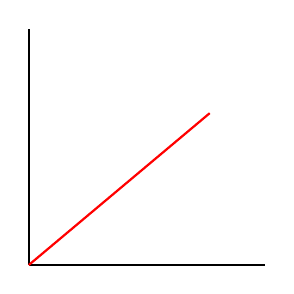
\begin{tikzpicture}
\draw [thick] ( 0,0) -- (3,0);
\draw [thick] ( 0,0) -- (0,3);
\draw [red,thick] ( 0,0) -- (400:3);
\bigangle[blue,dashed]{400}
\end{tikzpicture}
\end{document}
\end{verbatim}

% \includegraphics{https://i.stack.imgur.com/4RO8Y.png}{图片图片}


\faq{如何画交换图?}{}


\faq{如何在插入的图(\cs{includegraphics}\Arg{...})的特定位置插入符号或图}{}

可以使用 overpic 宏包,在 overpic 环境内进行图形绘制,环境内可以使用
latex 自生 picture 环境的绘图语句进行绘制。以下面给出一个例子:

\begin{verbatim}
\documentclass{article}
\usepackage{graphicx}
\usepackage{overpic}
\begin{document}
\begin{overpic}[width=0.8\textwidth
               %,grid,tics=10 % 取消注释可以产生网格线帮助定位,完成后再将其注释。
               ]{1.png}
  \put(35,10){\LaTeX}
  \put(80,0){\includegraphics[width=0.16\textwidth]{1.png}}
\end{overpic}
\end{document}
\end{verbatim}

下面左边是原图,右边是代码处理后的图片:
% \includegraphics{https://images-cdn.shimo.im/VFe2jSxjmoMZpr2B/1.png!thumbnail}
% \includegraphics{https://images-cdn.shimo.im/4qswwF2P4u44JNYB/2.png!thumbnail}

当然还有一种方法可以使用 tikz 宏包,在 tikzpicture
环境引入图片,并在此基础上进行绘图,这样的优点是绘图语句更为丰富,功能更强大。下面举个例子:

\begin{verbatim}
       ![图片](https://images-cdn.shimo.im/LrJDsfrVZIAerfPW/image.png!thumbnail)  ![图片](https://images-cdn.shimo.im/sVlNCmljor0SctYs/image.png!thumbnail)
\end{verbatim}

第一个为原图,第二个是在原图基础上添加一个标号和边.
其中的格线是用来辅助做图的。

\begin{verbatim}
\documentclass{article}
\usepackage{tikz}
\begin{document}
\pgfdeclarelayer{foreground}
\pgfdeclarelayer{background}
\pgfsetlayers{background,main,foreground}
\begin{tikzpicture}
\begin{pgfonlayer}{background}
\path[xshift=-1.24pt,yshift=4pt]      (0,0) node (o) {
  \includegraphics[width=2.8cm]{graph.pdf}};
\end{pgfonlayer}
\begin{pgfonlayer}{foreground}
    \node at (0,0) [label={[label distance=-2mm]40:$u$}]{};
    \draw[step=.5cm,help lines] (-1.4,-1.4) grid (1.4,1.4);
    \coordinate (A) at (0,1.36);
    \coordinate (B) at (0.91,-1.14);
    \fill[color=red] (B) circle (1pt);
    \draw[line width=0.6pt](A)--(B);
\end{pgfonlayer}
\end{tikzpicture}
\end{document}
\end{verbatim}

% Copyright (C) 2018 by latexstudio <http://www.latexstudio.net>
%
% This program is free software: you can redistribute it and/or modify
% it under the terms of the GNU General Public License as published by
% the Free Software Foundation, either version 3 of the License, or
% (at your option) any later version.
%
% This program is distributed in the hope that it will be useful,
% but WITHOUT ANY WARRANTY; without even the implied warranty of
% MERCHANTABILITY or FITNESS FOR A PARTICULAR PURPOSE.  See the
% GNU General Public License for more details.
%
% You should have received a copy of the GNU General Public License
% along with this program.  If not, see <http://www.gnu.org/licenses/>.
%

% !TEX root = ../latex-faq-cn.tex
% !TEX program = xelatex
% !TEX options = --shell-escape

\section{开发篇-含LaTeX3}

介绍宏开发技巧,宏包和模板类开发的常见问题。


\faq{在阅读已有的宏包或者文类时,遇到未知的命令应如何处理}{}

可以参照胡伟的《LaTeX2e文类和宏包学习手册》中的第四章-命令集注。


\faq{文档类中键值对的实现}{}

使用 xkeyval 宏包。
该宏包主要定义了以下四个命令
\begin{itemize}
  \item Ordinary keys

    最基础的键值对定义方式。说明文档中,这部分主要介绍的是 xkeyval 定义出来的宏的参数和命令。

  \item Command keys

    用于定义存放数据的宏,如美赛模板中运用了该命令来存放参赛队伍编号。

  \item Choice keys

    用于定义一个具有选择性的宏,例如以下宏
\begin{texcode}
  \define@choicekey{HTNotes.cls}{cvcolor}%
  [\val\ar]{green,orange,violet,blue}[blue]{
    \ifcase\ar\relax
      \definecolor{themecolor}{HTML}{92D14F}
      \definecolor{cvtext}{HTML}{92909B}
    \or
      \definecolor{themecolor}{RGB}{230,140,20}
      \definecolor{cvtext}{RGB}{100,100,100}
    \or
      \definecolor{themecolor}{RGB}{178,10,142}
      \definecolor{cvtext}{RGB}{100,100,100}
    \else
      \definecolor{themecolor}{RGB}{0,164,215}
      \definecolor{cvtext}{RGB}{100,100,100}
    \fi
  }
\end{texcode}
  该宏实现的是cvcolor的选择性,可以选择 green, orange, violet, blue 等参数,且 blue 为默认参数。

  \item Boolean keys

    用于定义布尔宏,用于设置开关代码。美赛模板中大部分使用的是该宏。
\end{itemize}

  具体用法请参考其说明文档。

  使用了 xkeyval 后,如何进行参数传递之类的呢?
\begin{texcode}
  \DeclareOptionX*{\PassOptionsToClass{\CurrentOption}{book}}
  \ProcessOptionsX\relax
  \LoadClass[twoside,11pt]{book}
\end{texcode}

  那么,如何定义默认参数呢?
\begin{texcode}
  \ExecuteOptionsX{
    cvcolor = {blue},
    ...
  }
\end{texcode}

  如何设置接口呢?
\begin{texcode}
  \newcommand{\HTset}[1]{\setkeys{HTNotes.cls}{#1}}
\end{texcode}

  如何检测宏是否有内容呢?并依次为基础设置开关命令?
\begin{texcode}
  % 宏定义为
  % \define@cmdkey{HTNotes.cls}[Book@]{Writer}
  \ifdefempty{\Book@Writer}{\@author}{\Book@Writer}
\end{texcode}
  该命令实现的是检测 \verb|\Book@Writer| 宏是否有内容,如果有则使用其存储的内容,无则使用 \verb|\@author| 存储的参数。

  用 xkeyval 提供的键值对实现方式,基本不会出现宏包冲突的问题,因为其前缀是由其特定的包含方式的,前提是选取适当。

% Copyright (C) 2018 by latexstudio <http://www.latexstudio.net>
%
% This program is free software: you can redistribute it and/or modify
% it under the terms of the GNU General Public License as published by
% the Free Software Foundation, either version 3 of the License, or
% (at your option) any later version.
%
% This program is distributed in the hope that it will be useful,
% but WITHOUT ANY WARRANTY; without even the implied warranty of
% MERCHANTABILITY or FITNESS FOR A PARTICULAR PURPOSE.  See the
% GNU General Public License for more details.
%
% You should have received a copy of the GNU General Public License
% along with this program.  If not, see <http://www.gnu.org/licenses/>.
%

\section{常见错误提示}

\begin{itemize}
  \item
    ! LaTeX Error: File `xxx.sty' not found.
    \cs{usepackage}时,引用错误宏包名称或者本机未下载相应的宏包。解决方法为检查拼写,或TeXLive使用tlmgr安装宏包。
  \item
    ! LaTeX Error: File `xxx.cls' not found.
    \cs{documentclass}时,引用错误文类名称或者本机未下载相应的文类。解决方法为检查拼写,或TeXLive使用tlmgr安装文类。
  \item
    ! Undefined control sequence.
    编译遇到不存在的命令(未定义的控制序列)。解决方法为检查拼写,引用相应的宏包,或者定义该命令。
  \item
    ! Missing \{ inserted. 或者 ! Missing \} inserted.
    缺少分组的某个花括号。解决方法为仔细查找上下文对应的花括号。
  \item
    ! Missing \$ inserted.
    缺少数学环境,通常为把数学环境专用的命令用在普通文本模式。
  \item
    ! LaTeX Error: Can be used only in preamble.
    有许多命令只能用于导言区,如果在document
    环境中用了这些命令,将显示上面的错误信息。
  \item
    ! LaTeX Error: Counter too large.
    计数器数值太大,一般是在需要以字母形式显示的计数器其数值超过了26。
  \item
    ! LaTeX Error: \cs{include} cannot be nested.
    在一个已经要用 \cs{include} 引入的文件中又使用了
    \cs{include} 命令。
  \item
    ! LaTeX Error: Missing |\begin{document}|
    这种情况可能是忘了输入 |\begin{document}|,或者是在导言区中有可打印的文本,还有可能是编译中断时在
    aux 等辅助文件中写入错误,对于后者,可以清理辅助文件后重新进行编译。
  \item
    ! LaTeX Error: No counter `xxx' defined.
    调用某计数器,但该计数器并不存在。
  \item
    ! LaTeX Error: No \cs{title} given. 在给出
    \cs{title} 声明之前就使用了 \cs{maketitle} 命令。
  \item
    ! LaTeX Error: Something's wrong--perhaps a missing \cs{item}.
    导致这个问题一般是在列表环境中的文本不是由 \cs{item} 开始的。
  \item
    ! LaTeX Error: There's no line here to end.
    在 \cs{par} 或空行后调用命令 \cs{newline} 或 |\\|。
    这里它们没有任何意义,如果需要额外竖直间距,应使用 \cs{vspace} 命令。
  \item
    ! LaTeX Error: Lonely \cs{item} -- perhaps a missing list enviroment.
    在列表环境外使用了 \cs{item} 命令。
\end{itemize}

% Copyright (C) 2018 by latexstudio <http://www.latexstudio.net>
%
% This program is free software: you can redistribute it and/or modify
% it under the terms of the GNU General Public License as published by
% the Free Software Foundation, either version 3 of the License, or
% (at your option) any later version.
%
% This program is distributed in the hope that it will be useful,
% but WITHOUT ANY WARRANTY; without even the implied warranty of
% MERCHANTABILITY or FITNESS FOR A PARTICULAR PURPOSE.  See the
% GNU General Public License for more details.
%
% You should have received a copy of the GNU General Public License
% along with this program.  If not, see <http://www.gnu.org/licenses/>.
%

\section{用法惯例}


\faq{TeX编辑器中的魔法注释}{}

在TeX中有单行注释命令为\%,其后的文本主要是对源代码进行一些说明,它们会被TeX,LaTeX等排版引擎所忽略。但有些
注释对专门的TeX相关编辑器来说,可能用特别的意义。在不同的TeX编辑器中,这魔法注释(magic comments)可能是不同
的。 下面是一些例子:
\begin{itemize}
  \item 指定\TeX{}编译器
  \begin{verbatim}
  TeXStudio,TeXworks, Sublime Text
  % !TeX program = xelatex
  
  TeXShop
  %!TEX TS-program = xelatex
  \end{verbatim}
  同理,将 xelatex 变为 pdflatex,就可以强制调用 pdfLaTeX 编译器。
  在代码中需要使用ifxetex宏包进行条件判断。 
  \item 指定文档为 |UTF-8| 编码
  \begin{verbatim}
  TeXworks,TeXStudio, Sublime Text
  % !TeX encoding = utf8
  
  Winedt
  % !Mode:: "TeX:UTF-8"
  or
  % -*- coding: utf-8 -*-
  
  TeXShop
  %!TEX encoding = UTF-8 Unicode
  \end{verbatim}
  由于Winedt对编码自动识别能力较弱,使用此注释比较必要,不然要手动设置。
  \item 指定主文档
  \begin{verbatim}
  TeXStudio, Sublime Text
  % !TeX root = filename
  \end{verbatim}
  若需要指定上一层次的文件,则应该使用以下命令
  \begin{verbatim}
  TeXStudio, Sublime Text
  % !TeX root = ../main.tex
  \end{verbatim}
  用两点表示返回上一层次,如果还需要再返回一个层次,则需要
  \begin{verbatim}
  TeXStudio, Sublime Text
  % !TeX root = ../../main.tex
  \end{verbatim}
  \item 指定bib处理程序
  \begin{verbatim}
  TeXStudio
  % !TeX TXS-program:bibliography = txs:///biber
  \end{verbatim}
  源文件添加如上代码即可用biber处理bib文件。将biber改为bibtex,即可指定\BibTeX{}处理bib文件。
  \item 
  为\TeX{}编译器指定参数
  \begin{verbatim}
  TeXStudio
  % !TeX TXS-program:compile = txs:///xelatex/[--shell-escape]
  
  sublime text - latextools
  %!TEX options = --shell-escape
  
  texshop
  -shell-escape
  \end{verbatim}
  有时在使用某些宏包时我们需要额外调用一些编译参数,例如 minted 宏包需要使用 --shell-escape,这时可用以上魔法注释实现该功能
\end{itemize}

各种编辑器对魔法注释的支持情况见表~\ref{magiccommands}
\begin{table}
  \centering
  \caption{各种编辑器对魔法注释的支持情况。x表示支持;o表示不支持;?表示不确定}\label{magiccommands}
  \begin{tabular}{|l|*{4}{c|}}
    \hline
    & Encoding & Program & Root & Spellcheck \\
    \hline
    TeXShop & x  & x & x & x \\
    \hline
    TeXStudio & x & x & x & x \\
    \hline
    TextMate & ? & x & x & ? \\
    \hline
    TeXworks & x & x & x & x \\
    \hline
    SublimeText  & x & x & x & x \\ 
    \hline
    VSCode & x & x & ? & ? \\
    \hline
    Atom & o & x & x & o \\
    \hline
    Vim
    (vimtex) & o & x & x & o \\ 
    \hline
    Texpad & o & o & ? & ? \\
    \hline
  \end{tabular}
\end{table}

\section{其它}

\faq{LaTeX与数学软件(Mathematica, Maple,Sagemath等)}{}


\faq{LaTeX与公式编辑器}{}

公式编辑器MathType设置下就可以输入TeX指令得到公式,也可以复制公式得到TeX指令,但是得到的指令是所谓的机器代
码,可读性实在不敢恭维。

\faq{MathJax}{}
MathJax是一个JavaScript引擎,用来显示网络上的数学公式。它支持LaTeX、MathML、AsciiMath符号。查阅MathJax支
持的LaTeX命令请参考\url{http://onemathematicalcat.org/MathJaxDocumentation/TeXSyntax.htm}

\end{document}
